\documentclass[11pt]{article}
\usepackage[T1]{fontenc}
\usepackage[utf8]{inputenc}
\usepackage{lmodern}
\usepackage[margin=1in]{geometry}
\usepackage{amsmath,amssymb,mathtools,amsthm}
\usepackage{microtype,enumitem,booktabs,array}
\usepackage{flafter,placeins}
\usepackage{tikz}
\usetikzlibrary{arrows.meta,positioning,fit,backgrounds,calc,patterns,decorations.pathreplacing}
\usepackage{xcolor}
\definecolor{linkblue}{RGB}{28,62,101}
\definecolor{figureblue}{RGB}{223,234,246}
\definecolor{figuregray}{RGB}{242,244,247}
\usepackage[colorlinks=true,linkcolor=linkblue,citecolor=linkblue,urlcolor=linkblue,bookmarksnumbered=true,bookmarksdepth=2,pdfusetitle]{hyperref}
\setcounter{tocdepth}{2}
\urlstyle{same}
\usepackage[nameinlink,capitalise,noabbrev]{cleveref}
\numberwithin{equation}{section}
\newtheorem{theorem}{Theorem}[section]
\newtheorem{proposition}[theorem]{Proposition}
\newtheorem{lemma}[theorem]{Lemma}
\newtheorem{corollary}[theorem]{Corollary}
\theoremstyle{definition}
\newtheorem{definition}[theorem]{Definition}
\newtheorem{notation}[theorem]{Notation}
\theoremstyle{remark}
\newtheorem{remark}[theorem]{Remark}
\newtheorem{example}[theorem]{Example}
\DeclareMathOperator{\Env}{Env}
\DeclareMathOperator{\rank}{rank}
\DeclareMathOperator{\mult}{mult}
\DeclareMathOperator{\Span}{span}
\DeclareMathOperator{\codim}{codim}
\DeclareMathOperator{\Spec}{Spec}
\DeclareMathOperator{\Sing}{Sing}
\DeclareMathOperator{\supp}{supp}
\DeclareMathOperator{\tr}{tr}
\DeclareMathOperator{\Res}{Res}
\DeclareMathOperator{\lcm}{lcm}
\newcommand{\R}{\mathbb R}
\newcommand{\C}{\mathbb C}
\newcommand{\PP}{\mathbb P}
\newcommand{\E}{\mathbb E}
\newcommand{\Prob}{\mathbb P}
\setlength{\emergencystretch}{1.5em}
\allowdisplaybreaks[2]
\raggedbottom
\clubpenalty=10000
\widowpenalty=10000
\usepackage{needspace,etoolbox}
\pretocmd{\subsection}{\Needspace{9\baselineskip}}{}{\PackageError{paper}{Subsection spacing hook failed}{}}
\BeforeBeginEnvironment{theorem}{\Needspace{5\baselineskip}}
\BeforeBeginEnvironment{proposition}{\Needspace{5\baselineskip}}
\BeforeBeginEnvironment{lemma}{\Needspace{5\baselineskip}}
\BeforeBeginEnvironment{corollary}{\Needspace{5\baselineskip}}
\BeforeBeginEnvironment{remark}{\Needspace{5\baselineskip}}

\title{The higher-dimensional Erd\H{o}s distinct-distances conjecture}
\author{OpenAI}
\date{September 23, 2026}
\begin{document}
\maketitle
\begin{abstract}
For every fixed integer $d\ge3$, we prove that every set of $n\ge2$ distinct
points in $\mathbb R^d$ determines at least $c_d n^{2/d}$ distinct
distances, where $c_d>0$ depends only on $d$. This resolves the
higher-dimensional Erd\H{o}s distinct-distances conjecture positively.
\end{abstract}
\section{Introduction}\label{sec:introduction}

For a finite set \(P\subset\mathbb R^d\), write
\[
 \Delta(P)=\{|p-q|:p,q\in P,\ p\ne q\}.
\]
The distinct-distances problem asks how small \(|\Delta(P)|\) can be
among all sets of a prescribed cardinality. Erd\H{o}s introduced the
problem in 1946~\cite{erdos1946}. It relates a simple metric statistic
to the geometric structure of a finite set: when distances are few,
many pairs repeat their lengths, but the arrangement of those repetitions is
constrained by Euclidean geometry.
The higher-dimensional conjecture predicts a constant multiple of
\(n^{2/d}\) distances among any \(n\) points of \(\mathbb R^d\), for
every fixed \(d\ge3\); see, for example,
\cite{BardwellEvansSheffer2019,tidoryuzakharov2026}.
We prove this prediction.

\begin{theorem}\label{thm:main}
For every integer \(d\ge3\), there is a constant \(c_d>0\) such that
every finite set \(P\subset\mathbb R^d\) of \(n\ge2\) distinct points
satisfies
\[
 |\Delta(P)|\ge c_d n^{2/d}.
\]
\end{theorem}

This resolves the higher-dimensional Erd\H{o}s distinct-distances
conjecture positively. No assumption is made on the position, spacing,
or concentration of the points. The power of \(n\) is optimal:
the integer grid \(\{1,\ldots,t\}^d\) has \(t^d\) points, and its squared
distances are integers between \(1\) and \(d(t-1)^2\). In the plane,
the square-grid construction gives \(O(n/\sqrt{\log n})\)
distances~\cite{erdos1946}; the planar problem consequently
has a different conjectural order.

\subsection{Historical context and the methods of the proof}

Higher-dimensional distance estimates developed in part through
incidence bounds for curves and spheres. Clarkson, Edelsbrunner,
Guibas, Sharir, and Welzl bounded the number of pairs realizing a fixed
positive distance in three dimensions, giving a distinct-distance
lower bound at the square-root scale, up to a slowly growing
factor~\cite{ClarksonEdelsbrunnerGuibasSharirWelzl1990}.
Aronov, Pach, Sharir, and Tardos improved the three-dimensional lower
bound to \(\Omega_\varepsilon(n^{77/141-\varepsilon})\) for each
\(\varepsilon>0\) and propagated improvements to higher
dimensions~\cite{AronovPachSharirTardos2004}.
Their three-dimensional estimate is \emph{pinned}: it finds a point
of the given set from which that many distinct distances occur.

Solymosi and Vu developed two recursive inequalities connecting
distance bounds in lower and higher dimensions
\cite[Theorems~2.1--2.2]{SolymosiVu2008}.
The recurrences have separate forms for the total number of distances
and for the maximum number measured from one point of the set. We use
the forms for total distances in the comparisons below. Their original theorem gives
\(\Omega(n^{0.5643})\) distances in dimension three and
\(\Omega_d(n^{2/d-2/(d(d+2))})\) for every fixed \(d\ge4\)
\cite[Theorem~1.1]{SolymosiVu2008}.

A different approach counts repeated distances through rigid motions
matching subsets of the point sets. Elekes and Sharir developed this viewpoint for the planar
problem~\cite{elekessharir2011}. Guth and Katz reduced the resulting
planar motion count to incidences of points and lines in three-dimensional
space and combined polynomial partitioning with ruled-surface geometry to prove
the planar bound \(\Omega(n/\log n)\)
\cite[Theorem~1.1 and Sections~2--4]{guthkatz2015}.
That bound supplies the two-dimensional input to our induction.
Bardwell-Evans and Sheffer extended the rigid-motion approach to
higher dimensions through a reduction to incidences of
\((d-1)\)-flats in \(\mathbb R^{2d-1}\)
\cite{BardwellEvansSheffer2019}. Their work identifies structural
restrictions on the resulting flats and the need to control their
concentration in algebraic varieties.

Combining the Guth--Katz planar bound with the first Solymosi--Vu
recurrence gives \(\Omega(n^{3/5}/(\log n)^{2/5})\) distances in
dimension three~\cite[Theorem~2.1]{SolymosiVu2008}.
More recently, Tidor, Yu, and Zakharov proved
\(n^{2/3-o(1)}\) distinct distances for arbitrary point sets in
\(\mathbb R^3\)~\cite[Theorem~1.1]{tidoryuzakharov2026}.
Inserting their three-dimensional distance bound into the Solymosi--Vu
recurrences gives \(n^{8/17-o(1)}\) in dimension four and
\(n^{3/8-o(1)}\) in dimension five
\cite[Corollaries~2.3 and~2.6]{SolymosiVu2008}.
The \(o(1)\) terms here absorb the subpolynomial loss in that input.
The leading exponents in these two deductions still fall below the
conjectured value \(2/d\).
Bounds for points on prescribed surfaces, or for distances from a
single point, have different hypotheses or conclusions.\footnote{An
earlier manuscript of Aksoy Yazici claimed
the constant-factor bound in all dimensions \(d\ge3\), but was
withdrawn by the author because the proof of its Theorem~1.2 is not
correct~\cite{AksoyYazici2020Withdrawn}.}

Tidor, Yu, and Zakharov's proof develops rigid-motion flat geometry,
regular approximate complete intersections, and degree-sensitive
incidence estimates. These methods provide close antecedents for
several parts of the argument below: the physical and
opposite-orientation flat families, the recovery of actual families
of contained flats from tangent data, and the geometric treatment of
projected curves
\cite[Sections~3--6 and~10.2--10.3]{tidoryuzakharov2026}.

The algebraic argument draws on Hilbert function estimates of Chardin
and Chardin--Philippon
\cite{chardin1989,chardinphilippon1999,chardinphilippon2002erratum},
and on Walsh's work on approximate complete intersections and
algebraic concentration~\cite{walsh2020,walsh2023}.
Hilbert functions measure how many independent
polynomial conditions a set can impose. Approximate complete
intersections cut out an irreducible variety as a component of the
common zero set of equations whose product of degrees is controlled
by the variety's degree.
We use these two ideas to keep track of concentration at several
polynomial degree scales. The uniform concentration theorem for
evaluation flats of skew forms, including its exceptional parameter
families, is proved in full in Appendix~\ref{conc:section}.
The real incidence arguments, including the planar distinct-distance
bound, are supplied in Appendix~\ref{ci:section}; their relation to
the work of Szemer\'edi--Trotter, Beck, Elekes--Sharir, and Guth--Katz
is recorded where each argument is used.

\subsection{Why the constant factor matters}

An estimate \(|\Delta(P)|\ge n^{2/d-o(1)}\) does not by itself imply
Theorem~\ref{thm:main}. The ratio \(|\Delta(P)|/n^{2/d}\) could still
tend to zero more slowly than every negative power of \(n\).
To obtain a constant factor, the proof must exclude every such
sequence, without first fixing a power saving.

We therefore argue in the least dimension \(d\ge3\) in which the
theorem could fail, and use the notation
\[
 N=|P|,\qquad B=N^{1/d},\qquad A=B^2,\qquad
 M=1+|\Delta(P)|.
\]
Failure would give a sequence with \(N\to\infty\) and \(M/A\to0\).
The lower-dimensional bounds limit the number of points in any
proper affine flat. They do not prevent substantial concentration
on more general varieties, nor do they identify a single polynomial
degree at which all of that concentration can be studied.
The multiscale argument below addresses this second difficulty.

\subsection{Overview of the proof}

\paragraph{1. Select directions that admit interpolation.}
For distinct points \(p,q\), let
\(\pi_p(q)=[q-p]\in\mathbb P^{d-1}\) denote their projective direction.
We seek a positive fraction of the unordered pairs of points such
that, at each center \(p\), homogeneous polynomials of degree
\(\lfloor A\rfloor\) can prescribe arbitrary values at the selected
displacement vectors \(q-p\). Equivalently, the corresponding evaluation
vectors are linearly independent. The selection must be symmetric:
a pair is retained or removed at both endpoints.

The principal geometric obstruction would be a collection \(C_p\)
of projective curves at each center, each curve spanning at most a
projective plane, with total degree \(o(N/A)\), such that almost
every pair \(\{p,q\}\) satisfies
\[
 \pi_p(q)\in C_p\quad\hbox{or}\quad\pi_q(p)\in C_q.
\]
The union of the corresponding lines through \(p\) is a cone;
the small total degree explains the term \emph{sparse cones}.
Theorem~\ref{sc:theorem} rules out this coverage, including the
choice of either endpoint for each pair. Once it is excluded, greedy
removal of curves containing too many directions leaves a positive
fraction of pairs with controlled concentration on every projective
variety. A maximal symmetric selection then gives the interpolation
property (Propositions~\ref{red:directions} and
\ref{red:independent-stars}). This last linear-algebra argument costs
only a fixed fraction of pairs.

\paragraph{2. Exclude sparse cones at all degree scales.}
The sparse-cones theorem occupies the central part of the paper.
Section~\ref{sec:profiles} divides the point set according to how
successive polynomial equations cut down the dimension of the
varieties containing its points. It tests degrees in windows
\([B e^{-s},B e^s]\) with several width parameters \(s\), instead of
fixing a single power of \(N\). Points isolated by equations of
sufficiently small degree form a core that is handled directly.
Each remaining piece carries a fixed chain of proper hypersurface
cuts, ending in isolated points.
A cut is proper when its equation does not vanish identically on
the component being cut. The testing degrees at these cuts form a
\emph{scale profile}. Between consecutive cuts, the dimension stays
constant, and Hilbert-function estimates give a lower bound on the
growth of polynomial restriction rank. B\'ezout's theorem bounds
the degrees and point counts of the intervening components.

The comparison uses labels \((p,\pi_p(q))\), which record both the
center and the direction of an ordered pair. At each fixed center,
sparse-cone coverage puts the directions on curves of small total
degree, limiting their polynomial rank. The profiles give an incompatible rank lower bound
for a positive fraction of pairs. A complication is that radial
projection can identify several components, or several points on
one component. Section~\ref{geo:section} controls this behavior by
secant geometry. For separated windows, Subsection~\ref{dep:section}
bounds the resulting loss of degree at the actual centers.

Two limiting cases leave no strict margin in the general rank
comparison. At the outermost degree window, common equations with
independent differentials on most components allow a direct geometric
comparison of their projected images. At the last one-dimensional
stage for narrower center windows, the argument identifies the projection
of the assigned terminal curve with a curve in the covering family.
A global estimate has already removed all such incidences at a
cost of \(o(N^2)\) pairs (Proposition~\ref{geo:terminal}). These two
arguments in Section~\ref{sec:sparse-cones} supply the endpoint
control needed for an arbitrarily slow limit \(M/A\to0\).

\paragraph{3. Turn equal distances into intersections of flats.}
Take a generic rotated copy \(Q\) of \(P\) and transport the selected
pairs to \(Q\). For \((p,q)\in P\times Q\),
consider the affine flat
\[
 F_{p,q}=\{(Z,c):Z(p+q)/2+c=(p-q)/2\},
 \qquad Z^{\mathsf T}=-Z,\quad c\in\mathbb C^d.
\]
The coordinates \((Z,c)\) identify with skew forms on
\(\mathbb C^{d+1}\) by adjoining \(c\) as the last column and
\(-c^{\mathsf T}\) as the last row, with last diagonal entry zero.
Join \((p,q)\) to \((p',q')\)
when both physical pairs have been selected in Step 1 and
\(|p-p'|=|q-q'|\). Cauchy--Schwarz gives
\(\Omega(N^4/M)\) edges. On \(F_{p,q}\), the intersection with a
neighbor is the flat defined by
\[
 Z(u+w)=u-w,\qquad u=p'-p,\quad w=q'-q.
\]
The interpolation property ensures that these local flats are
distinct and that their parameters have polynomial separators of
degree \(O(A)\): one parameter can be distinguished from all the
others by a polynomial of that degree.

Appendix~\ref{conc:section} proves concentration bounds for these
evaluation flats, both in the full skew-form space and inside one
fixed pair flat. In the local application an exceptional parameter
family corresponds to many matches under one rigid motion. For
\(d\ge4\), its required size bound follows from the total number of
points. For \(d=3\), Section~\ref{mot:section} bounds
\(\sum_g |gP\cap Q|^2\) over motions with at least \(CA\) matches
by \(O(N^4/A)\), with both orientations included. Removing the
corresponding edges costs \(o(N^4/M)\). After this removal and
pruning vertices of small degree, the minimum number of neighbors,
divided by \(A^{d-1}\), tends to infinity.
The local concentration bound says that
a nonzero polynomial of degree at most \(A\) on a pair flat can
vanish on at most \(O(A^{d-1})\) of its neighbor flats.

\paragraph{4. Sample once and compare polynomial ranks.}
The remaining contradiction is short. Sample the retained pair flats
independently with a small fixed probability. With positive probability,
the sample is small enough that the global concentration bound forces
the whole family to impose more independent polynomial conditions
in degree \(\lfloor A\rfloor\) than the sample. Simultaneously,
every retained flat has more than \(CA^{d-1}\) sampled neighbors.
Thus a polynomial of degree at most \(\lfloor A\rfloor\) vanishes on every sampled flat
but is nonzero on at least one retained flat \(F\).
The restriction of the polynomial to
\(F\) then violates local concentration. The sample uses one fixed
probability, and all concentration constants are uniform; this is
where the preceding quantitative estimates produce the positive
constant in Theorem~\ref{thm:main}.

\paragraph{Organization and prerequisites.}
Section~\ref{sec:reduction} carries out Steps 1, 3, and 4, assuming
the sparse-cones, concentration, and rich-motion theorems. It can
therefore be read first as the formal assembly of the argument.
Section~\ref{poly:section} proves the polynomial interpolation,
regularity, and multiplicity estimates. Sections~\ref{geo:section}
through~\ref{sec:sparse-cones} establish the geometric and multiscale
arguments of Step 2. Section~\ref{mot:section} proves the rich-motion
estimate, and Appendices~\ref{conc:section} and~\ref{ci:section}
provide the concentration and real incidence foundations.
Figure~\ref{fig:proof-map} summarizes the principal dependencies.
We use characteristic-zero algebraic geometry, including projective
degree and B\'ezout's theorem, generic linear sections, regular local
rings and Koszul resolutions, and projective-bundle intersection
formulas. The precise forms needed are specified where they are
used. Constants may depend on the fixed ambient dimension; any
additional dependence is indicated explicitly.

\begin{figure}[htbp]
\centering
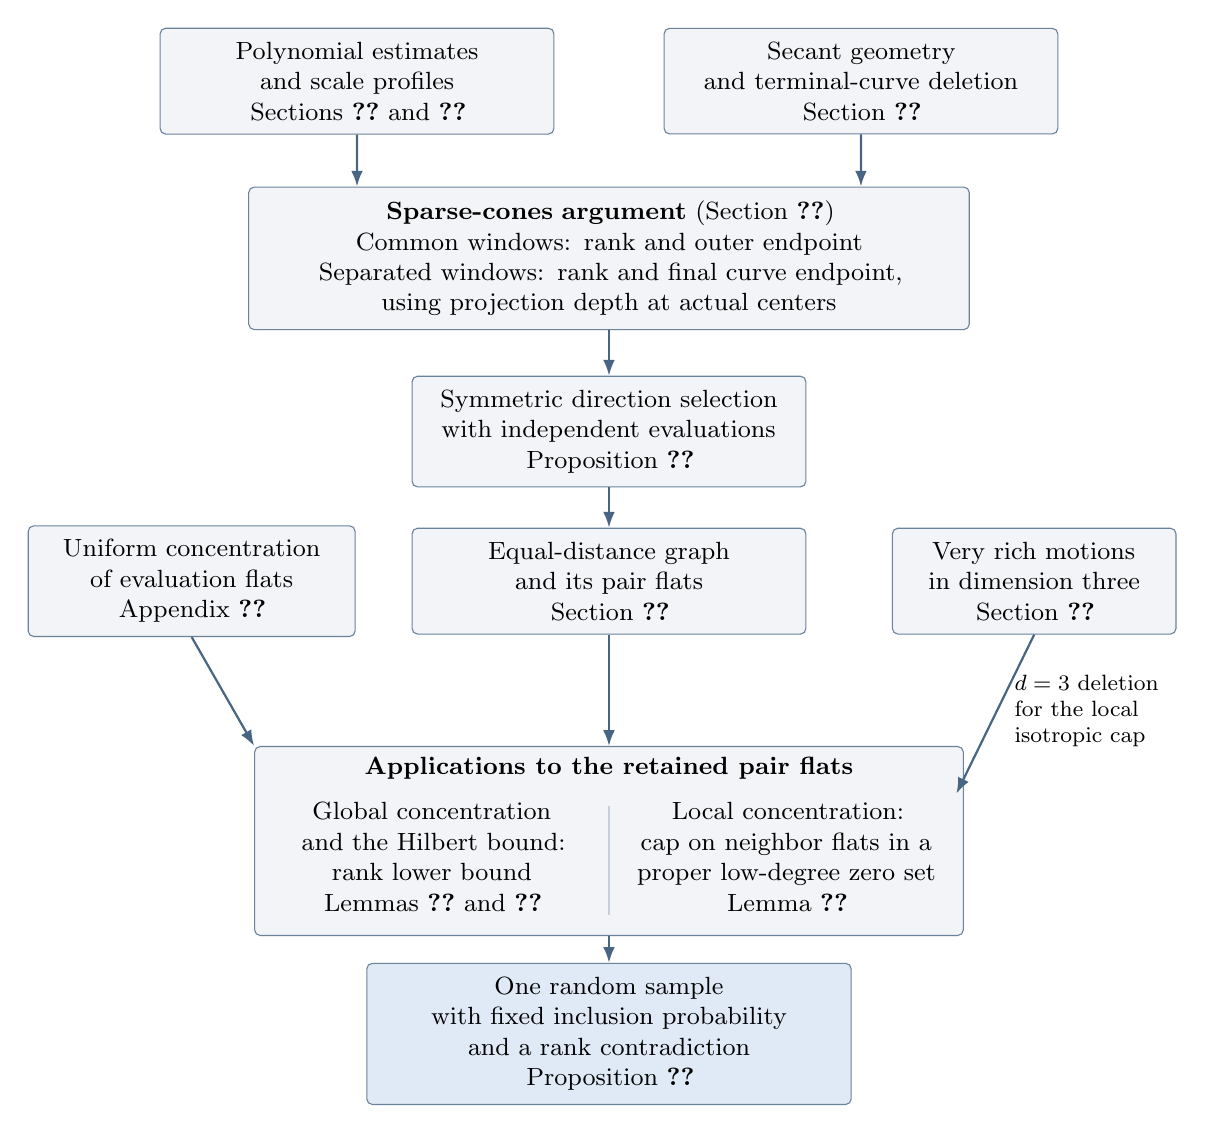
\begin{tikzpicture}[
 box/.style={draw=linkblue!65,rounded corners=2pt,fill=figuregray,
             align=center,font=\small,text width=4.65cm,
             minimum height=1.15cm,inner sep=5pt},
 application/.style={align=center,font=\small,text width=4.1cm,
                     inner sep=3pt},
 arrow/.style={-{Latex[length=2mm]},thick,draw=linkblue!80}]
 \node[box] (poly) at (-3.2,0.65)
   {Polynomial estimates\\and scale profiles\\
    Sections~\ref{poly:section} and~\ref{sec:profiles}};
 \node[box] (geo) at (3.2,0.65)
   {Secant geometry\\and terminal-curve deletion\\
    Section~\ref{geo:section}};
 \node[box,text width=8.8cm] (sparse) at (0,-1.6)
   {\textbf{Sparse-cones argument} (Section~\ref{sec:sparse-cones})\\
    Common windows: rank and outer endpoint\\
    Separated windows: rank and final curve endpoint,\\
    using projection depth at actual centers};
 \node[box] (stars) at (0,-3.8)
   {Symmetric direction selection\\with independent evaluations\\
    Proposition~\ref{red:independent-stars}};
 \node[box] (graph) at (0,-5.7)
   {Equal-distance graph\\and its pair flats\\
    Section~\ref{sec:reduction}};
 \node[box,text width=3.8cm] (conc) at (-5.3,-5.7)
   {Uniform concentration\\of evaluation flats\\
    Appendix~\ref{conc:section}};
 \node[box,text width=3.25cm] (motions) at (5.4,-5.7)
   {Very rich motions\\in dimension three\\
    Section~\ref{mot:section}};

 \node[draw=linkblue!65,rounded corners=2pt,fill=figuregray,
       minimum width=9cm,minimum height=2.4cm,inner sep=0pt]
       (applications) at (0,-9) {};
 \node[font=\small\bfseries,align=center] at (0,-8.08)
   {Applications to the retained pair flats};
 \node[application] (global) at (-2.25,-9.2)
   {Global concentration\\and the Hilbert bound:\\rank lower bound\\
    Lemmas~\ref{red:global-concentration} and~\ref{poly:hilbert}};
 \node[application] (local) at (2.25,-9.2)
   {Local concentration:\\cap on neighbor flats in a\\
    proper low-degree zero set\\
    Lemma~\ref{red:local-concentration}};
 \draw[linkblue!25] (0,-8.55) -- (0,-9.94);

 \node[box,text width=5.8cm,fill=figureblue] (end) at (0,-11.45)
   {One random sample\\with fixed inclusion probability\\
    and a rank contradiction\\
    Proposition~\ref{red:main-contradiction}};

 \draw[arrow] (poly.south) -- ([xshift=-3.2cm]sparse.north);
 \draw[arrow] (geo.south) -- ([xshift=3.2cm]sparse.north);
 \draw[arrow] (sparse.south) -- (stars.north);
 \draw[arrow] (stars.south) -- (graph.north);
 \draw[arrow] (graph.south) -- (applications.north);
 \draw[arrow] (conc.south) -- (applications.north west);
 \draw[arrow] (motions.south) --
   node[pos=.48,right,xshift=3pt,align=left,font=\footnotesize,inner sep=3pt]
        {\(d=3\) deletion\\for the local\\isotropic cap}
   (local.north east);
 \draw[arrow] (applications.south) -- (end.north);
\end{tikzpicture}

\caption{Principal dependencies. Both endpoint arguments belong to the
sparse-cones theorem. The separated-window argument uses projection depth
at actual centers. Global concentration combines with the component
Hilbert bound; the rich-motion bound permits the \(d=3\) edge deletion
that supplies the local isotropic cap. The contradiction uses one sample with a
fixed inclusion probability. Appendix~\ref{ci:section} supplies the planar
induction base and the real incidence inputs to the geometric and motion
arguments.}
\label{fig:proof-map}
\end{figure}

\FloatBarrier
\tableofcontents
\section{The reduction to sparse cones and concentration}
\label{sec:reduction}

This section proves Theorem~\ref{thm:main} from the sparse-cones theorem,
the rich-motion theorem, and the uniform concentration theorem.
Their proofs occupy the later sections and appendices. We include the
selection and sampling arguments here, since keeping their constants
uniform is essential.

\subsection{The contradiction regime}

Suppose that Theorem~\ref{thm:main} fails, and take the least dimension
\(d\ge3\) in which it fails. There is then a sequence of finite sets
\(P\subset\mathbb R^d\) for which, with
\begin{equation}\label{red:regime}
 N=|P|,\qquad M=1+|\Delta(P)|,\qquad
 B=N^{1/d},\qquad A=B^2,
 \qquad N\longrightarrow\infty,\quad M/A\longrightarrow0.
\end{equation}
Here and below a statement along the sequence is understood after
discarding finitely many terms, if necessary. The fact that
\(N\to\infty\) follows because a set of at least two points determines
at least one distance. Adding \(1\) to the number of distances does
not affect the vanishing ratio.

For \(3\le u<d\), the assertion in dimension \(u\) is available by
minimality of \(d\). We also use the planar result proved in
Theorem~\ref{ci:planar-distances}. These give the following bounds.

\begin{lemma}[Occupancy of proper flats]\label{red:flat-caps}
In the regime~\eqref{red:regime}, a real affine \(u\)-flat contains
at most
\[
 \begin{cases}
  1,&u=0,\\
  2M,&u=1,\\
  C M\log(2M),&u=2,\\
  C_u M^{u/2},&3\le u<d
 \end{cases}
\]
points of \(P\). A circle contains at most \(2M\) points.
In particular there is a fixed \(c_0>0\) such that every proper real
affine flat contains at most \(N B^{-c_0}\) points for all sufficiently
large terms of the sequence. The same assertion holds for a proper
complex affine flat when only its real sample points are counted.
Planes have the more precise bound \(B^{2+o(1)}\).
\end{lemma}

\begin{proof}
From a point on a line, any positive distance has at most two realizations
on that line. For a circle, use a sample point on the circle: the
intersection with a circle of prescribed positive radius about that
point has at most two points. These observations include the sample
point itself after using \(M=1+|\Delta(P)|\).

The planar bound is Corollary~\ref{ci:planar-occupancy}. The other bounds
follow by applying the lower-dimensional assertion to the points in
the flat, whose pairwise distances are among the distances of \(P\).
Since \(M\le B^2\), the planar bound is \(O(B^2\log B)\), while a proper
flat of dimension \(u\ge3\) contains \(O(B^u)\) points. Thus, for example,
\(c_0=1/2\) works after advancing along the sequence. A complex affine
flat containing real points contains their real affine span, whose
real dimension is at most its complex dimension. Applying the real
bound to that span proves the last assertion.
\end{proof}

We use complex varieties for polynomial arguments. Degree means the
degree of the projective closure; for a family of components of a fixed
dimension it means the sum of their degrees. A projective direction
from \(p\) is denoted by
\[
 \pi_p(q)=[q-p]\in\mathbb P^{d-1}.
\]
Restriction of polynomials of degree at most \(D\) to an affine set
\(T\) has rank \(H_T(D)\). In projective space we use homogeneous
polynomials of degree exactly \(D\). The degree-\(D\) envelope
\(\Env_D(T)\) is the common zero locus of all such polynomials
vanishing on \(T\). Its rank at that degree equals \(H_T(D)\).

Here is the form of the sparse-cones theorem that we will use.

\begin{quote}
In the regime~\eqref{red:regime}, one cannot assign to each \(p\in P\)
a union \(C_p\) of irreducible projective curves, each spanning a
projective space of dimension at most two, with
\[
 \deg C_p\le\delta N/A,\qquad\delta\to0,
\]
such that all but \(o(N^2)\) unordered pairs \(\{p,q\}\) satisfy
\(\pi_p(q)\in C_p\) or \(\pi_q(p)\in C_q\).
\end{quote}
This is Theorem~\ref{sc:theorem}. Both the alternative between the two
endpoints and the absence of a prescribed rate for \(\delta\) are
important.

\subsection{A symmetric selection of directions}

\begin{proposition}\label{red:directions}
After passing to a subsequence, there is an undirected graph
\(\mathcal G\) on \(P\) with at least \(cN^2\) edges such that, for every
vertex \(p\) and every irreducible projective variety
\(Y\subset\mathbb P^{d-1}\) of dimension \(a\),
\begin{equation}\label{eq:direction-count}
 \#\{q:\{p,q\}\in\mathcal G,\ \pi_p(q)\in Y\}
 \le C\,\deg(Y)A^a.
\end{equation}
The positive constants \(c,C\) are fixed along the subsequence.
\end{proposition}

\begin{proof}
First discard pairs on lines containing more than \(H\) sample points,
where \(H\) will be a sufficiently large fixed constant.
A generic planar projection preserves the relevant distinct points,
lines, and incidences. The rich-line consequence of
Theorem~\ref{ci:st} therefore bounds the number of physical lines with
at least \(t\) points by
\[
 C(N^2/t^3+N/t),\qquad t\ge2.
\]
If \(L_{\max}=o(N)\) is the maximum occupancy, a dyadic sum gives
\[
 \#\{\text{discarded pairs}\}
 \le C N^2/H+C N L_{\max}=O(N^2/H)+o(N^2).
\]

At each \(p\), independently of the other stars, greedily remove
directions on any irreducible curve spanning at most a projective plane
that currently contains more than \(K A\) times its degree many
partners. Each removal contains at least one previously unremoved
partner, so the process terminates. Record the curves chosen in that
star. Their total degree is at most \(N/(KA)\), because their charged
partner sets are disjoint. Now keep an unordered pair only when it
survived both endpoint procedures.

There must be fixed \(H,K\) and a subsequence on which a positive
fraction of pairs survives. Otherwise, a diagonal choice with
\(H,K\to\infty\) sufficiently slowly would make the surviving fraction
tend to zero, while the first, rich-line discard also has vanishing
fraction. The recorded curves would then cover all but \(o(N^2)\)
pairs from one endpoint or the other and have total degree at most
\(N/(KA)=o(N/A)\) in every star. This contradicts
Theorem~\ref{sc:theorem}. Fix such \(H,K\) and a positive-density
subsequence.

We prove~\eqref{eq:direction-count} by induction on \(a\). For \(a=0\)
it is the light-line bound. Fix a variety \(Y\) of dimension \(a\ge1\),
a center \(p\), and the selected partners counted on \(Y\). Let \(U\)
be the real linear span of their displacements from \(p\), and put
\(\ell=\dim U\). There is nothing to prove if this collection is empty.

Consider a full radius class about \(p\), meaning all points of \(P\)
at one prescribed distance from \(p\). Suppose it has \(L\ge2M\)
distinct orthogonal projections to \(U\), and choose physical points
\(z_1,\ldots,z_L\in P\) in that class representing those projections.
For each counted partner \(q\), the distances
\(|q-z_i|\), including zero when it occurs, take at most \(M\) values.
Consequently at least
\[
 L^2/M-L\ge L^2/(2M)
\]
ordered pairs \(i\ne j\) have equal distance to \(q\).
As the \(z_i\) lie in a common radius class,
\[
 |q-z_i|=|q-z_j|
 \quad\Longrightarrow\quad
 (q-p)\cdot(z_i-z_j)=0.
\]
The projection of \(z_i-z_j\) to \(U\) is nonzero. The resulting
hyperplane section is proper on \(Y\): if its linear equation vanished
on \(Y\), it would vanish on all counted displacements and hence on
\(U\), which is impossible for its nonzero normal in \(U\).
B\'ezout's theorem and the induction hypothesis bound the number of
partners on each section by \(C\deg(Y)A^{a-1}\). Double counting gives
\[
 \#\{q\text{ counted}\}\frac{L^2}{2M}
 \le C L^2\deg(Y)A^{a-1}.
\]
This is~\eqref{eq:direction-count}, since \(M\le A\).

In the remaining case, each of the at most \(M\) radius classes has
fewer than \(2M\) projections to \(U\). Thus the full sample has
\(O(M^2)\) fibers on which both the radius about \(p\) and the
projection to \(U\) are fixed.
A fiber lies on a sphere in an affine space of dimension \(d-\ell\).
If \(\ell\ge4\) and \(d-\ell\ge3\), lower-dimensional induction bounds
each fiber by \(O(M^{(d-\ell)/2})\). If \(d-\ell=2\), the circle bound
is \(O(M)\); if \(d-\ell\le1\), the fiber has at most two points.
In all cases the total is \(O(M^{d/2})\), contradicting
\(N/M^{d/2}\to\infty\). Thus this alternative is impossible when
\(\ell\ge4\).

It remains to consider \(\ell\le3\).
For \(a\ge2\), Lemma~\ref{red:flat-caps} bounds the counted partners
by \(O(A^2)\), which is sufficient. If the span is the entire space,
then \(d=3\) and the trivial bound \(N=A^{3/2}\) is sufficient instead.
For \(a=1\), either \(Y\subset\mathbb P(U_{\mathbb C})\), in which case
the greedy curve bound applies, or its intersection with that
projective subspace is proper and consists of at most \(\deg Y\)
points. The light-line bound handles the latter case. This completes
the induction. Fixed increases in the constants at the finitely many
dimensions are harmless.
\end{proof}

\begin{proposition}[Independent evaluations in every star]
\label{red:independent-stars}
A further symmetric selection retains at least \(c'N^2\) pairs and
has the following property: the direction-evaluation vectors of the
partners in each star are linearly independent for homogeneous
polynomials of degree \(D=\lfloor A\rfloor\).
In particular each selected star admits homogeneous separators of
degree \(D\).
\end{proposition}

\begin{proof}
First consider any subset \(S\) of the partners in one star, counting
physical partners even when their projective directions agree.
Form the projective envelope of those directions at degree \(D\).
Assign each direction to an irreducible component containing it, and
group these components by dimension. For a group of total degree \(a_j\)
and dimension \(j\), Proposition~\ref{red:directions} bounds the assigned
physical partners by \(C a_j A^j\). The component Hilbert lower bound
in Lemma~\ref{poly:hilbert}, applied at the defining degree \(D\), gives
\[
 H_S(D)=H_{\Env_D(S)}(D)\ge c_d a_jD^j.
\]
There are at most \(d\) groups, and \(D\asymp A\). Therefore
\begin{equation}\label{eq:star-rank}
 H_S(D)\ge c_1|S|
\end{equation}
with a fixed \(c_1>0\), uniformly for every subset \(S\).

Take a maximal undirected subset of the edges from
Proposition~\ref{red:directions} whose evaluations are independent at
both endpoints. Each omitted edge is blocked at an endpoint: its
evaluation vector lies in the span of the selected vectors there.
Charge it to one such endpoint. If the selected degree at \(p\) is
\(s_p\), all vectors charged to \(p\) together have rank at most \(s_p\).
Equation~\eqref{eq:star-rank} bounds their number by \(s_p/c_1\).
Summing over vertices bounds the number of omitted edges by
\(2/c_1\) times the number of selected edges. Positive density follows.

Independent evaluation vectors mean that the evaluation map onto the
coordinates indexed by the star is surjective. Taking the coordinate
basis in its image gives the asserted homogeneous separators.
\end{proof}

Write \(\mathcal S\) for this final selection. A selected star has at
most one partner in any projective direction, since two proportional
evaluation vectors could not be independent.

\subsection{The equal-distance graph and its pair flats}

Take \(Q=RP\), where \(R\) is a sufficiently generic real rotation,
and transport \(\mathcal S\) to \(Q\).
On the \(N^2\) vertices \((p,q)\in P\times Q\), put an edge between
\((p,q)\) and \((p',q')\) exactly when
\[
 \{p,p'\}\in\mathcal S,\qquad
 \{q,q'\}\in R\mathcal S,\qquad |p-p'|=|q-q'|.
\]
If \(s_\rho\) is the number of selected physical pairs of length
\(\rho\), the number of these edges is
\(2\sum_\rho s_\rho^2\). Cauchy--Schwarz gives
\begin{equation}\label{eq:equality-edges}
 2\sum_\rho s_\rho^2
 \ge \frac{2|\mathcal S|^2}{M}
 \ge c_2 N^4/M.
\end{equation}

For \(d=3\), let \(g(x)=Sx+h\), with \(S\in O(3)\) and
\(h\in\mathbb R^3\), range over spatial isometries, and define its set
of matched graph vertices by
\[
 V_g=\{(p,g(p)):p\in P,\ g(p)\in Q\},\qquad k_g=|V_g|.
\]
The map \(g\mapsto R^{-1}\circ g\) preserves match counts and identifies
these motions with motions from \(P\) to itself. Since \(M\le A\)
eventually, Theorem~\ref{mot:rich} shows that the motions with
\(k_g\ge C_{\mathrm{rich}}A\) form a finite family, with both
orientations included.
Delete every existing graph edge whose endpoints both belong to one
of these sets \(V_g\). The number of deleted edges is at most
\[
 \sum_{k_g\ge C_{\mathrm{rich}}A}\binom{k_g}{2}
 \le\frac12\sum_{k_g\ge C_{\mathrm{rich}}A}k_g^2
 \le\frac{K_{\mathrm{rich}}}{2}\frac{N^4}{A}
 =o(N^4/M).
\]
Overlapping sets \(V_g\) can only decrease the actual deletion count.
After this deletion, no vertex can have at least
\(C_{\mathrm{rich}}A\) remaining neighbors which, together with that
vertex, are matches of one spatial isometry. Such a motion would have
at least \(C_{\mathrm{rich}}A\) matches, and all those incident edges
would have been deleted.

In every dimension, let \(E_0\) be the edge count at the start of
pruning, and repeatedly delete vertices of degree below
\(E_0/(2N^2)\). The total number of deleted edges is less than
\(E_0/2\), so at least one edge survives.
The resulting nonempty graph \(\mathcal H\) has minimum degree
\begin{equation}\label{eq:minimum-degree}
 \delta(\mathcal H)\ge c_3N^2/M,\qquad
 \delta(\mathcal H)/A^{d-1}\longrightarrow\infty.
\end{equation}
Only subsets of the original stars have been retained, so their
independence and separators remain valid.

Identify skew forms on \(\mathbb C^{d+1}\) with matrices
\[
 \begin{pmatrix} Z&c\\-c^{\mathsf T}&0\end{pmatrix},
 \qquad Z^{\mathsf T}=-Z,\quad c\in\mathbb C^d.
\]
The pair \((p,q)\) defines an affine flat
\begin{equation}\label{eq:pair-flat}
 F_{p,q}=\{(Z,c):Zv_0+c=y_0\},\qquad
 v_0=(p+q)/2,\quad y_0=(p-q)/2 .
\end{equation}
Its dimension is \(s_0=d(d-1)/2\). Distinct pairs give distinct flats:
at \(Z=0\) one recovers \(y_0\), and equality for every skew \(Z\)
then recovers \(v_0\).

Each \(F_{p,q}\) is the complexification of the corresponding real
point-pair flat in the construction of Bardwell-Evans and Sheffer
before their generic section
\cite[Theorem~6.1]{BardwellEvansSheffer2019}.

The parameter in the split quadric of
\(\mathbb P(\mathbb C^{d+1}\oplus(\mathbb C^{d+1})^*)\) is
\begin{equation}\label{eq:global-parameter}
 [v:y]=[(v_0,1):(y_0,-v_0\cdot y_0)].
\end{equation}
Indeed, on \(F_{p,q}\),
\[
 \begin{pmatrix}Z&c\\-c^{\mathsf T}&0\end{pmatrix}
 \binom{v_0}{1}
 =\binom{Zv_0+c}{-c\cdot v_0}
 =\binom{y_0}{-v_0\cdot y_0},
\]
where the last coordinate uses \(v_0\cdot Zv_0=0\). Conversely, the
first \(d\) coordinates of this evaluation equation give
\eqref{eq:pair-flat}. Thus \(F_{p,q}\) is exactly the evaluation flat
for this parameter. This parameter satisfies \(y(v)=0\) and \(v\ne0\).
We next check every hypothesis needed for the two different versions
of Theorem~\ref{conc:theorem}.

\subsection{Global and local concentration}

\begin{lemma}[Global concentration]\label{red:global-concentration}
For the retained pair flats, an irreducible variety \(V\) of dimension
\(s_0+h\) in skew-form space contains at most
\[
 C\deg(V)A^h
\]
of the flats, for \(0\le h\le d\), where the endpoint \(h=d\)
denotes the ambient space.
\end{lemma}

\begin{proof}
In Theorem~\ref{conc:theorem}, take \(e=d+1\), so \(r=d\).
Physical separators from Lemma~\ref{poly:separators}, one in \(p\)
and one in \(q\), have a product of degree \(O(M)\). Express them
in the coordinates \(v_0,y_0\) and homogenize with the last coordinate
of \(v\), which is \(1\) on every parameter. They give positive-degree
homogeneous separators of degree \(O(M)\le O(A)\).

Suppose parameters lie in one projective maximal isotropic plane.
Their original real representatives in~\eqref{eq:global-parameter}
belong to its underlying isotropic vector space. Polarization gives,
for any two of them,
\[
 (v_0-v'_0)\cdot(y_0-y'_0)=0,\qquad
 |p-p'|^2=|q-q'|^2.
\]
The first physical coordinate \(p\) is therefore injective on this
set of parameters, because \(p=p'\) forces \(q=q'\).
There are at most \(N\le A^{d-1}\) such parameters.
The total number of parameters is at most \(N^2=A^d\).
Thus Specification (a) of Theorem~\ref{conc:theorem} applies, with one
fixed constant absorbing the separator degree.

For \(h=0\), an irreducible variety containing a same-dimensional
flat equals that flat. For \(h=d\), the total-count bound suffices.
These give the two endpoints.
\end{proof}

Fix a retained vertex \((p,q)\). On its flat, use \(Z\) as coordinates,
so \(c=y_0-Zv_0\). A neighbor \((p',q')\), with
\(u=p'-p\) and \(w=q'-q\), cuts out
\begin{equation}\label{eq:neighbor-flat}
 Z(u+w)=u-w.
\end{equation}
Here \(u,w\) are nonzero real vectors with \(|u|=|w|\).
The rotation \(R\) may be chosen to ensure \(u+w\ne0\) simultaneously
for the finite set of relevant displacement pairs.

\begin{lemma}[Local concentration]\label{red:local-concentration}
Every nonzero polynomial of degree at most \(A\) on \(F_{p,q}\)
contains in its zero set at most \(C A^{d-1}\) of the neighbor flats
in~\eqref{eq:neighbor-flat}.
\end{lemma}

\begin{proof}
The local skew-form model has \(e=d\), \(r=d-1\), and parameters
\[
 [v:y]=[u+w:u-w].
\]
They lie on the split quadric, with nonzero \(v\).
They are distinct. Indeed, proportional parameters give
\((u',w')=\lambda(u,w)\). Since the vectors are real and nonzero,
\(\lambda\) is real; uniqueness of a selected partner in its projective
direction first gives \(u'=u\), then \(\lambda=1\) and \(w'=w\).

Multiply a homogeneous direction separator for \(u\) by one for \(w\)
and substitute \(u=(v+y)/2\), \(w=(v-y)/2\).
The product has degree \(O(A)\) and separates the corresponding
neighbor parameter from all others. No physical scale ambiguity
remains, because each selected star contains at most one physical
partner in each projective direction.

For parameters in a common maximal isotropic plane, polarization on
the original real representatives gives
\[
 (u_i-w_i)\cdot(u_j+w_j)
 +(u_j-w_j)\cdot(u_i+w_i)=0,
\]
or equivalently
\[
 u_i\cdot u_j=w_i\cdot w_j.
\]
The rule \(u_i\mapsto w_i\) is a well-defined real isometry on their
spans: every linear relation is preserved by equality of the Gram
matrices and positive definiteness of the real norm.
Extend it to some \(S\in O(d)\). Every neighbor in this isotropic
plane, together with the center, is a match for
\(x\mapsto q+S(x-p)\).

For \(d\ge4\), the number of such neighbors is at most
\(N=A^{d/2}\le A^{d-2}\). For \(d=3\), a collection with at least
\(C_{\mathrm{rich}}A\) neighbors would, together with the center,
violate the survivor property established when the rich match edges
were deleted. The surviving cap is therefore
\(O(A)\). This establishes precisely the isotropic hypothesis
\(O(A^{r-1})\) in every dimension. In particular no restriction to
orientation-preserving motions was made.

Factor the polynomial on \(F_{p,q}\) into irreducible hypersurfaces.
Each component has excess dimension \(h=d-2=r-1\) above a neighbor
flat, and lies in a hypersurface of degree at most \(A\).
Specification (b) of Theorem~\ref{conc:theorem} applies to it; that
specification has no total-count hypothesis. Summing its bound
\(C\deg(V)A^{d-2}\) over components of total degree at most \(A\)
proves the result.
\end{proof}

\subsection{One random sample completes the proof}

\begin{proposition}\label{red:main-contradiction}
The graph \(\mathcal H\) cannot satisfy both bounds in
Lemmas~\ref{red:global-concentration} and
\ref{red:local-concentration}.
\end{proposition}

\begin{proof}
Let \(\mathcal F\) be the family of retained global pair flats and
\(m=|\mathcal F|\). At degree \(D=\lfloor A\rfloor\), form the
envelope of their union. Each flat is contained in one of its
irreducible components. Assign it to one such component and group
components by their dimensions \(s_0+h\), \(0\le h\le d\).
If a group has total degree \(a_h\), global concentration bounds its
assigned flats by \(C a_h A^h\). The Hilbert lower bound at the
defining degree gives
\[
 H_{\bigcup\mathcal F}(D)
 \ge c a_hD^{s_0+h}.
\]
There are only \(d+1\) groups. Since \(D\asymp A\),
\begin{equation}\label{eq:global-rank-lower}
 H_{\bigcup\mathcal F}(D)\ge c_4mA^{s_0}.
\end{equation}
This includes the case in which the envelope is the entire ambient
space.

Choose each flat independently with a small fixed probability
\(\theta>0\). With probability at least \(1/2\), the number selected
is at most \(2\theta m\), by Markov's inequality.
On that event their restriction rank is at most
\[
 2\theta m\binom{D+s_0}{s_0}\le C_4\theta m A^{s_0}.
\]
Choose \(\theta\) so small that this is less than the right side
of~\eqref{eq:global-rank-lower}.

At any vertex the sampled neighbors have binomial distribution of
mean at least \(\theta\delta(\mathcal H)\). The probability of fewer
than half that mean is at most
\(\exp(-c\theta\delta(\mathcal H))\).
There are at most \(N^2\) vertices, and
\(\delta(\mathcal H)\gg A^{d-1}\), a fixed positive power of \(N\).
A union bound shows that, with probability tending to one, every
vertex has at least
\(\theta\delta(\mathcal H)/2\gg A^{d-1}\) sampled neighbors.
Both events thus hold for some choice of sample.

Its rank is strictly smaller than that of all flats. Hence a
polynomial \(f\) of degree at most \(D\) vanishes on every sampled
flat but does not vanish identically on some \(F\in\mathcal F\).
For each sampled neighbor \(F'\), it vanishes on the neighbor flat
\(F\cap F'\) inside \(F\). These neighbor flats are distinct by the
local parameter check above. There are more than \(C A^{d-1}\)
of them, contradicting Lemma~\ref{red:local-concentration} applied
to the nonzero restriction \(f|_F\).
\end{proof}

Proposition~\ref{red:main-contradiction}, together with the three
ingredients proved below, rules out~\eqref{red:regime} in the least
possible failing dimension. Thus there is no failing dimension.
Equivalently, in each fixed dimension the ratio
\(|\Delta(P)|/|P|^{2/d}\) has a positive infimum: if it did not, a
sequence with ratio tending to zero would give~\eqref{red:regime}.
This proves Theorem~\ref{thm:main}, including its constant-factor
strength.

\section{Polynomial interpolation, regularity, and multiplicity}
\label{poly:section}

We record the algebraic facts used below, with their degree dependence.  The
ambient dimension in this section is denoted by $n$ and is fixed.  Constants
written $C_n$ depend only on $n$; they may be increased between statements.
Varieties are reduced unless a local quotient or an intersection scheme is
explicitly specified.  The degree of an affine variety is the degree of its
projective closure.  For a family of distinct irreducible components of one
dimension, its degree is the sum of their degrees.  Components are counted
only once, even if they occur in more than one defining system.

The section supplies interpolation from defining equations, restriction-rank
bounds from component degrees, common equations with controlled exceptional
degree, and tests for high multiplicity and projection loss.  We first
prove isolated-point interpolation.  Applying it on generic fibers will
then give the rank and regularity estimates.

For a subset $T\subset\C^n$, put
\[
 H_T(D)=\dim_{\C}\bigl(\C[x_1,\ldots,x_n]_{\le D}/
           I(T)_{\le D}\bigr),\qquad D\in\mathbb Z_{\ge0}.
\]
Here $I(T)$ consists of the polynomials vanishing on $T$.  The degree-$D$
envelope is
\[
 \Env_D(T)=\{x:f(x)=0\text{ for every }f\in I(T)_{\le D}\}.
\]
Its defining collection can be replaced by a finite basis of
$I(T)_{\le D}$.  Directly from the definition,
\begin{equation}\label{poly:envelope-equality}
 H_{\Env_D(T)}(D)=H_T(D).
\end{equation}
For a projective set we use restrictions of homogeneous polynomials of
exact degree $D$.  Dehomogenizing in any affine chart meeting every
component gives the same rank: homogenization identifies polynomials of
degree at most $D$ with homogeneous polynomials of degree $D$, and a
polynomial vanishes on a component if and only if it vanishes on a dense
affine part of that component.  We always choose charts generically for
the finitely many points and components under discussion.

We use the following forms of the elementary intersection facts.  A
proper hypersurface section of a pure $k$-dimensional variety of degree
$a$, by a polynomial of degree $q$, has reduced support of pure dimension
$k-1$ and degree at most $aq$; the section may be empty in an affine
chart.  Successive proper sections obey the corresponding product bound.
More generally, the degrees, with local intersection multiplicities, of
isolated components of an intersection are at most the B\'ezout product,
even if the same equations have larger components elsewhere.  One obtains
this latter form by taking generic linear combinations locally at the
isolated components, perturbing to proper intersections, and specializing:
the isolated intersection multiplicities are positive and persist in the
specialization, whereas intersections on other components can only add
to the total.  We will never replace an isolated component by a
subvariety lying inside a larger component.

These intersection bounds are the componentwise refined B\'ezout
inequality \cite[Theorem~12.3 and Example~12.3.1]{fulton1998}.
For isolated complete intersections of hypersurfaces in a regular
ambient space, intersection multiplicity equals local quotient length.
The hypersurface factors are Cohen--Macaulay, as required in
\cite[Example~12.3.7(ii)--(iii)]{fulton1998}.

\subsection{Separators supplied by the distance set}

\begin{lemma}[Physical separators and sample bounds]\label{poly:separators}
Let $P\subset\R^n$ be finite and let $M=1+|\Delta(P)|$.  Each $p\in P$
has a polynomial $s_p$ of degree at most $2(M-1)$ such that
\[
 s_p(p)=1,\qquad s_p(q)=0\quad(q\in P\setminus\{p\}).
\]
If $V\subset\C^n$ is a pure $u$-dimensional variety of degree $a$, then
\begin{equation}\label{poly:physical-count}
 |P\cap V|\le C_n aM^u.
\end{equation}
Moreover, $P$ is precisely the common zero set of a system of polynomials
of degree at most $2M+1$.  In particular, all its points are isolated
components of that system.
\end{lemma}

\begin{proof}
For $p\in P$ define
\[
 s_p(x)=\prod_{\rho\in\Delta(P)}
       \frac{\sum_{j=1}^n(x_j-p_j)^2-\rho^2}{-\rho^2}.
\]
Every denominator is nonzero.  The stated values on the real sample
follow even though we subsequently regard $s_p$ as a polynomial over
$\C$.

We prove \eqref{poly:physical-count} by induction on $u$ and add over the
irreducible components of $V$.  For $u=0$ the number of points is at most
$a$.  Suppose $V$ is irreducible of positive dimension and contains a
sample point $p$.  The polynomial $s_p$ does not vanish identically on
$V$, because it is nonzero at $p$, and it vanishes at every other sample
point of $V$.  Its proper section has degree at most $2Ma$.  The induction
hypothesis therefore gives
\[
 |P\cap V|\le 1+C_n(2Ma)M^{u-1}.
\]
Increasing the dimension-dependent constant proves the claim.  This
argument requires no smoothness or general-position assumption on the
sample points.

Finally use the polynomials
\begin{equation}\label{poly:exact-isolation}
 1-\sum_{p\in P}s_p(x),\qquad
 (x_j-p_j)s_p(x)\quad(p\in P,\ 1\le j\le n).
\end{equation}
They vanish at every point of $P$.  At any common zero, the first equation
forces some $s_p$ to be nonzero, and the corresponding $n$ coordinate
equations then force $x=p$.  Thus there are no additional zeros.
\end{proof}

\subsection{Interpolation at isolated points}

The next lemma concerns the isolated points of a system, not a system
whose entire zero set is necessarily finite.  This distinction will be
needed for envelopes and for intermediate cuts.

\begin{lemma}[A determinant in a local parameter quotient]
\label{poly:socle}
Let $F$ be an algebraically closed field, let
$R=F[Z_1,\ldots,Z_c]_{(Z_1,\ldots,Z_c)}$, and suppose
$f_1,\ldots,f_c\in R$ generate an ideal of finite colength.  If
\[
 (f_1,\ldots,f_c)^{\mathsf t}
       =Q(Z)(Z_1,\ldots,Z_c)^{\mathsf t},
\]
then the class of $\det Q$ in $R/(f_1,\ldots,f_c)$ is nonzero.
\end{lemma}

\begin{proof}
The coordinate parameters form a regular sequence.  The regular local
ring $R$ is Cohen--Macaulay, so the $c$ elements $f_i$, being a system of
parameters, also form a regular sequence
\cite[Tags~00OQ, 00NQ, and 02JN]{stacksproject}.  Their Koszul complexes
are therefore free resolutions of $R/(f)$ and $R/(Z)=F$, respectively
\cite[Tag~062F]{stacksproject}.
The matrix $Q$ induces a chain map from the first Koszul resolution to
the second, lifting the quotient map $R/(f)\longrightarrow F$; its map
in top degree is multiplication by $\det Q$.

For completeness, the vanishing needed to see that this top map is
nonzero is especially simple.  The coordinate Koszul resolution gives
\[
 \operatorname{Ext}^i_R(F,R)=0\quad(i<c),\qquad
 \operatorname{Ext}^c_R(F,R)=F.
\]
Every finite-length $R$-module has a composition series with factors
$F$.  The long exact sequence for $\operatorname{Ext}$ therefore gives
$\operatorname{Ext}^i_R(K,R)=0$ for every finite-length $K$ and $i<c$.
Apply this to the kernel $K$ of $R/(f)\longrightarrow F$.  The long exact
sequence supplies an injection
\[
 \operatorname{Ext}^c_R(F,R)\lhook\joinrel\longrightarrow
       \operatorname{Ext}^c_R(R/(f),R).
\]
Under the identifications provided by the two Koszul resolutions, this
map sends the class of $1$ to the class of $\det Q$, up to an irrelevant
sign.  Its image is nonzero.
\end{proof}

\begin{lemma}[Isolated-point interpolation, including first derivatives]
\label{poly:interpolation}
Let $F$ be algebraically closed, and let $S\subset F^c$ be any selection
of distinct isolated points of the common zero set of polynomials of
degree at most $L$, where $L\ge1$.  There are polynomials of degree at
most $c(L-1)$ separating the points of $S$.  In fact a separator for one
point can be chosen to vanish at every other common zero of the original
system, including its positive-dimensional components.

Arbitrary values and all first partial derivatives can be prescribed
simultaneously on $S$ by a polynomial of degree at most $C_cL$.
Furthermore, $S$ itself is the exact zero set of equations of degree at
most $C_cL$.
\end{lemma}

\begin{proof}
Fix an isolated point $z$ of the original system.  Its local defining
ideal is primary to the maximal ideal at $z$.  We may choose $c$ constant
linear combinations $f_1,\ldots,f_c$ of the given equations whose local
ideal has finite colength.  To see this, choose the combinations
successively, avoiding the finitely many minimal primes of the preceding
proper intersections other than the maximal ideal.  The original ideal
is not contained in any of those primes.  Over an infinite field the
forbidden coefficient vectors form a finite union of proper linear
subspaces, so each choice is possible.  Each $f_i$ still has degree at
most $L$.  The same avoidance can be imposed simultaneously at any
finite list of isolated points.  Thus a generic choice of $c$
combinations is a local parameter sequence at every point of that
list, although the argument below only needs this property at $z$.

Introduce two sets of variables $Y,Z$.  Telescoping one coordinate at a
time gives a divided-difference matrix $Q(Y,Z)$ such that
\begin{equation}\label{poly:divided-difference}
 f(Y)-f(Z)=Q(Y,Z)(Y-Z).
\end{equation}
Every entry has degree at most $L-1$ in $Y$, and hence
$\det Q(Y,Z)$ has degree at most $c(L-1)$ in $Y$.  Take the coefficients
in the local Artin algebra
\[
 A_z=F[Z]_{(Z-z)}/(f_1(Z),\ldots,f_c(Z)).
\]
If $y\ne z$ is any common zero of the original system, then $f(y)=0$ and
one coordinate of $y-Z$ is a unit in $A_z$.  Multiplying
$Q(y,Z)(y-Z)=0$ by the adjugate of $Q(y,Z)$ shows that
\[
 \det Q(y,Z)=0\quad\hbox{in }A_z.
\]
This works for every such $y$, whether or not it is isolated.

On setting $Y=z$ in \eqref{poly:divided-difference}, we obtain
$f(Z)=Q(z,Z)(Z-z)$.  Lemma~\ref{poly:socle}, after translation, says
that $\det Q(z,Z)$ is nonzero in $A_z$.  Choose an $F$-linear functional
$\lambda:A_z\longrightarrow F$ which is nonzero on this element.
Applying $\lambda$ coefficientwise to $\det Q(Y,Z)$ and normalizing
produces a polynomial $s_z$ of the required degree, with $s_z(z)=1$ and
$s_z(y)=0$ at every other common zero.

Here are explicit first-order interpolants, which also show that the
number of points does not enter the degree bound.  The polynomial
\[
 u_z=3s_z^2-2s_z^3
\]
has value $1$ and all first derivatives zero at $z$, and has value and
all first derivatives zero at the other selected points.  The
polynomial
\[
 v_{z,j}=(Y_j-z_j)s_z^2
\]
has zero value at every selected point, derivative $1$ in coordinate $j$
at $z$, and all other prescribed first derivatives zero.  Linear
combinations of the $u_z$ and $v_{z,j}$ give arbitrary first-order data.
Their degrees are at most
$\max\{3c(L-1),2c(L-1)+1\}\le C_cL$.

The exact-isolation Equations \eqref{poly:exact-isolation}, with these
normalized $s_z$ and the set $S$, now have degree at most $c(L-1)+1$ and
have precisely $S$ as their common zero set.  The empty selection is
isolated by the equation $1=0$.
\end{proof}

\begin{remark}\label{poly:no-thickness-assumption}
The local quotient $A_z$ need not be reduced.  The determinant in
Lemma~\ref{poly:socle} records its nonzero top class, and a linear
functional extracts a polynomial which separates the underlying point.
Thus Lemma~\ref{poly:interpolation} does not assume that the original
equations have independent differentials, and it makes no assertion
about the thickness of other components.
\end{remark}

\begin{lemma}[A finite union of isolated-point lists]
\label{poly:union-interpolation}
Suppose $S$ is the union of finitely many lists $S_\nu\subset F^c$,
where $S_\nu$ consists of isolated points of a system of degree at most
$L_\nu\ge1$.  Put $L_*=\sum_\nu L_\nu$.  Values and first derivatives
on the distinct points of $S$ can be interpolated at degree at most
$C_cL_*$.
\end{lemma}

\begin{proof}
For a point $z\in S$, treat each list separately.  If $z\in S_\nu$,
take its normalized separator in that list.  If $z\notin S_\nu$,
the exact-isolation part of Lemma~\ref{poly:interpolation} supplies an
equation for $S_\nu$ which does not vanish at $z$; normalize its value
there to $1$.  The product over the lists is $1$ at $z$ and zero at every
other point of their union.  Its degree is at most $C_cL_*$.  The
first-order construction in the preceding proof costs a further fixed
factor only.
\end{proof}

\subsection{Component Hilbert ranks}

We now relate polynomial restriction rank to total component degree.
For the lower bound, a generic projection reduces the family to finitely
many points over the function field of the base.  Interpolation on that
fiber supplies independent transverse polynomials; multiplying them by
base monomials produces the required rank.

The upper estimate below is Chardin's Hilbert-function
bound~\cite{chardin1989}. For components of a single equation system,
the shifted lower estimate follows from the isolated-component bound
of Chardin--Philippon
\cite[Corollary~3]{chardinphilippon1999}; see also their
erratum~\cite{chardinphilippon2002erratum}. We give the proof, including
the extension to several equation systems used here.

\begin{lemma}[Upper and lower component ranks]\label{poly:hilbert}
Let $V\subset\C^n$ be a finite union of distinct irreducible varieties
of pure dimension $k$ and total degree $a$.  For every $D\ge0$,
\begin{equation}\label{poly:hilbert-upper}
 H_V(D)\le a\binom{D+k}{k}.
\end{equation}
Suppose in addition that every member of this family is an irreducible
component of a common locus defined by equations of degree at most
$L\ge1$.  Other components of that locus may have any dimension.  There
is an integer $q\le C_nL$ such that, for $D\ge q$,
\begin{equation}\label{poly:hilbert-lower}
 H_V(D)\ge a\binom{D-q+k}{k}.
\end{equation}
In particular,
\begin{equation}\label{poly:hilbert-at-L}
 H_V(L)\ge c_n aL^k.
\end{equation}
The same assertions hold for projective varieties, with homogeneous
restriction rank.

More generally, the lower assertions hold with $L$ replaced by
$L_* =\sum_\nu L_\nu$ if the family is a union of lists, the members of
the $\nu$th list being irreducible components of a system of degree at
most $L_\nu$.  A component in several lists is counted once.
\end{lemma}

\begin{proof}
We first justify the upper bound with its precise leading coefficient.
On a projective closure, polynomial restrictions inject into the global
sections of $\mathcal O_V(D)$.  A general hyperplane avoids the
associated components and has reduced pure-dimensional intersection
with a reduced variety; this is the reduced hyperplane-section form of
Bertini's Theorem in characteristic zero.  To see the reduced-scheme
assertion, the universal hyperplane incidence is a projective-space
bundle over the reduced variety, hence is reduced.  Its generic fiber
over the dual projective space is reduced by localization and is
geometrically reduced in characteristic zero.  The openness of reduced
fibers \cite[Tag~0578]{stacksproject} gives the assertion for a general
hyperplane.  Avoiding the components gives pure codimension one, and
the section has degree $a$.  The restriction exact sequence gives
\[
 h^0(V,\mathcal O_V(D))\le
 h^0(V,\mathcal O_V(D-1))+
 h^0(V\cap H,\mathcal O_{V\cap H}(D)).
\]
For dimension zero, the last space has dimension equal to the number
of reduced points, namely the degree.  In every dimension,
$h^0(V,\mathcal O_V)\le a$: it is at most the number of irreducible
components, since a regular function on an irreducible projective
variety is constant.  Induction on dimension, followed by summation in
$D$, gives
\[
 h^0(V,\mathcal O_V(D))
 \le a\sum_{j=0}^D\binom{j+k-1}{k-1}
 =a\binom{D+k}{k}
\]
for $k\ge1$.  This proves \eqref{poly:hilbert-upper}; alternatively one
may add the bound for the irreducible components.  Affine
homogenization gives exactly the same restriction rank.

For the lower bound, choose generic linear coordinates
\[
 (t_1,\ldots,t_k,y_1,\ldots,y_{n-k})
\]
such that projection to the $t$ coordinates is finite of degree
$\deg V_i$ on every irreducible component $V_i$ of the family.  This is
the usual generic linear normalization: in the projective closure the
projection center is disjoint from $V_i$, and a general fiber is a
complementary linear section.  In characteristic zero the generic
fibers are reduced.  Put $K=\C(t_1,\ldots,t_k)$ and let $F$ be an
algebraic closure of $K$.  The geometric generic fiber of the selected
family consists of $a$ distinct points of $F^{n-k}$.

These points are isolated in the generic fiber of the \emph{entire}
given system.  Indeed, if $W$ is any different irreducible component
of that system, then $V_i\cap W$ is a proper subvariety of $V_i$.
Its projection to the $k$-dimensional base is not dominant.  Thus no
point of the generic fiber of $V_i$ lies on $W$.  This argument also
handles components $W$ of dimension larger than $k$; their generic
fibers may be positive-dimensional, but they do not contain the
selected sheets.

The equations on the generic fiber have degree at most $L$ in $y$.
Lemma~\ref{poly:interpolation} says that evaluation on its $a$ selected
points is surjective from $F[y]_{\le q}$ for some $q\le C_nL$.
Since ordinary monomials span this space, we can select $a$ monomials
$m_1(y),\ldots,m_a(y)$ of degree at most $q$ whose evaluation columns
are linearly independent over $F$.  For each $i$, multiply $m_i$ by
all base monomials $t^\alpha$ with $|\alpha|\le D-q$.  The resulting
global polynomials have total degree at most $D$ and are linearly
independent on $V$.  In fact a relation over $\C$ would give
\[
 \sum_i\left(\sum_\alpha c_{i,\alpha}t^\alpha\right)
                m_i\big|_{\text{generic fiber}}=0.
\]
Independence over $F$ forces each coefficient polynomial in $t$ to
vanish, and algebraic independence of the $t_j$ forces every
$c_{i,\alpha}$ to be zero.  Counting these monomials proves
\eqref{poly:hilbert-lower}.  Notice that no rational coefficient has
been cleared: only ordinary transverse monomials were selected.

We explain the passage to degree $L$, since the lower bound above
initially starts at a constant multiple of $L$.  In a monomial order
refining total degree, the standard monomials of $I(V)$ form a set
closed under division, and their number of degree at most $D$ is
$H_V(D)$.  Fix an integer $b\ge1$.  The map
\[
 x^\alpha\longmapsto x^{\lfloor\alpha/b\rfloor}
\]
sends standard monomials of degree at most $bL$ to standard monomials
of degree at most $L$.  Each image has at most $b^n$ preimages, by
the possible coordinatewise remainders.  Hence
\begin{equation}\label{poly:rank-rescaling}
 H_V(bL)\le b^n H_V(L).
\end{equation}
Take a fixed $b$ large enough that $bL-q\ge L$ and use
\eqref{poly:hilbert-lower}.  This proves \eqref{poly:hilbert-at-L}.

For the union-of-systems assertion, take a generic base projection
simultaneously for the finitely many systems and components.  On its
geometric generic fiber, Lemma~\ref{poly:union-interpolation} supplies
the same surjectivity at degree $C_nL_*$.  The monomial argument and
\eqref{poly:rank-rescaling} are unchanged.  This proof does not claim
that a component of one system stays an isolated component of the
union of all the original loci; it uses the selected finite lists
on the generic fiber instead.
\end{proof}

\begin{corollary}[Mixed-dimensional envelopes]\label{poly:envelope}
Let $Z$ be a locus of equations of degree at most $L\ge1$, and let
$a_k$ be the total degree of any chosen subfamily of its
$k$-dimensional irreducible components.  For their union $V$,
\[
 H_V(L)\ge c_n\sum_{k=0}^n a_kL^k.
\]
For an arbitrary reduced union with dimension-by-dimension degrees
$a_k$, without a hypothesis on its equations,
\[
 H_V(D)\le\sum_{k=0}^n a_k\binom{D+k}{k}.
\]
In particular these statements apply to the components of
$\Env_L(T)$.
\end{corollary}

\begin{proof}
For the lower bound, $H_V(L)$ is at least the rank of each pure
dimensional subfamily.  Lemma~\ref{poly:hilbert} bounds each of those
below by $c_na_kL^k$; taking a maximum loses at most the fixed factor
$n+1$.  For the upper bound, restriction to the entire union injects
into the direct sum of its restrictions to the pure-dimensional
subfamilies.  Apply \eqref{poly:hilbert-upper} to each.
\end{proof}

\subsection{Common regular equations and pooled proper cuts}

The rank bounds have two uses.  They give common equations with
independent differentials on most components, and they combine separate
proper cuts into one polynomial.  Both conclusions measure the exceptional
family by its degree, so that later mass bounds can control the points
lying on it.

Tidor, Yu, and Zakharov formulate regular approximate complete
intersections whose Jacobian recovers the tangent space generically
\cite[Theorem~4.1]{tidoryuzakharov2026}.  The next lemma has a different
family-level interface: its equations vanish on the whole component
family, and one degree cutoff controls an explicit exceptional-degree
loss.  We prove this interface below.

\begin{lemma}[Regularity for a whole component family]
\label{poly:regularity}
Let $V$ be a pure $k$-dimensional family of total degree $a$ as in the
lower-bound part of Lemma~\ref{poly:hilbert}, with equation bound $L$.
The union-of-systems version is allowed, with $L=\sum_\nu L_\nu$.
If $D\ge C_nL$, then, except for components of total degree at most
\begin{equation}\label{poly:regularity-loss}
 C_n aL/D,
\end{equation}
the equations of degree at most $D$ vanishing on the \emph{whole}
family have Jacobian rank $n-k$ generically on every component.

There is a finite set of these equations and a polynomial of degree
at most $C_nD$, obtained as a linear combination of their maximal
Jacobian minors, which is nonzero on each retained component.  At
points of $V$ where this polynomial is nonzero, their common zero
set is locally a smooth $k$-fold, equal locally to $V$.  In
particular distinct members of the family cannot meet there.
\end{lemma}

\begin{proof}
There is nothing to prove when $k=n$: the only possible nonempty
family is the full ambient space, with codimension zero.  Otherwise
choose the generic base and transverse coordinates used in
Lemma~\ref{poly:hilbert}, and keep the notation $K=\C(t)$ and
$F=\overline K$.  Let $b$ be the total degree of the components on
which the asserted generic Jacobian rank fails.  Their geometric
generic fibers contribute $b$ of the $a$ sheets.

We give the vector-space argument carefully.  Write
\[
 W_D=\C[t,y]_{\le D},\qquad
 E_D:W_D\longrightarrow F^a,
       \quad f\longmapsto (f(t,z_i))_{i=1}^a.
\]
These are a vector space and a linear map over $\C$, and
\[
 \ker_{\C}E_D=I(V)_{\le D},\qquad
 \rank_{\C}E_D=H_V(D).
\]
No linearity of this truncated kernel over $K$ is asserted.

At a failing sheet $z_i$, the common kernel of the ambient gradients
of the equations in $I(V)_{\le D}$ has dimension at least $k+1$ over
$F$.  Its intersection with the $(n-k)$-dimensional vertical space
therefore contains a nonzero vector $v_i$.  The tangent space of
the component projects isomorphically to the base at a generic
sheet, so this vertical vector is transverse to the component.
Define a first derivative functional
\[
 J_i(f)=v_i\mathbin{\cdot}\partial_yf(t,z_i).
\]
Its coefficients may be algebraic functions of $t$.  They are
coefficients of this functional, not functions to be differentiated.
By construction $J_i$ annihilates $\ker_{\C}E_D$.  If $J$ collects
these $b$ functionals, then
\begin{equation}\label{poly:jet-factorization}
 \rank_{\C}(E_D,J)=\rank_{\C}E_D=H_V(D).
\end{equation}

First-order interpolation on the geometric generic fiber gives
surjectivity onto these $a$ values and $b$ transverse derivatives
from $F[y]_{\le q}$, where $q\le C_nL$.  Select $a+b$ ordinary
$y$-monomials $m_i$ of degree at most $q$ with linearly independent
augmented columns $w_i\in F^{a+b}$.  Vertical differentiation gives
the identity
\[
 (E_D,J)(t^\alpha m_i)=t^\alpha w_i
       \qquad(|\alpha|\le D-q).
\]
All these input polynomials lie in $W_D$.  A relation over $\C$
among their columns becomes an $F$-linear relation among the $w_i$,
with coefficients that are polynomials in $t$.  Independence over
$F$, followed by algebraic independence of $t$ over $\C$, makes
every coefficient zero.  Thus
\begin{equation}\label{poly:augmented-lower}
 (a+b)\binom{D-q+k}{k}\le H_V(D)
                  \le a\binom{D+k}{k}.
\end{equation}
For $D\ge2q$, the ratio of the two binomial coefficients is at most
$1+C_nq/D$; this follows by multiplying the $k$ factors
$(D+i)/(D-q+i)$.  Rearranging \eqref{poly:augmented-lower} proves
\eqref{poly:regularity-loss}.  When $k=0$ the binomial coefficients
are both $1$ and the argument gives $b=0$.

Choose a basis $f_1,\ldots,f_s$ of $I(V)_{\le D}$.  All
$(n-k)$-row Jacobian minors have degree at most $(n-k)(D-1)$.
On each retained component at least one is nonzero.  A generic
constant linear combination $g$ of all these minors is consequently
nonzero on every retained component, since the excluded coefficient
vectors are a finite union of proper linear subspaces.  Wherever
$g\ne0$, some $n-k$ of the $f_i$ have independent differentials.
Their zero locus is a smooth $k$-fold locally by the complex
implicit function theorem.  The pure $k$-dimensional set $V$ is
contained in it and has the same local dimension, so its reduced
germ is that smooth germ.  All remaining $f_i$ vanish on this germ
as well.  Two distinct irreducible components cannot share this
germ: an open common germ is Zariski dense in either component and
would make them equal.
\end{proof}

We have obtained regular equations vanishing on the entire family.
We next combine different proper cuts on its components, controlling
those components on which the combined polynomial vanishes identically.

\begin{lemma}[Pooling different proper cuts]\label{poly:pooling}
Let $V=\bigcup_iV_i$ be a pure $k$-dimensional family of total
degree $a$ satisfying the lower-bound hypotheses of
Lemma~\ref{poly:hilbert}, with bound $L$.  On each $V_i$ let
$h_i$ be a polynomial of degree at most $L'\ge1$ which does not
vanish identically on $V_i$.  If
$D\ge C_n\max\{L,L'\}$, there is a polynomial $g$ of degree at
most $D$ which vanishes on every proper cut $V_i\cap\{h_i=0\}$
and is not identically zero on any member except possibly a
subfamily of total degree at most
\begin{equation}\label{poly:pooling-loss}
 C_n aL'/D.
\end{equation}
The union-of-systems version of the family is again allowed.
\end{lemma}

\begin{proof}
For $k=0$ all the cuts are empty, and take $g=1$.  Suppose $k\ge1$
and let $C$ be the union of their reduced supports.  B\'ezout gives
$\deg C\le aL'$ in dimension $k-1$, so
\[
 H_C(D)\le aL'\binom{D+k-1}{k-1}.
\]
Let $U_D=I(C)_{\le D}$, and call a component $V_i$ forced if every
polynomial in $U_D$ vanishes identically on it.  If their union has
degree $b$, the kernel inclusion
$I(C)_{\le D}\subset I(\bigcup_{i\text{ forced}}V_i)_{\le D}$
implies
\[
 H_{\bigcup_{i\text{ forced}}V_i}(D)\le H_C(D).
\]
The lower bound of Lemma~\ref{poly:hilbert} applies to this
subfamily with the same $L$.  For $D\ge C_nL$ it bounds the left
side below by $c_n bD^k$, proving \eqref{poly:pooling-loss}.

For each unforced component, the polynomials in $U_D$ which vanish
identically on it form a proper linear subspace of $U_D$.  Choose
$g$ outside the finite union of these subspaces.  On increasing
the fixed lower bound for $D/L'$, the degree estimate makes
$b<a$ for a nonempty family, so such a $g$ is a nonzero polynomial.
It has precisely the required properties.
\end{proof}

\subsection{Dividing a degree bound by a multiplicity}

We use multiplicity of a polynomial at a point in the elementary sense
of order of vanishing: all terms below that total degree vanish after
translation to the point.  The next argument supplies an actual
polynomial of smaller degree, rather than an estimate for the size of
the set of multiple zeros.  The following matrix lemma supplies such
vanishing orders from a rank deficit.  Together the two statements turn
an exceptional rank condition into a lower-degree equation that remains
nonzero at a specified test point.

\begin{lemma}[Multiplicity compression]\label{poly:compression}
Let $S\subset\C^n$ be finite and let $x_*\in\C^n$.  Suppose a polynomial
$f$ of degree at most $E$ has order at least $r\ge1$ at every point of
$S$, and $f(x_*)\ne0$.  There is a polynomial $g$ such that
\[
 \deg g\le (n+1)E/r,\qquad
 g|_S=0,\qquad g(x_*)\ne0.
\]
The degree bound has no dependence on $|S|$.
\end{lemma}

\begin{proof}
An empty set $S$ is handled by $g=1$.  Otherwise $E\ge r$, because
$f$ is a nonzero polynomial vanishing to order at least $r$ somewhere.
First work over an algebraically closed field of characteristic $p$,
where $p\ge r$.  Set
\[
 m=\left\lceil\frac{np}{r}\right\rceil.
\]
The Frobenius map is surjective on this field, so grouping monomials by
their exponent vectors modulo $p$ gives a unique expression
\begin{equation}\label{poly:frobenius-decomposition}
 f(X)^m=\sum_{0\le i_1,\ldots,i_n<p}X^i h_i(X)^p.
\end{equation}
Every nonzero $h_i$ has
\[
 \deg h_i\le mE/p\le nE/r+E/p\le(n+1)E/r.
\]

Fix $z\in S$.  The order of $f^m$ at $z$ is at least $mr\ge np$.
Every monomial in $X-z$ of total degree at least $np$ has some
coordinate exponent at least $p$.  It follows that
\[
 f^m\in J_z=((X_1-z_1)^p,\ldots,(X_n-z_n)^p).
\]
Modulo $J_z$, the identity $h_i(X)^p\equiv h_i(z)^p$ holds.  The
monomials $X^i$, with every digit below $p$, form a basis of the
quotient by $J_z$: translating the usual basis $(X-z)^i$ is an
invertible triangular change of basis.  Reducing
\eqref{poly:frobenius-decomposition} modulo $J_z$ therefore gives
$h_i(z)=0$ for every $i$.  This applies at every point of $S$.
Evaluation at $x_*$ shows that at least one $h_i(x_*)$ is nonzero,
because $f(x_*)^m\ne0$.  That $h_i$ proves the assertion in
characteristic $p$.

We include a concrete specialization argument to transfer this fixed
degree assertion to $\C$.  Put $q=\lfloor(n+1)E/r\rfloor$ and suppose
that no degree-$q$ polynomial separates the given $S=\{z_1,\ldots,z_s\}$
from $x_*$.  In the finite-dimensional space of polynomials of degree
at most $q$, this says that evaluation at $x_*$ belongs to the linear
span of the evaluations at the $z_j$.  Thus there are
$\lambda_1,\ldots,\lambda_s\in\C$ with
\begin{equation}\label{poly:failed-separation}
 x_*^\alpha=\sum_{j=1}^s\lambda_j z_j^\alpha
            \qquad(|\alpha|\le q).
\end{equation}
Let $R\subset\C$ be the finitely generated $\mathbb Z$-algebra generated
by the coefficients of $f$, all coordinates of these points, the
$\lambda_j$, and $f(x_*)^{-1}$.  All hypotheses are polynomial
identities over $R$: order at least $r$ is expressed by the vanishing
of the coefficients of total degree below $r$ in $f(z_j+Y)$.
The inverse in $R$ preserves $f(x_*)\ne0$ under every specialization.
The identities \eqref{poly:failed-separation} also hold in $R$.

Such an $R$ has specializations to algebraically closed fields of
arbitrarily large positive characteristic.  Here is the required
algebraic justification.  Noether normalization for the finitely
generated domain $R\otimes_{\mathbb Z}\mathbb Q$ gives algebraically
independent elements $t_1,\ldots,t_b$ over which it is finite.  After
inverting one nonzero integer $a$, these elements belong to $R[1/a]$
and the finitely many generators of $R[1/a]$ satisfy monic equations
over $\mathbb Z[1/a,t_1,\ldots,t_b]$.  Hence $R[1/a]$ is finite
integral over that polynomial ring.  For every prime $p\nmid a$, the
lying-over property supplies a maximal ideal above
$(p,t_1,\ldots,t_b)$.  Its residue field is a finite extension of
$\mathbb F_p$, and embeds in $\overline{\mathbb F}_p$.

Choose such a prime $p\ge r$.  Specializing the coefficients, points,
and identities gives characteristic-$p$ data satisfying the hypotheses
and \eqref{poly:failed-separation}.  The characteristic-$p$ construction
produces a degree-$q$ polynomial which vanishes at all the specialized
$z_j$ but not at the specialized $x_*$.  This contradicts
\eqref{poly:failed-separation}.  Repeated specialized points cause no
problem: the evaluation identity and the compression construction
remain valid.  The contradiction proves the complex assertion.
\end{proof}

\begin{lemma}[Rank loss gives ambient multiplicity]
\label{poly:matrix-multiplicity}
Let $A(x)$ be a matrix of polynomials on $\C^n$, and let $F(x)$ be a
$q$-row, $q$-column minor.  If $\rank A(p)\le q-h$, then
$\mult_pF\ge h$.  In particular, if $F$ is nonzero at a test point,
has degree at most $E$, and the indicated rank loss occurs at finitely
many points, Lemma~\ref{poly:compression} gives a polynomial of degree
at most $(n+1)E/h$ vanishing at those points but not at the test point.
\end{lemma}

\begin{proof}
Expand the determinant using columns from $A(p)$ and from
$A(x)-A(p)$.  A term with fewer than $h$ latter columns uses more
than $q-h$ constant columns and is zero, because those columns have
rank at most $q-h$.  Each remaining term belongs to the $h$th power
of the maximal ideal at $p$.  This is an assertion in the ambient
polynomial ring; no regularity of a subvariety containing the points
is needed.
\end{proof}

\subsection{Projection degrees and local multiplicities}

We next control the degree lost by projection from a point.  The exact
loss is the local multiplicity of the variety there.  Projection to a
hypersurface will relate this geometric multiplicity to polynomial
vanishing order, allowing the preceding compression lemma to be applied.

For an integral variety $X$ of dimension $k$ and $p\in X$, we write
$\mult_pX$ for its Hilbert--Samuel multiplicity.  Thus, with
$\mathfrak m_p$ the maximal ideal of its local ring,
\[
 \dim_{\C}\mathcal O_{X,p}/\mathfrak m_p^t
       =\frac{\mult_pX}{k!}\,t^k+O(t^{k-1}).
\]
Equivalently, this is the degree of its tangent cone, with the scheme
multiplicities of that cone included.  We set $\mult_pX=0$ for
$p\notin X$.  For a hypersurface this multiplicity is the order of
its local defining polynomial; for a smooth point it is $1$.

\begin{lemma}[Projection degree and multiplicity]\label{poly:projection}
Let $X\subset\PP^n_{\C}$ be irreducible of dimension $k\ge1$ and
degree $a$.
\begin{enumerate}[label=(\roman*)]
\item If projection from a point $p$ has image $Y$ of dimension $k$
and generic degree $t$, then
\begin{equation}\label{poly:point-projection-formula}
 t\deg Y=a-\mult_pX.
\end{equation}
\item If $k<n$, there is a generic linear projection to
$\PP^{k+1}$ which is finite and birational on $X$.  Its image is an
irreducible hypersurface of degree $a$.  Given finitely many specified
points $p_i\in X$, the projection can simultaneously be chosen so
that their fibers are singletons and
\begin{equation}\label{poly:projection-multiplicity}
 \mult_{\pi(p_i)}\pi(X)\ge\mult_{p_i}X.
\end{equation}
Given in addition a point $x_*\notin X$, it can also be required that
$\pi(x_*)\notin\pi(X)$.
\end{enumerate}
The assertions apply to affine varieties through their projective
closures and generic affine charts.
\end{lemma}

\begin{proof}
For (i), if $p\notin X$, projection is a morphism and the pullback of
a target hyperplane is a hyperplane section of $X$.  Intersecting $k$
general target hyperplanes and counting the $t$ points over a general
image point gives $t\deg Y=a$.

Suppose $p\in X$.  We give the intersection calculation that also
justifies the formula when $X$ is singular or not Cohen--Macaulay.
For the blowup construction and the degree formula for a linear system
with base locus, see \cite[Appendix~B.6 and Proposition~4.4]{fulton1998}.
Let $b:\widetilde X\longrightarrow X$ be the blowup of the ideal of
$p$, and let $E$ be its exceptional Cartier divisor.  The blowup is
the relative projective spectrum of the Rees algebra
$\bigoplus_{j\ge0}\mathcal I_p^j$, where $\mathcal I_p$ is the ideal
sheaf of $p$; it is the closure of the graph of
projection from $p$.  Write $H$ for the pullback of the hyperplane
divisor of $X$.  The linear forms through $p$ generate the ideal of
$p$ twisted by $\mathcal O_X(1)$, so the resolved projection
$f:\widetilde X\longrightarrow Y$ satisfies
\[
 f^*\mathcal O_Y(1)=\mathcal O_{\widetilde X}(H-E).
\]
Its top self-intersection is consequently $t\deg Y$, by taking
general hyperplanes on the target.

We recall each term in this self-intersection.  The divisor $H$
restricts trivially to $E$, since $E$ lies over the point $p$.
Therefore
\[
 H^{k-j}E^j=0\qquad(1\le j<k).
\]
Moreover
\[
 E=\operatorname{Proj}\!\left(
       \bigoplus_{j\ge0}\mathfrak m_p^j/\mathfrak m_p^{j+1}\right),
 \qquad \mathcal O(E)|_E=\mathcal O_E(-1).
\]
The Hilbert polynomial of this associated graded ring shows that
the degree of $E$ with respect to $\mathcal O_E(1)$ is
$\mult_pX$.  Thus $E^k=(-1)^{k-1}\mult_pX$.  Also $H^k=a$, as can
be computed using general hyperplanes avoiding $p$.  Expanding gives
\[
 t\deg Y=(H-E)^k=a+(-1)^kE^k=a-\mult_pX.
\]
Only Cartier-divisor intersection numbers on the integral blowup are
used here.  In particular, the calculation does not identify
multiplicity with the length of an arbitrary local linear section.

For (ii), the case $n=k+1$ is the identity projection.  Otherwise
choose a linear center $\Lambda\simeq\PP^{n-k-2}$.  For a fixed point
$q$, let $J(q,X)$ be the closure of the union of the lines joining
$q$ to points of $X$ different from $q$.  Its dimension is at most
$k+1$.  Choose one smooth point $q_0\in X$.  A general $\Lambda$
is disjoint from each of
\[
 X,\quad J(p_i,X),\quad J(q_0,X),\quad T_{q_0}X,
 \quad\text{and, if specified, }J(x_*,X).
\]
There are finitely many conditions, and each is a nonempty open
condition on the Grassmannian: the dimension of the relevant closed
set plus $n-k-2$ is strictly less than $n$.

The resulting projection defines a morphism $\pi:X\longrightarrow
\PP^{k+1}$.  It is finite.  Indeed, a fiber lies in a projective
linear space in which $\Lambda$ is a hyperplane; a positive-dimensional
projective fiber would meet that hyperplane, contradicting
$\Lambda\cap X=\varnothing$.  Avoidance of the joins makes the
fibers over the specified $p_i$, and over $q_0$, singletons.
Avoidance of $T_{q_0}X$ makes the differential injective at $q_0$,
so the fiber at $q_0$ is a reduced point.  More explicitly, its
Artinian local ring has zero cotangent space and hence zero maximal
ideal by Nakayama's Lemma.  The generic rank of a finite module is
at most the dimension of any fiber, again by Nakayama's Lemma.
The generic degree is therefore one.  The image is an integral
$k$-fold in $\PP^{k+1}$, hence a hypersurface, and its degree equals
$a$ by pulling back $k$ general hyperplanes.  The additional join
condition ensures $\pi(x_*)\notin\pi(X)$.

It remains to verify the local multiplicity assertion without a
smoothness assumption at $p_i$.  Write
\[
 A=\mathcal O_{\pi(X),\pi(p_i)},\qquad
 B=\mathcal O_{X,p_i},
\]
with maximal ideals $\mathfrak m$ and $\mathfrak n$.  Because the
fiber is a singleton, $B$ is a finite local $A$-algebra; because
the projection is birational, it has rank one and $A\subset B$.
The quotient $B/A$ is annihilated by a nonzero element of $A$ and
therefore has dimension at most $k-1$.  The Artin--Rees property
gives a fixed $c$ such that
\[
 \mathfrak m^jA\subseteq\mathfrak m^jB\cap A
                  \subseteq\mathfrak m^{j-c}A\qquad(j\ge c).
\]
Using the exact sequence
\[
 0\longrightarrow A/(\mathfrak m^jB\cap A)
 \longrightarrow B/\mathfrak m^jB
 \longrightarrow (B/A)/\mathfrak m^j(B/A)\longrightarrow0
\]
shows that $A/\mathfrak m^jA$ and $B/\mathfrak m^jB$ have the same
leading coefficient of degree $k$ in their lengths.  Since
$\mathfrak mB\subseteq\mathfrak n$,
\[
 \dim_{\C} B/\mathfrak m^jB\ge
       \dim_{\C}B/\mathfrak n^j.
\]
Comparison of the leading coefficients proves
\eqref{poly:projection-multiplicity}.
\end{proof}

\begin{corollary}[A bounded-degree test for high multiplicity]
\label{poly:high-multiplicity}
Let $X\subsetneq\C^n$ be irreducible of degree $a$, and let
$S\subset X$ be finite with $\mult_pX>a/2$ for every $p\in S$.
For any specified $x_*\notin X$, there is a polynomial of degree
at most $2(n+1)$ which vanishes on $S$ and is nonzero at $x_*$.
In particular the specified high-multiplicity centers lie in a
proper hypersurface of degree bounded in terms of the ambient
dimension alone.
\end{corollary}

\begin{proof}
For a zero-dimensional irreducible variety, $X$ is one reduced
point, and a linear polynomial suffices.  In positive dimension
apply Lemma~\ref{poly:projection}(ii) to the projective closure,
the finite set $S$, and $x_*$.  Compose a homogeneous defining
equation of the image with the linear forms of the projection and
dehomogenize in the original affine chart.  The resulting polynomial
has degree at most $a$ and is nonzero at $x_*$.  Choose the target
chart to contain the finitely many specified images.  Its
dehomogenization differs locally from this polynomial by a unit,
so its order at every $p\in S$ is at least $\mult_pX$: composition
does not decrease order, and hypersurface multiplicity equals the
order of its equation.  Apply Lemma~\ref{poly:compression} with
$r=\lfloor a/2\rfloor+1$.
\end{proof}

\begin{corollary}[A tangent hyperplane controls the projection loss]
\label{poly:tangent-projection}
Let an irreducible affine curve $C$ lie in a variety $X$ smooth at
$p\in C$.  Suppose $C$ has a point $z$ for which the direction
$z-p$ is not in $T_pX$.  Then
\[
 \mult_pC\le\tfrac12\deg C.
\]
Consequently, if projection of $C$ from $p$ is nonconstant, its
image degree times its generic map degree is at least
$\tfrac12\deg C$.
\end{corollary}

\begin{proof}
Choose an affine hyperplane through $p+T_pX$ which does not contain
$z$.  Its linear equation $\ell$ restricts to an element of
$\mathfrak m_{X,p}^2$, because its value and differential on $X$
both vanish at $p$.  On the curve it therefore belongs to
$\mathfrak m_{C,p}^2$, and it is not identically zero.

The one-dimensional reduced local ring of the curve is
Cohen--Macaulay.  Thus, writing $R=\mathcal O_{C,p}$, the local
intersection number with the hyperplane is
$\operatorname{length}(R/(\ell))$, and
$\operatorname{length}(R/(\ell^j))=
j\operatorname{length}(R/(\ell))$.
Since $(\ell^j)\subseteq\mathfrak m_{C,p}^{2j}$, comparison with
the Hilbert--Samuel leading term gives
\[
 \operatorname{length}(R/(\ell))\ge2\mult_pC.
\]
B\'ezout bounds this local intersection number by $\deg C$.
The final assertion follows from
\eqref{poly:point-projection-formula}.
\end{proof}

\begin{lemma}[The plane-curve polar bound]\label{poly:polar}
Let $C\subset\PP^2_{\C}$ be a reduced plane curve of degree $a$.
If $m_q=\mult_qC$, then
\begin{equation}\label{poly:polar-sum}
 \sum_{q:\,m_q\ge2}m_q(m_q-1)\le a(a-1),
 \qquad
 \sum_{q:\,m_q\ge2}m_q^2\le2a(a-1).
\end{equation}
The sums include points on any chosen line at infinity.
\end{lemma}

\begin{proof}
Write $C=\{F=0\}$ with $F$ homogeneous and squarefree.  A general
first polar
\[
 G=\lambda_0\frac{\partial F}{\partial X_0}
   +\lambda_1\frac{\partial F}{\partial X_1}
   +\lambda_2\frac{\partial F}{\partial X_2}
\]
has degree $a-1$ and has no irreducible factor in common with $F$.
Indeed, for every irreducible factor $F_i$ some derivative of $F_i$
is nonzero modulo $F_i$ in characteristic zero.  Modulo $F_i$, the
corresponding derivative of $F$ is this derivative times the product
of the other factors.  A generic coefficient vector avoids
vanishing identically on each of the finitely many components.

In an affine chart at $q$, write $f$ for the local equation of the
curve.  The three dehomogenized derivatives of $F$ are, after
renaming the coordinates,
\[
 f_x,\qquad f_y,\qquad af-xf_x-yf_y.
\]
Each has order at least $m_q-1$, so the local equation of $G$ has
order at least $m_q-1$.  The elementary local intersection
inequality gives
\[
 I_q(F,G)\ge m_q(m_q-1).
\]
One can see that inequality directly on the reduced local branches:
a branch of multiplicity $b$ has a primitive parametrization whose
two coordinates have minimum order $b$, and substituting into a
polynomial of order $c$ gives order at least $bc$.  Add over the
branches to obtain the displayed bound.  Since $F$ and $G$ have no
common component, B\'ezout gives total intersection number $a(a-1)$
and in particular makes the set of points with $m_q\ge2$ finite.
This proves the first inequality.  The second follows from
$m^2\le2m(m-1)$ for every integer $m\ge2$.
\end{proof}

\section{Secants and terminal curves}\label{geo:section}

We work in the contradiction regime \eqref{red:regime}.
In particular, $N=B^d$, $A=B^2$, and $M=o(A)$.
We use the flat bounds of Lemma~\ref{red:flat-caps}: for some fixed
$c_0>0$ every proper complex affine flat contains at most $NB^{-c_0}$
sample points, a plane contains at most $B^{2+o(1)}$ sample points,
and a line contains at most $2M$ sample points.
The complex-flat assertion follows by taking the real affine span of
its real points. Constants throughout this section depend only on $d$.
For an affine point $p$, write
\[
 \pi_p(y)=[y-p]\in\mathbb P^{d-1},\qquad y\ne p.
\]
All varieties in the geometric arguments are reduced complex varieties;
their degrees are degrees of projective closures.

\subsection{The secant tangent calculation}

The generic conclusion is a form of generalized trisecant geometry;
compare \cite[Section~3.2]{kaminskikanelbelovteicher2008}.  We give the
tangent calculation because the assertion for a particular pair is
also needed.

\begin{lemma}[Secants and a particular-pair version]\label{geo:secants}
Let $X,Y\subset\mathbb A^d$ be irreducible varieties of dimensions
$k,l\ge1$. Suppose that for a general pair $(x,y)\in X\times Y$ the
connecting direction is in neither $T_xX$ nor $T_yY$.
Let $Y'$ be another irreducible $l$-dimensional variety, possibly equal
to $Y$. If a general such line has a further point
$z\in Y'\setminus\{x,y\}$, then $k\le l$.
If $k=l$, then $X$ and $Y$ lie in a common affine $(k+1)$-flat.
More generally, when $k=l$, equality of the projected tangent spaces
at a general pair already implies this common-flat conclusion,
without an assumption about a further root.

There is also the following local assertion. Suppose $p\in X$ and
$q\in Y$ are smooth, and the map
\[
 \psi(x,y)=(x,\pi_x(y))
\]
has differential of rank $k+l$ at $(p,q)$.
Suppose a smooth local variety $W$ of dimension $k+l$ at
$(p,\pi_pq)$ contains both product images
$\psi(X\times Y)$ and $\psi(X\times Y')$ locally at the relevant
pairs. If $z\in Y'\setminus\{p,q\}$ has $\pi_pz=\pi_pq$, then
\[
 \overline{T_pX}\subseteq\overline{T_qY}
 \quad\hbox{in }\mathbb C^d/\mathbb C(q-p).
 \tag{\ref*{geo:secants}.1}\label{geo:tangent-inclusion}
\]
Here bars denote the images of vector tangent spaces. In particular,
if these images have dimensions $k=l$ and are unequal, no such $z$
exists. The same source component $X$ must occur at both roots.
\end{lemma}

\begin{proof}
Choose a direction chart by requiring one coordinate of the direction
to equal one. Write $y-x=a u$ and $z-x=b u$ in that chart; the two
nonzero longitudinal parameters $a,b$ are distinct.
For a source velocity $\xi\in T_xX$, variation of $x$ with the other
endpoint fixed has direction derivative $-\bar\xi/a$ at $y$, and
$-\bar\xi/b$ at $z$. The first coordinates of these two image tangent
vectors are both $\xi$. Their difference is therefore vertical and
has direction component $(b^{-1}-a^{-1})\bar\xi$.

At a general pair the product image has dimension $k+l$: its first
coordinate records the $k$ source directions, and injectivity of the
target tangent modulo the connecting line supplies $l$ vertical
directions. If the further root exists generally, the two irreducible
product images coincide. Indeed they have the same dimension $k+l$,
and the first is contained in the second on a dense set. At a general
smooth image point their tangent spaces agree. The vertical kernel of
the first product image is exactly $\overline{T_yY}$.
The preceding subtraction gives
$\overline{T_xX}\subseteq\overline{T_yY}$ and hence $k\le l$.
This calculation also proves the local assertion: the full-rank first
product identifies its tangent image with $T W$, whose vertical kernel
is $\overline{T_qY}$. Source variation with the second root held fixed
still gives tangent vectors in $T W$. No assertion that the second
root belongs to the finite sample is used.

When $k=l$, the projected tangents agree. Thus
\[
 T_xX\subseteq T_yY+\mathbb C(x-y),
 \qquad
 T_yY\subseteq T_xX+\mathbb C(x-y).
\]
Fix a general $y$. Project $X$ projectively away from the affine tangent
plane $y+T_yY$. The first inclusion says that this projection has zero
differential wherever it is defined. In characteristic zero a rational
map with zero differential has zero-dimensional image: on function
fields, every function in its image has zero differential and is
constant. Its irreducible image is consequently one point.
Thus $X$ lies in an affine $(k+1)$-flat containing $y+T_yY$.
The case in which $X$ already lies in the projection center gives the
same conclusion. Interchanging $X,Y$ bounds both affine spans by
$k+1$. If one span has dimension $k+1$, the preceding flat for each
general point of the other variety must equal that span, so it contains
both varieties. If both spans have dimension $k$, both varieties are
flats, and the displayed tangent inclusions say directly that their
affine join has dimension at most $k+1$.
\end{proof}

\subsection{A generic count for families of carriers}

The next formulation separates the geometric count from the scale
regularization in Section~\ref{sec:profiles}.

\begin{lemma}[Generic projection depth]\label{geo:generic-depth}
Let $\mathcal X,\mathcal Y$ be finite families of distinct irreducible
carriers of dimensions $k\ge l\ge1$, where $k<d$ and $l<d-1$.
Fix assigned sets
\[
 S_X\subseteq P\cap X\quad(X\in\mathcal X),\qquad
 T_Y\subseteq P\cap Y\quad(Y\in\mathcal Y),
\]
pairwise disjoint within each family.  The source and target assignments
may overlap with each other.  If an initial list contains repeated copies
of a carrier, pool those copies and their assigned sets before defining
these distinct families and checking the following hypotheses.  Put
\[
 n_x=\sum_{X\in\mathcal X}|S_X|,\qquad
 n_y=\sum_{Y\in\mathcal Y}|T_Y|.
\]
The normalized component weights are $|S_X|/n_x$ and $|T_Y|/n_y$,
and a component pair has the product of its two weights.
Assume $n_x,n_y\ge N\exp(-o(w))$, with $w\to\infty$ and
$w\le\log B$.  Assume that every flat member is real. Suppose, when
$k=l$, that for some number $e$ the number of flat members in each
family is at most $e\exp(o(w))$, and that the normalized weight of
each such member is at most $e^{-1}\exp(o(w))$.

For every fixed $\epsilon>0$, one can discard component pairs of
total product weight $o(1)$, and obtain for each remaining source
component $X$ a list $\mathcal Y_X$ of target components, such that:
for every $Y\in\mathcal Y_X$, at a general pair $(x,y)\in X\times Y$
both projected tangents are injective and the number of moving roots
on $\bigcup_{Z\in\mathcal Y_X}Z$ over $\pi_xy$ is at most
$\exp(\epsilon w)$. This counts the generic map degrees of all listed
components sharing that projected image, and excludes the undefined
root $x$.

The hypotheses apply to the two carrier configurations used below:
in a common window, $k=l$, $w=s$, and $e=e_j$; in separated subpower
windows, $w=\log B$, and, when $k=l$, $e=B^{d-l}$.
\end{lemma}

\begin{proof}
First discard pairs for which a general connecting line is tangent at
one endpoint. For a fixed target component $Y$, choose a general
smooth $y\in Y$. Every source component tangent in this sense is
contained in the fixed proper affine flat $y+T_yY$.
Its total assigned source mass is at most $NB^{-c_0}$.
After division by $n_x$, this is $B^{-c_0+o(1)}$.
Average with target weights. The argument with source and target
interchanged removes tangencies at the other endpoint. The choices
of tangent points can be made simultaneously for the finite lists.

For $k=l$, also discard pairs lying in a common $(k+1)$-flat when one
member is nonlinear. That nonlinear member spans the flat: its span
cannot have dimension $k$ unless it is itself a flat. Fixing that
member therefore pins down a proper flat containing the other
member's assigned points. The same flat bound and weighted averaging
show that these pairs have product weight $o(1)$.

Lemma~\ref{geo:secants} now rules out a third moving root except when
$k=l$ and the source and first target are flats in a common
$(k+1)$-flat $H$. Every further listed target with the same projection
must also lie in $H$: for a general $x\in X$, its affine join with $x$
equals $H$. It is a flat, since the nonlinear exception was removed.
Each such flat contributes exactly one moving root. Thus it remains
to bound the number of listed flats in $H$ for most weighted pairs.

The flat members are already distinct within each family.  In the slice,
identify a flat occurring in both families and add its two weights; this
changes the bounds by at most a factor two. Fix a small constant
$\eta>0$. Delete flats of normalized weight less than
$e^{-1}\exp(-\eta w)$; their total weight is
$\exp(-\eta w+o(w))$. Slice all remaining flats by a common generic
real projective subspace of codimension $k$. Each becomes a point,
and each generated $(k+1)$-flat becomes a line. For these finite
families, genericity ensures that distinct generated flats yield
distinct lines and that a sliced point belongs to such a line exactly
when the original flat is contained in the corresponding $H$.
The number of sliced points is at most $e\exp(o(w))$.

Let $t_H$ be their number on the line for $H$. The lower weight cutoff
and the physical flat bound give
\[
 t_H\le e\exp(\eta w+o(w))B^{-c_0}.
\]
Choose $\eta<c_0/4$. Since $w\le\log B$, the last bound is at most
$eB^{-c_0/2}$ for large $B$. By the rich-line form of
Szemer\'edi--Trotter, Theorem~\ref{ci:st}, the number of these
lines at dyadic occupancy $t$ is
\[
 O\!\left(\frac{e^2\exp(o(w))}{t^3}
            +\frac{e\exp(o(w))}{t}\right).
\]
Each has pair weight at most $t^2e^{-2}\exp(o(w))$.
Summing for $t\ge\exp(\epsilon w)$ gives
\[
 \exp(-\epsilon w+o(w))+B^{-c_0/2}\exp(o(w))=o(1).
\]
Delete these pairs and, for each source, delete the corresponding
targets from its list. A pair which remains belongs to an $H$ with
at most $\exp(\epsilon w)$ remaining target flats. Removing targets
cannot increase this number. This proves the assertion.

For the announced applications, the degree and per-degree mass bounds
of Proposition~\ref{prof:budget} give the common-window hypotheses.
In subpower windows all testing degrees are $B^{1+o(1)}$, so the
number of $l$-flat carriers is $B^{d-l+o(1)}$ and their normalized
weights are at most $B^{-(d-l)+o(1)}$. These are the second set of
hypotheses. Exceptional intersections of distinct projected images
are not part of this statement: at a generic direction, only
components having the same image contribute.
\end{proof}

\subsection{Deletion of assigned terminal curves}

Fix, for each $p\in P$, a union $C_p$ of irreducible curves in
$\mathbb P^{d-1}$, each spanning a projective subspace of dimension at
most two, with summed degree at most
\[
 E=\delta N/A,\qquad \delta\longrightarrow0.
\]
Identical components are pooled. An assignment below is partial:
some sample points may be left unassigned, and no point is assigned
twice.

\begin{proposition}[Terminal-curve deletion]\label{geo:terminal}
Assign sample points to finitely many irreducible physical curves
$Y_i$, each containing its assigned points. Pool repetitions of a
curve, and require every line member to be real. Then the number of
ordered pairs $(p,q)$, $p\ne q$, for which $q$ is assigned to $Y_i$
and
\[
 \overline{\pi_pY_i}\subseteq C_p
\]
is $o(N^2)$. The estimate is uniform in the assignment and the curves.
\end{proposition}

\begin{proof}
Write $n_i$ for the assigned mass of $Y_i$ and $d_i=\deg Y_i$.
Lemma~\ref{poly:separators} gives
\[
 \sum_i n_i\le N,\qquad n_i\le C M d_i.
 \label{geo:curve-mass}\tag{\ref*{geo:terminal}.1}
\]
We treat lines first, then nonlinear curves.

\paragraph{Assigned lines.}
Centers on their assigned target line contribute at most
$2M\sum_i n_i=o(N^2)$. Otherwise the projected line is itself a
line component of $C_p$, and corresponds to a real plane $H$
containing $p$ and the assigned line. Put
\[
 S_H=\sum_{Y_i\text{ a line},\,Y_i\subset H}n_i,
 \qquad h_H=|P\cap H|.
\]
Planes with $S_H<A$ account for at most $NAE=\delta N^2$ pairs,
because a center has at most $E$ line components in $C_p$.
For the other planes it suffices to prove
$\sum_{S_H\ge A}h_HS_H=o(N^2)$.
They form a finite family determined by pairs of distinct assigned
lines: one line has weight at most $2M=o(A)$.

If an assigned line in $H$ has weight $b$, then
\begin{equation}\label{geo:line-plane-product}
 b h_H\le C M^2.
\end{equation}
To prove this, choose plane coordinates with that line as the first
axis and map a point $(x_1,x_2)$ to $(x_1,x_1^2+x_2^2)$.
Every fiber has size at most two. A distance from an axis point
$(a,0)$ becomes a line equation
$v-2au=r^2-a^2$ in these coordinates. There are at most $bM$ distinct
such lines, with different slopes for different axis points, and the
incidence count is at least $bh_H/2$. The point-line estimate gives
\[
 bh_H\le C\bigl((bh_HM)^{2/3}+h_H+bM\bigr).
\]
For $b$ above a sufficiently large fixed constant, absorb the $h_H$
term. If $h_H=O(M)$, use $b\le2M$; otherwise absorb $bM$ as well
and cube the remaining inequality. Both cases give
\eqref{geo:line-plane-product}. For bounded $b$, the case $h_H\le1$
is immediate. Otherwise choose two distinct
sample points in $H$. Every point of $P\cap H$ is an intersection of
two circles whose radii belong to the at most $M$ distance values;
two distinct-center circles have at most two intersections. Thus
$h_H\le2M^2$, which proves the bounded-$b$ case too.

Group the planes by dyadic values
$h\le h_H<2h$ and $s\le S_H<2s$, where $h,s\gtrsim A$.
For a dyadic line weight $b$, let $N_b$ be the total assigned mass
of all lines with weight in $[b,2b)$. Equation
\eqref{geo:line-plane-product} permits only $b\le L=CM^2/h$.
Let $F$ be the number of planes in this $(h,s)$ group.
A generic hyperplane slice turns the finite line arrangement into
points and the relevant planes into lines, preserving exactly the
needed incidences. A further generic planar projection permits use
of the real point-line estimate. Applying it to each weight class
and multiplying by its weight yields
\[
 Fs\le C F^{2/3}T(L)+CN+CLF,
 \qquad T(L)=\sum_{b\le L}b^{1/3}N_b^{2/3}.
\]
Since $L/s\le CM^2/A^2=o(1)$, the last term is absorbed, giving
\begin{equation}\label{geo:weighted-plane-count}
 F\le C\left(N/s+T(L)^3/s^3\right).
\end{equation}
The contribution of $N/s$ to $\sum hsF$ is at most
$CN B^{2+o(1)}(1+\log N)^2=o(N^2)$, using the plane cap and $d\ge3$.
For the other contribution, H\"older's inequality gives
\[
 T(L)^3\le
 L\left(\sum_{b\le L}(b/L)^{1/2}N_b^2\right)
   \left(\sum_{b\le L}(b/L)^{1/4}\right)^2
 \le C L\sum_{b\le L}(b/L)^{1/2}N_b^2.
\]
Consequently
\[
 \frac{hT(L)^3}{s^2}
 \le\frac{CM^2}{s^2}
       \sum_{b\le L}(b/L)^{1/2}N_b^2.
\]
For each fixed $b$, summing over dyadic $h$, equivalently over inverse
dyadic $L\ge b$, costs a bounded geometric sum. Then
$\sum_bN_b^2\le N^2$, and $\sum_{s\gtrsim A}s^{-2}=O(A^{-2})$.
The result is $O(N^2M^2/A^2)=o(N^2)$, completing the line case.

\paragraph{Nonlinear curves when $d\ge4$.}
If $\overline{\pi_pY_i}$ spans at most a projective plane, the affine
span of $Y_i$ has dimension at most three. A curve with three-dimensional
span requires the center to lie in that fixed three-flat; the flat cap
and \eqref{geo:curve-mass} in the form $\sum n_i\le N$ show that these
pairs cost $o(N^2)$. For a planar curve, centers in its own plane also
cost $o(N^2)$. It remains to consider planar curves viewed from outside
their planes. Projection is then a projective isomorphism of the plane
onto its image and preserves the curve's degree.

At a center $p$, group curves by their common nonlinear projection
$\gamma\subset C_p$, writing $e_\gamma=\deg\gamma$ and
$W_{p,\gamma}=\sum_{i\text{ in the group}}n_i$.
Each individual mass is at most $CMe_\gamma$.
For two different curves in this group, their planes are distinct and
lie, with $p$, in a projective three-space. Their intersection is a
projective line $L$.

For a fixed ordered pair of such curves, there are at most
$C e_\gamma$ possible centers. Here is the required stabilizer argument.
Each perspective between the two planes fixes $L$ pointwise and maps
one curve to the other. Comparing two perspectives gives a projectivity
of the first plane preserving its nonlinear curve and fixing $L$
pointwise. In the affine chart with $L$ at infinity, it has the form
$u\mapsto\lambda u+b$. A nonidentity translation cannot preserve an
irreducible nonlinear curve: the infinite translation orbit of any
point lies on a line, whose closure would be contained in that curve.
Thus the scalar homomorphism on this stabilizer has trivial kernel;
the stabilizer is abelian because every commutator is a translation.
If it is nontrivial, a nonidentity element has a unique affine fixed
point $c$, fixed also by every commuting element. The group consists
of homotheties about $c$. The orbit of a generic point is free and
lies on its line through $c$, so B\'ezout bounds the group order by
the curve degree. This argument also rules out an infinite group.
Finally a perspective between distinct planes determines its center
uniquely: it is the intersection of the joining lines of corresponding
points, two suitably chosen pairs being enough. The claimed bound
on centers follows.

Discard groups with $W_{p,\gamma}\le KMe_\gamma$, for a sufficiently
large fixed $K$. Their total contribution is at most $KNME=o(N^2)$.
In every remaining group the off-diagonal ordered weight satisfies
\[
 \sum_{i\ne j}n_i n_j
   =W_{p,\gamma}^2-\sum_i n_i^2
   \ge\tfrac12 W_{p,\gamma}^2.
\]
If the surviving pair mass were at least $\varepsilon N^2$, weighted
Cauchy--Schwarz, first in $\gamma$ and then in $p$, would give
\[
 \sum_{p,\gamma}\frac{1}{e_\gamma}\sum_{i\ne j}n_i n_j
 \ge \frac{\varepsilon^2N^3}{2E}.
\]
For each fixed ordered pair of distinct curves, degree preservation
and the center bound give
$\sum_p e_\gamma^{-1}\le C$. The left side is therefore at most
$C\sum_{i,j}n_i n_j\le CN^2$, a contradiction since $E=o(N)$.

\paragraph{Nonlinear curves when $d=3$.}
The degree and multiplicity analysis of curves sharing a radial
projection here is closely related to the curve--cone estimates of
Tidor, Yu, and Zakharov
\cite[Sections~10.2--10.3]{tidoryuzakharov2026}.

We first delete centers where
$\operatorname{mult}_pY_i>d_i/2$. There are only boundedly many such
centers for each curve. To see this, take a generic birational plane
projection, preserving or increasing multiplicities at this finite
list of points, as in Lemma~\ref{poly:projection}. For a reduced plane
curve of degree $D$, intersection with a general polar derivative
gives
\begin{equation}\label{geo:polar-bound}
 \sum_{z:\,\operatorname{mult}_z\ge2}
       (\operatorname{mult}_z)^2\le 2D(D-1).
\end{equation}
Indeed the intersection multiplicity at a point of multiplicity $m$
is at least $m(m-1)$, and $m^2\le2m(m-1)$ for $m\ge2$.
A nonlinear irreducible degree-two curve has no point of multiplicity
greater than one; for all other degrees this bounds the number with
multiplicity greater than half the degree by an absolute constant.
The deletion therefore costs $O(\sum n_i)=O(N)$ pairs.
Projection to a line requires the curve and center to lie in one fixed
plane; these pairs cost $o(N^2)$ by the plane cap.

Group the remaining curves at $p$ by their common nonlinear projection
$\gamma$. Let $t_i$ be the generic degree of $\pi_p:Y_i\dashrightarrow
\gamma$ in this group.  The point-projection formula, obtained from the
linear-system degree formula with its base-point contribution
\cite[Proposition~4.4]{fulton1998}, and the multiplicity deletion give
\begin{equation}\label{geo:map-degree-comparison}
 d_i-\operatorname{mult}_pY_i=t_i e_\gamma,
 \qquad d_i\le2t_i e_\gamma.
\end{equation}
An ordered triple $(i,j,k)$ in a group is called valid if each index
occurs at most its corresponding map degree. We claim that for each
fixed ordered triple of curve indices
\begin{equation}\label{geo:triple-center-bound}
 \sum_{p:\,(i,j,k)\text{ valid at }p} e_\gamma^{-2}\le C.
\end{equation}

Choose $v$ general on $Y_i$, simultaneously for the finite list of
centers in this sum. Distinct centers give distinct directions from
$v$, since $v$ can avoid all the lines joining pairs of centers.
The map degrees $t_i,t_j,t_k$ still refer to projection from each
original center $p$; projection from $v$ will be used to count the
directions of those centers.

We first claim that, viewed from $v$, each of $Y_j,Y_k$ projects
birationally to a plane curve, and that the two plane images are
distinct unless $Y_j=Y_k$. A general line joining $v\in Y_i$ to a
point of either target curve is tangent at neither endpoint.
Otherwise, after fixing the tangent endpoint, the other nonlinear
curve would lie in its tangent line. Thus the non-tangency hypothesis
of Lemma~\ref{geo:secants} holds.

Failure of birationality would give a further point on the same
target curve over a general joining direction. Equality of the two
plane images for $Y_j\ne Y_k$ would give a further point on the
other target curve. In either case Lemma~\ref{geo:secants} puts
$Y_i$ and the first target curve in a common plane. At any center
$p$ contributing to the sum, the curves belong to one original
nonlinear group. If the two curves are distinct, this is impossible:
projection from a point in their plane has
a line image, whereas projection from outside that plane is
injective. If the first target is $Y_i$ itself, the conclusion makes
$Y_i$ planar. The repeated first index then makes validity at that
center require
$t_i\ge2$, whereas a planar curve in a nonlinear group is projected
from outside its plane and has map degree one. This proves the claim.

For a valid center $p$, the line $pv$ consequently gives at least
\[
 r_j=t_j-\mathbf1_{i=j},\qquad
 r_k=t_k-\mathbf1_{i=k}
\]
distinct preimages other than $v$ on the respective curves. They can
be chosen generic on those curves by the original choice of $v$.
Birationality identifies the normalizations of the projective closures
of the curve and its plane image. These distinct generic smooth
preimages therefore give distinct normalization points, hence distinct
branches at the corresponding point of the plane image. Validity and
\eqref{geo:map-degree-comparison} imply
\[
 r_j\ge t_j/2\ge d_j/(4e_\gamma),\qquad
 r_k\ge t_k/2\ge d_k/(4e_\gamma).
\]
If the two plane images are distinct, B\'ezout bounds the sum of their
local multiplicity products at these distinct projected centers by
$d_jd_k$. If they agree, then $j=k$, and the residual multiplicity
is at least two: it is $t_j\ge2$ when $i\ne j$, and $t_i-1\ge2$
when all indices agree. Equation~\eqref{geo:polar-bound} bounds the
sum of squared residual multiplicities by $2d_j^2$.
Both cases give \eqref{geo:triple-center-bound}.

Discard once more groups of mass $W_{p,\gamma}\le KMe_\gamma$.
Their contribution is $O(NME)=o(N^2)$.
In a larger group, an invalid ordered triple must repeat an index
whose map degree is at most two. Such an index has mass at most
$4CMe_\gamma$ by \eqref{geo:curve-mass} and
\eqref{geo:map-degree-comparison}. The weight of invalid triples is
at most
\[
 3W_{p,\gamma}\sum_{t_i\le2}n_i^2
 \le 12CMe_\gamma W_{p,\gamma}^2.
\]
Choose $K$ so this is at most half of $W_{p,\gamma}^3$.
If the remaining pair mass were at least $\varepsilon N^2$, H\"older
in each row and then in the centers would imply
\[
 \sum_{p,\gamma}\frac{1}{e_\gamma^2}
       \sum_{(i,j,k)\text{ valid}}n_i n_j n_k
 \ge \frac{\varepsilon^3N^4}{2E^2}.
\]
Indeed $\sum_\gamma W_{p,\gamma}^3/e_\gamma^2\ge
(\sum_\gamma W_{p,\gamma})^3/E^2$, and the sum of the row cubes is
at least their total cubed divided by $N^2$.
On the other hand, \eqref{geo:triple-center-bound} bounds this expression
by $C\sum_{i,j,k}n_i n_j n_k\le CN^3$.
For $d=3$ we have $E=\delta N^{1/3}$, so $N^4/E^2$ exceeds $N^3$
by an unbounded factor. This contradiction proves the proposition.
\end{proof}

\section{Polynomial scale profiles}\label{sec:profiles}

We work along the contradiction sequence, with
\[
 N=|P|,\qquad B=N^{1/d},\qquad A=B^2,\qquad M=o(A).
\]
In this section a further parameter $\delta\to0$ is given, and
$E=\delta N/A$.  The parameter will be the total directional degree in
the sparse-cones argument.  All constants below may depend on $d$.
Our aim is to partition the sample into pieces on which successive
polynomial cutting degrees can be recorded uniformly.  The resulting
profiles will bound component masses from above and polynomial
restriction ranks from below.

\subsection{Conventions and the partition}

For a width $s\to\infty$, $s\le\log B$, put
\begin{equation}\label{prof:testing-degree}
 T_s(b)=B\exp(bs).
\end{equation}
Degrees are rounded to integers.  Throughout, an estimate
$U\ge V\exp(-o(s))$ means
\[
 \liminf\frac{\log(U/V)}s\ge0.
\]
Equivalently, every fixed $\varepsilon>0$ can replace $o(s)$ by
$\varepsilon s$, for all sufficiently large indices.  The analogous
convention applies to upper bounds.  We only use such errors in the
presence of a subsequently specified strict positive margin.

A \emph{piece} below is a subset of the sample, together with one path
of polynomial cuts.  The entire path, rather than a different path at
each point, is attached to the piece.  At every point on the piece each
successive cut is proper on every component of the preceding local
system.  We refer to the irreducible components of that system meeting
the piece as its \emph{carriers}.  Different points can have different
carriers.  Properness at the counted points will suffice for every
degree estimate.

At testing degree $D$, the normalized time is $\log(D/B)/s$.
We record each cut at the testing time when it is made; its actual
degree may be smaller.  When the $d$ recorded times on a path have
subsequential limits $b_1,\ldots,b_d$,
we call each open interval between consecutive distinct limits a
\emph{plateau}.  Its number of completed cuts, and hence its local
dimension, is constant.  We also use initial and final plateaux for
the intervals before the first and after the last limiting cut.

\begin{proposition}[Multiscale partition]\label{prof:partition}
There are $s_*\to\infty$ and partitions of all but $o(N)$ sample points
into a core and non-core pieces with the following properties.
\begin{enumerate}
\item The core is simultaneously isolated by equations of a degree $L$
such that $EL^2=o(N)$.
\item Each non-core piece has a dyadic width
$s=2^{-a}\log B\ge s_*$ and size $n=N\exp(-o(s))$.  Its path has $d$
proper hypersurface cuts.  Along any sequence of pieces, after passing
to a subsequence, their normalized cut times converge to
\[
 -1\le b_1\le\cdots\le b_d\le1,\qquad
 \max_i|b_i|\ge\tfrac12.
\]
The degree of cut $i$ is at most
$D_i\exp(o(s))$, where $D_i=B\exp(b_i s)$.
\item Let $b$ lie strictly between consecutive distinct limiting cut
times, and let $j=\#\{i:b_i<b\}$ and $l=d-j$.  At each point of the
piece the current system is pure of local dimension $l$.  Uniformly
over polynomials of degree $O(T_s(b))$, the number of points where such
a polynomial vanishes but contains none of the local carriers is
$o(n)$.  The same assertion holds before the first cut whenever
$T_s(b)\ge1$ and $b<b_1$, and it is automatic after the last cut.
\end{enumerate}
The assertions about error terms and negligible proportions hold along
every sequence of pieces.  In particular, a violating choice of one
piece at each index is not permitted.
\end{proposition}

\begin{proof}
Choose $s_*\to\infty$ sufficiently slowly that
\[
 s_*\le\tfrac14\log B,\qquad \delta\exp(6s_*)\longrightarrow0.
\]
Start with width $\log B$, halve the width at each step, and stop on
entry to the first width in $[s_*,2s_*]$.  On entry to a step of width
$s$, the unresolved set is isolated by equations of degree
\begin{equation}\label{prof:entry-upper}
 B\exp((1+o(1))s).
\end{equation}
This is true initially by Lemma~\ref{poly:separators}, since
$M=o(B^2)$.  Except at the initial step, the unresolved set also has no
nonzero polynomial of degree at most $B\exp(-s)$ capturing as many as
$N\exp(-\sqrt{2s})$ points.

At a step which is not the final one, first remove greedily batches of
at least $N\exp(-\sqrt{s})$ points on zero sets of nonzero polynomials
of degree at most $B\exp(-s/2)$.  These batches are sent to the
regularization below.  From the remaining points remove greedily
batches of at least $N\exp(-\sqrt{s})$ points which occur as isolated
zero-dimensional components of some system of degree at most
$B\exp(s/2)$.  Only the union of these latter batches proceeds to the
next window.  The final remainder is sent to regularization if its
size is at least $N\exp(-s^{1/3})$, and otherwise is discarded.

There are at most $\exp(\sqrt{s})$ batches of either kind.  Isolated
point interpolation in Lemma~\ref{poly:interpolation} gives equations of
degree $O(B\exp(s/2))$ for precisely each batch of the second kind.
Indeed, from normalized separators $q_i$ for its points $p_i$ use
$1-\sum_iq_i$ and all coordinates of $(x-p_i)q_i$.  Their common zero
set is precisely the batch.  A union of finitely many such zero sets
is cut out by products, taking one equation from each system; the
degrees add.  Thus the union proceeding to the next step has isolation
degree at most
\[
 B\exp(s/2+O(\sqrt{s})).
\]
This is~\eqref{prof:entry-upper} at width $s/2$.  The first greedy
operation supplies exactly the asserted lower boundary there.
Consequently the final core has isolation degree at most
$B\exp(3s_*)$ for large indices, and hence $EL^2=o(N)$.

The shrinking windows have produced the core and the batches that
will become non-core pieces.  It remains to give each retained batch
one path of proper cuts and to ensure that a proper polynomial test
between cut times captures a vanishing fraction of the piece.  We
now enforce this condition while discarding only $o(N)$ points.
For each width $s$ use a grid in normalized time from $-1$ to
$1+o(1)$, containing the upper isolation degree, with mesh tending to
zero and $G=O(1+\sqrt{\log s})$ grid points.  Index the potential steps
by increasing grid time, and, within one grid time, by decreasing
positive dimension.  There are $K=O_d(G)$ indices.  Choose thresholds
$\lambda_i=\exp(-a_i)$ with
\begin{equation}\label{prof:lambda-hierarchy}
 a_K=s^{1/10},\qquad a_i=10a_{i+1}.
\end{equation}
The same indexed thresholds are used in all trees of this width.

In a node of dimension $k$ and original size $m$, repeatedly extract
at least $\lambda_i m$ remaining points where a polynomial of the
current testing degree vanishes properly on every local component.
An extracted set becomes a child, with that polynomial imposed, and
is processed in dimension $k-1$ at the same time.  Here $m$ stays the
original mass of this node during all its extractions.  The
unextracted residual advances to the next time, unless its size is
less than $\sqrt{\lambda_i}m$, in which case it is discarded.  At the
last time, at most $d$ generic combinations of the isolation equations
finish the path: on any positive-dimensional local component through
a counted point, some isolation equation is nonidentically zero, so
a generic combination is a proper cut simultaneously on all such
components.

Every path visits an index at most once.  Extraction decreases
dimension; taking a residual increases time.  Sibling extractions
are alternative branches, not repeated steps on one path.  Therefore
\[
 \sum_i a_i=s^{1/10+o(1)}=o(s^{1/3}),\qquad
 \sum_{r>i}a_r<\frac{a_i}{9}.
\]
If a residual survives at step $i$, every later terminal piece inside
it has size at least
$m\exp(-a_i/2-\sum_{r>i}a_r)$.  A proper cut available when
extraction stopped captured fewer than $m\exp(-a_i)$ residual points.
Its captured fraction in that terminal piece is consequently at most
\begin{equation}\label{prof:fragmentation-bound}
 \exp\left(-\frac{a_i}{2}+\sum_{r>i}a_r\right)
 \le \exp(-7a_i/18)\longrightarrow0.
\end{equation}
This proves the required no-capture assertion on any limiting open
plateau.  To allow a fixed multiplicative factor in the testing
degree, choose a slightly later grid time which is still inside that
plateau.

At a fixed index the nodes in all these trees are disjoint.  Their
discarded residual mass is at most $\exp(-a_i/2)$ times their total
mass.  Thus the regularization discards at most
\begin{equation}\label{prof:window-discard}
 C_d N(1+\sqrt{\log s})\exp(-s^{1/10}/2)
\end{equation}
points at width $s$.  This estimate is summable over windows even if
$s_*$ grows arbitrarily slowly.  To see this, reverse their order and
bound by widths $2^m u$, $m\ge0$, with $u\ge s_*$.  Put $t=u^{1/10}$
and $c=(\log2)/10$.  The inequalities
\[
 2^{m/10}\ge1+cm,\qquad
 \sqrt{\log(2^m u)}\le\sqrt{\log u}+\sqrt{m\log2}
\]
bound the sum of the fractions in~\eqref{prof:window-discard} by
\[
 C_d e^{-t/2}\sum_{m\ge0}
 (1+\sqrt{\log u}+\sqrt{m\log2})e^{-ctm/2}
 =O_d((1+\sqrt{\log u})e^{-u^{1/10}/2})=o(1).
\]
The separately discarded small remainders have fractions
$\exp(-s^{1/3})$ and are summable by the same argument.  No factor
equal to the number of windows is used.

The discarded mass is therefore negligible across all windows.
We check the remaining size and cut-time conditions.
Each retained terminal piece has size at least its initial batch size
times $\exp(-o(s^{1/3}))$, and hence is $N\exp(-o(s))$.  The inherited
lower boundary is negligible even relative to the smallest such
piece, since
\[
 \frac{N\exp(-\sqrt{2s})}
 {N\exp(-\sqrt{s}-o(s^{1/3}))}
 =\exp(-(\sqrt2-1)\sqrt{s}+o(s^{1/3}))\to0.
\]
There are exactly $d$ cuts on a path.  Their times have subsequential
limits $b_1\le\cdots\le b_d$ in $[-1,1]$.  For a first-type batch,
some cut occurs by limiting time $-1/2$: otherwise its defining
polynomial would capture the entire piece in an initial
full-dimensional no-capture interval.  For a remainder piece the
last cut cannot have limiting time less than $1/2$.  Otherwise its
path would isolate more than $N\exp(-\sqrt{s})$ points by equations
of degree at most $B\exp(s/2)$, contradicting termination of the
second greedy operation.  This proves the imbalance and all stated
properties.  The estimates were uniform over nodes and pieces, which
also proves the final sequence quantifier.
\end{proof}

\subsection{Degree budgets and propagation of rank}

The partition supplies paths and intervals on which proper tests
capture few points.  We now prove that their degree scales are
balanced and control both component masses and restriction ranks.
In particular, small exceptional component degree will imply small
sample mass.

For a limiting profile define
\begin{equation}\label{prof:profile-functions}
 D_i=B e^{b_i s},\qquad e_j=\prod_{i\le j}D_i,\qquad e_0=1,
 \qquad \sigma(b)=\prod_{i=1}^d\min(T_s(b),D_i).
\end{equation}
On a plateau after $j$ cuts, $\sigma(b)=e_jT_s(b)^{d-j}$.
Figure~\ref{fig:scale-profile} illustrates this relation.

\begin{proposition}[Budgets and balanced profiles]\label{prof:budget}
For every non-core profile,
\begin{equation}\label{prof:balance}
 \sum_{i=1}^d b_i=0,\qquad b_1<0<b_d,\qquad b_1+b_2<0.
\end{equation}
On a plateau after $j$ cuts, its carrier family has degree at most
$e_j\exp(o(s))$.  Every subcollection of total degree $a$ meets the
piece in at most
\begin{equation}\label{prof:mass-budget}
 a\left(\prod_{i>j}D_i\right)\exp(o(s))
\end{equation}
points.  This counts all points touching those components, whether
or not they have been assigned to them.  Finally, for every fixed
$\alpha>0$, every subset $S$ of at least $\alpha n$ piece points has
\begin{equation}\label{prof:rank-budget}
 H_S(T_s(b))\ge\sigma(b)\exp(-o(s))
\end{equation}
at each interior testing time, and with the usual limiting
interpretation at a cut time.
\end{proposition}

\begin{proof}
Apply B\'ezout successively, retaining the proper intersections
through counted points.  It gives the carrier degree bound and,
after applying the later cuts to a specified carrier subcollection,
\eqref{prof:mass-budget}.  Applied to the entire path it gives
$n\le(\prod_iD_i)\exp(o(s))$.  Since $n=N\exp(-o(s))$ and $N=B^d$,
this proves $\sum_i b_i\ge0$.

We prove~\eqref{prof:rank-budget} by propagation through the finitely
many plateaux; the assertion is always for every fixed positive
density subset, including subsets chosen during the proof.  Before
the first cut, no nonzero polynomial of the testing degree can
vanish on $S$.  Its envelope is therefore the ambient space, whose
rank is comparable to $T_s(b)^d$.

On a plateau of dimension $l$, let $V$ be the testing-degree envelope
of $S$. At all but $o(n)$ points of $S$, at least one local carrier
is contained in $V$. Indeed, if no carrier through a point is
contained, a generic linear combination of the envelope equations
is proper on all those carriers and vanishes at the point. There
are finitely many components and sample points, so the combination
can be chosen simultaneously; no-capture then applies.

For this envelope, choose at each such point one contained local
carrier, and choose one irreducible component of $V$ containing each
distinct carrier so chosen. Let the points inherit the component
chosen for their carrier. Group all irreducible components of $V$ by
dimension, counting the points by these choices; components receiving
no points remain in the degree of their group. Some dimension $h\ge l$
group, of total degree $a$, covers a fixed positive fraction of $S$.
Writing $S'$ for that fraction and $T=T_s(b)$, the component Hilbert
bounds give
\[
 H_S(T)=H_V(T)\gtrsim aT^h,\qquad
 H_{S'}(T')\lesssim a(T'+1)^h\quad(T'<T).
\]
The lower estimate uses that the group consists of components of
the envelope at its defining degree $T$; the upper estimate uses
only that $S'$ lies on that group.  Eliminating $a$ gives
\[
 H_S(T)\gtrsim H_{S'}(T')
       \left(\frac{T}{T'+1}\right)^h.
\]
Take $T'=T_s(b')$ at a time $b'$ just before the cut starting the
current plateau, and apply~\eqref{prof:rank-budget} there to $S'$.
The displayed inequality increases that lower bound by a factor
at least $(T/T_s(b'))^h$, to exponential accuracy.  Since $h\ge l$,
this is at least the growth required by $\sigma$ on the plateau.
Take $b'$ arbitrarily close to the
boundary; the logarithmic endpoint error can be made smaller than
any prescribed fixed multiple of $s$.  This proves the next
plateau, including after a group of simultaneous limiting cuts.

There is one possible boundary convention: if the first cut has
testing degree only $\exp(o(s))$, there may be no preceding testing
time of degree at least one.  Rank one at that boundary is already
the required bound to exponential accuracy, even if several first
cuts have that same time.  Use it as the start of the induction.

The same envelope argument advances across the final cut, with
required growth exponent zero.  Since rank is at most $N$, it gives
$\prod_iD_i\le N\exp(o(s))$, proving the reverse inequality
$\sum_i b_i\le0$.  The profile is nonzero by the imbalance in
Proposition~\ref{prof:partition}.  Its monotonicity and zero sum give
$b_1<0<b_d$.  If $b_1+b_2\ge0$, then $b_2>0$ and the $d-2$ later
entries are at least $b_2$, contradicting the zero sum because
$d>2$.  This proves~\eqref{prof:balance}.
\end{proof}

\begin{figure}[htbp]
\centering
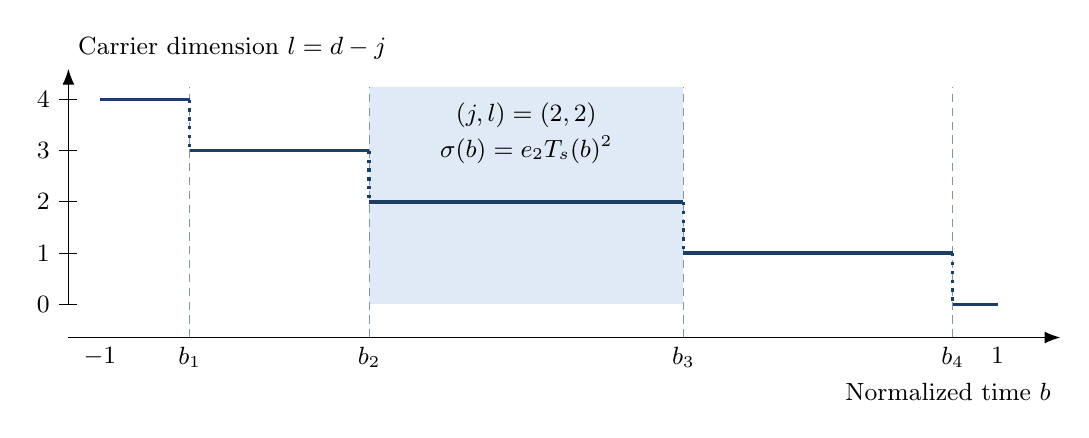
\begin{tikzpicture}[x=5.7cm,y=.65cm,font=\small,
  profile/.style={very thick,draw=linkblue},
  cut/.style={densely dashed,draw=linkblue!55}]
 \fill[figureblue] (-.4,0) rectangle (.3,4.25);
 \draw[-{Latex[length=2mm]}] (-1.07,0) -- (-1.07,4.6)
   node[above right] {Carrier dimension $l=d-j$};
 \foreach \l in {0,1,2,3,4}{
   \draw (-1.09,\l) -- (-1.05,\l);
   \node[left] at (-1.09,\l) {$\l$};
 }
 \foreach \b/\i in {-.8/1,-.4/2,.3/3,.9/4}{
   \draw[cut] (\b,-.65) -- (\b,4.25);
   \node[below] at (\b,-.65) {$b_\i$};
 }
 \draw[-{Latex[length=2mm]}] (-1.07,-.65) -- (1.14,-.65)
   node[below left,yshift=-13pt] {Normalized time $b$};
 \node[below] at (-1,-.65) {$-1$};
 \node[below] at (1,-.65) {$1$};
 \draw[profile] (-1,4) -- (-.8,4);
 \draw[profile] (-.8,3) -- (-.4,3);
 \draw[profile] (-.4,2) -- (.3,2);
 \draw[profile] (.3,1) -- (.9,1);
 \draw[profile] (.9,0) -- (1,0);
 \draw[profile,dotted] (-.8,4) -- (-.8,3);
 \draw[profile,dotted] (-.4,3) -- (-.4,2);
 \draw[profile,dotted] (.3,2) -- (.3,1);
 \draw[profile,dotted] (.9,1) -- (.9,0);
 \node[align=center] at (-.05,3.35)
   {$(j,l)=(2,2)$\\[2pt]$\sigma(b)=e_2T_s(b)^2$};
\end{tikzpicture}

\caption{An illustrative limiting profile in dimension four, with fixed
window width $s$ and cut times $(b_1,b_2,b_3,b_4)=(-0.8,-0.4,0.3,0.9)$.
The degree scales are $D_i=T_s(b_i)$, where $T_s(b)=B e^{bs}$, and
$e_j=\prod_{i\le j}D_i$. On the highlighted open plateau $(b_2,b_3)$,
two cuts have occurred and $\sigma(b)=e_2T_s(b)^2$.
The staircase shows carrier dimension; its vertical drops are schematic.
General profiles may have coincident limiting cuts.}
\label{fig:scale-profile}
\end{figure}
\FloatBarrier

\subsection{Testing individual components and products}

\begin{proposition}[Regularity and individual cuts]\label{prof:regularity}
Inside an open plateau, individual proper cuts of degree $O(T_s(b))$
on the different carriers collectively capture only $o(n)$ points.
At a slightly later interior testing time there are common equations
for the entire carrier family whose Jacobian has full codimension
rank at all but $o(n)$ points.  At those surviving points the carrier
is unique and smooth, and its tangent space is testable by equations
and minors of the same interior degree scale.

The assertions also hold for the union of two such families, and
for unions from $\exp(o(s))$ pieces with the same limiting profile
and width, provided each piece retains its own assigned masses.
Common equations vanish on the whole union.  In particular, two
different members of that union cannot meet at a surviving point
where the common Jacobian has full rank.
Flat carriers which are not defined over $\R$ may be discarded
with negligible mass.
\end{proposition}

\begin{proof}
Every carrier used here is an irreducible component of its fixed
path locus.  Indeed, at every point of the piece on that carrier,
the successive proper cuts give the current local dimension.  A
larger irreducible component containing the carrier would pass
through that point and contradict this local dimension.  The path
locus may have larger components elsewhere; they remain in its
equations.

Let the plateau start at time $\beta<b$, and choose
$b<b'<b''$ in the same plateau.  The carrier components are therefore
isolated components of their cut system, whose equations have degree
at most $B\exp((\beta+o(1))s)$.  Lemma~\ref{poly:pooling}, used at degree
$T_s(b')$, pools proper component cuts of degree $O(T_s(b))$ into
one polynomial.  It is nonidentically zero except on components of
total degree at most
\[
 e_j\exp(-(b'-b)s+o(s)).
\]
By~\eqref{prof:mass-budget} and $\prod_iD_i=N$, all points of the
piece touching those exceptional components have mass $o(n)$.
At every remaining counted point the pooled polynomial is proper
on every local carrier.  No-capture at $b'$ proves the assertion.

Apply Lemma~\ref{poly:regularity} at degree $T_s(b')$.  Since the
cut-system equations have degree at most $B\exp((\beta+o(1))s)$,
the components on which the common equations fail to have generic
full rank have total degree at most
\[
 e_j\exp(-(b'-\beta)s+o(s)).
\]
The mass budget removes all piece points touching those components
at a cost of $o(n)$.  On the other components a generic linear
combination of maximal minors is nonidentically zero.  Its zero set
contains every rank failure, and its degree is $O(T_s(b'))$.
The preceding individual-cut conclusion applies to this linear
combination using the remaining interior margin before $b''$, and
removes its zeros at another $o(n)$ points.  At a surviving point the
implicit function theorem gives a smooth locus of the correct dimension; any two
carrier components through that point would have the same germ
and hence would coincide.  The equations vanish on the whole
family, including components whose generic regularity failed.

For pooled pieces, use the union-of-systems versions of
Lemmas~\ref{poly:pooling} and~\ref{poly:regularity}.  Each carrier
remains a component of its own path system.  On a generic transverse
fiber, Lemma~\ref{poly:union-interpolation} interpolates the selected
isolated lists, including first jets, with an effective bound equal
to the sum of the individual system bounds: separators for the other
lists are multiplied, using their exact-isolation equations for a
test point outside a list.  If these bounds are $L_\nu$, then for
$\exp(o(s))$ pieces with the common limiting profile,
\[
 L_*=\sum_\nu L_\nu\le B\exp((\beta+o(1))s).
\]
The strict interior gaps above absorb this change in the effective
bound and the $\exp(o(s))$ changes in the degree budgets.

Mass accounting for such a union is performed separately in each
original piece.  Its own later cuts bound all of its points
touching exceptional components of its own current system.  We
do not apply one piece's later cuts to points assigned to another
piece.  Rank failures on every good assigned component are then
discarded by that piece's no-capture assertion.  The equations
still vanish on the whole union, so full rank at a surviving point
also excludes intersections with a carrier from another piece.
The sequence quantifier makes the discarded fractions uniform
over these pieces; summing their masses creates no loss equal to
the number of pieces.

Finally, the real points of a nonreal complex affine flat lie in
a proper complex affine linear section of that flat.  Choose
one such degree-one proper cut for each nonreal flat, and no
cut on the other carriers.  The individual-cut assertion just
proved makes their total assigned mass negligible.
\end{proof}

For the next lemma, write $S_x,S_y$ for the two point sets and
$n_x=|S_x|$, $n_y=|S_y|$.  A dense graph is a subset
$\Gamma\subset S_x\times S_y$ of size at least $\alpha n_xn_y$
for some fixed $\alpha>0$.  A label map is a rational map $\phi$
from pairs to a fixed affine space, with bounded-degree coordinate
numerators and denominators on the chosen charts.  The image assigned
to carriers $X,Y$ is the closure of $\phi(X\times Y)$.

\begin{lemma}[Product testing]\label{prof:product-testing}
Take two pieces, or the pooled pieces described above, in a common
window with the same limiting profile. On a fixed plateau, fix in
each set an assignment of every point to one carrier of its original
piece that contains it. These assignments precede the tests below
and are retained under later restrictions. Let $X,Y$ denote the
assigned carriers of a pair, and fix an interior testing time $b$.
A polynomial of degree $O(T_s(b))$ captures only
$o(n_xn_y)$ pairs at which it does not vanish identically on
$X\times Y$. The same holds for a number of rational tests bounded
independently of the sequence, provided their denominators are
nonzero at the pairs concerned and their numerator polynomials have
degree $O(T_s(b))$ on the chosen charts, with a common implied
constant.

Consequently an equation system containing the labels of a dense
graph contains the complete assigned component images at all but
a negligible fraction of its pairs, whenever the label map has
bounded degree on these charts and the cleared numerator polynomials
of all pulled-back equations have degree $O(T_s(b))$ with a common
implied constant. The denominators used in these pullbacks must be
nonzero at the actual pairs concerned. For any collection of rational
rank tests whose size is bounded independently of the sequence and
which are generically nonzero on the relevant assigned images, the
tests are nonzero at all but $o(n_xn_y)$ corresponding actual pairs,
provided their denominators are nonzero there and their cleared
pullback numerators obey the same degree bound.
\end{lemma}

\begin{proof}
For an actual source point $p$, apply the individual-cut conclusion
of Proposition~\ref{prof:regularity} on every target carrier $Y$
on which the specialization is nonidentically zero.
For the other case, fix $Y$.  If the polynomial is not identically
zero on $X\times Y$, choose a generic $y\in Y$ for which its
specialization is nonidentically zero on each such $X$.
The same individual-cut conclusion on the source bounds points $p$ where the polynomial vanishes
identically on $Y$.  Average this bound with the target masses of
the $Y$'s. The fixed assigned sets are disjoint within each factor,
so these weighted sums are unambiguous even when carriers meet.
For pooled pieces, retain their original mass accounting.
All bounds are uniform over the polynomial and the
pieces by their sequence formulation.

For a system of equations, pull back each equation and clear its
chart denominator separately. The resulting numerator polynomials
vanish at the actual system points and have the common degree bound.
On every component product carrying a pair on the chart whose image
is not contained in the system, at least one numerator is
nonidentically zero. A generic linear combination of the numerators
is therefore nonidentically zero on every such product
simultaneously. It has the same degree bound: a finite basis of
their span suffices, regardless of the number of system equations.
Apply the first assertion to this combination.

For rank tests use their cleared pullback numerators. When a rank
condition is expressed by minors whose cleared numerators obey the
common degree bound, a generic linear combination of those numerators
is nonidentically zero on every relevant component product where the
rank condition holds generically, and its zero set contains every
rank failure. A bounded number of the resulting
tests has a union of failure sets of size $o(n_xn_y)$. A slightly
later interior time absorbs the uniform constant in the degree
bound. This proves the last assertion without assuming that sample
points are generic on their carriers.
\end{proof}

\subsection{Selecting the two windows}

\begin{proposition}[Selection of profile pairs]\label{prof:pair-selection}
For every $p\in P$, let $C_p$ be a finite family of irreducible
projective curves in $\PP^{d-1}$, each spanning a projective subspace
of dimension at most two, with total degree at most $E=\delta N/A$.
Suppose that $1-o(1)$ of
the unordered pairs $\{p,q\}$ satisfy $\pi_p(q)\in C_p$ or
$\pi_q(p)\in C_q$.  After the global terminal deletion described
below, one of the following configurations occurs.
\begin{enumerate}
\item A core of positive relative size is covered.
\item Two sequences of non-core pieces have a common dyadic width
$s$, the same limiting profile, and an ordered product covered in
one orientation with positive relative density.
\item Two sequences of non-core pieces have widths with ratio
tending to infinity, both $o(\log B)$, the same limiting profile,
and such a positively covered ordered product.
\end{enumerate}
In the common outermost window $s=\log B$, the two factors may
instead be the same pool of pieces in a shrinking profile bin.
That pool has size $n\ge N\sqrt\delta$, is the union of
$\exp(o(s))$ pieces, and retains all the preceding degree, mass,
regularity, and product-testing conclusions to exponential
accuracy.  All selected incidences may be required to lie on
physical lines containing at most $B^{o(1)}$ sample points.

The global terminal deletion means the following.  Whenever a
target point was assigned to its carrier curve after the
$(d-1)$st cut, its projection from the center is not a curve
contained in the center's directional family.
\end{proposition}

\begin{proof}
Assign each point of every non-core piece to one of its carrier
curves after the $(d-1)$st cut.  Omit assignments to nonreal lines.
Such a line contains at most one real point, so the omitted
fraction in a piece is at most
\[
 \frac{e_{d-1}\exp(o(s))}{n}
 =D_d^{-1}\exp(o(s))=o(1),
\]
using~\eqref{prof:balance}.  This is uniform over pieces.  Every
point is assigned at most once; pool repeated curves.  Apply
Proposition~\ref{geo:terminal} once to this global assignment.  It removes
only $o(N^2)$ ordered incidences, and hence leaves the required
almost-complete unoriented coverage.  Assignments retain their
original meaning if pieces are later pooled.

If the core has positive relative size, the cone over a
directional family has degree $O(E)$ and dimension at most two.
The core's isolation equations, restricted to its components,
and B\'ezout bound its intersections with the core by $O(EL^2)$
per center.  This is $o(N)$, so neither orientation can cover a
positive fraction of the core pairs.  This resolves the first
alternative.  Otherwise discard the core.

Here are details of the remaining selection, including the order
of the limits.  First fix a precision $1/h$, and partition the
compact space of normalized drop lists and values of
$s/\log B\in[0,1]$ into finitely many bins of that diameter.
Also bin the dyadic index modulo an integer tending to infinity
with $h$.  Two independent random retained points fall in one
common bin with probability bounded below by a positive constant
depending only on $h$.  Thus the relative uncovered probability
conditional on this agreement tends to zero for fixed $h$.
Select a pair of pieces with small relative uncovered
probability, and pass to an orientation containing at least half
the covered pairs.  Now let $h$ tend to infinity sufficiently
slowly with the sample index.  This standard diagonal choice
retains conditional coverage while making the profiles and
normalized widths converge to the same limits.

The selected dyadic indices are either equal on a subsequence,
or their difference tends to infinity, by their congruence
condition.  In the latter case the width ratio tends to infinity.
Their normalized widths have the same limit, so that limit must
be zero.  This proves the two window alternatives.

There is a useful refinement at the outermost window.  If its
total mass tends to zero, discard it before the selection.  If
its mass is bounded below on a subsequence, work only there.
For each fixed precision choose a largest profile bin and use
its pool as both factors.  It has a fixed positive mass at that
precision, and its relative uncovered fraction tends to zero.
In the diagonal choice increase precision slowly enough that
its mass is at least $N\sqrt\delta$ and
$N\exp(-o(\log B))$.  This is possible because $\delta\to0$.
Each constituent piece has size $N\exp(-o(s))$ uniformly, so
there are only $\exp(o(s))$ of them.  Their profiles differ by
$o(1)$, and the conclusions for pooled families follow from
Proposition~\ref{prof:regularity} and
Lemma~\ref{prof:product-testing}.

Finally, Szemer\'edi--Trotter, with a generic planar projection,
makes the fraction of ordered pairs on lines of occupancy above
a threshold $H$ arbitrarily small as $H\to\infty$: summing its
dyadic rich-line estimate gives $O(N^2/H+N h_{\max})$, and the
proper-flat bound gives $h_{\max}=o(N)$.  At each fixed selection
precision first choose $H$ large enough for its conditioning
probability.  Increase the precision sufficiently slowly that
$H\le B^{o(1)}$ and all the preceding conditional errors still
vanish.  This is compatible with the outer-pool mass condition.
All constants and precisions are fixed before taking each
asymptotic limit; the final diagonal sequence merely combines
these finitely specified requirements.
\end{proof}

\section{The sparse-cones assertion}\label{sec:sparse-cones}

We retain the contradiction hypotheses, including the
lower-dimensional induction bounds and their proper-flat
consequences.  For $p\in\R^d$ and $y\ne p$, write $\pi_p(y)=[y-p]$.
A directional curve family is a finite family of curves in
$\PP^{d-1}$; membership means membership in its union, and its
total degree is the sum of the component degrees.

\begin{theorem}[Sparse cones]\label{sc:theorem}
Along a sequence with $M=o(A)$, there cannot be families $C_p$,
one for each $p\in P$, of irreducible projective curves, each
spanning projective dimension at most two, such that
\[
 \deg C_p\le E=\delta N/A,\qquad \delta\to0,
\]
and $1-o(1)$ of the unordered pairs $\{p,q\}$ satisfy
$\pi_p(q)\in C_p$ or $\pi_q(p)\in C_q$.
\end{theorem}

Suppose these data exist. Apply the results of Section~\ref{sec:profiles}.
The positive-mass core alternative is already contradictory.
We must treat a common window and two widely separated windows.
The selected covered incidences retain the global terminal deletion and
the light-line restriction in Proposition~\ref{prof:pair-selection}.
For the common-window rank estimate we will also use auxiliary graphs
of arbitrary ordered pairs $(p,q)$ with $p\ne q$ on the same selected point sets.
That estimate will be proved without a coverage or light-line hypothesis.

We use affine charts of the label map
\begin{equation}\label{sc:label-map}
 \psi(x,y)=(x,\pi_x(y)).
\end{equation}
For each finite family under discussion, these charts may be chosen to
contain all actual labels and to meet every component image.
The map and its pullbacks have bounded degree on these charts;
constant factors in testing degree fit inside a chosen open
plateau.  A \emph{dense graph} means at least a fixed positive
fraction of the ordered product of the two selected pieces.
Assertions about dense graphs always include arbitrary further
fixed positive-density restrictions and subsequences.

\subsection{Product images and rank in a common window}

Consider two pieces with width $s$ and the same limiting profile,
or the outermost pool allowed by Proposition~\ref{prof:pair-selection}.
Use $D_i,e_j,\sigma$ from~\eqref{prof:profile-functions}.
For an ordered graph $\Gamma$ on these pieces, write
$H(T)=H_{\psi(\Gamma)}(T)$ for the restriction rank of its labels.

We first make the passage from carrier pairs to product images precise.
The same construction will be used in the rank argument and, with one
fixed choice of parameters, at the outermost endpoint.  Its last estimate
applies to every later choice of image subfamily.

\begin{lemma}[Retained products and their image degree]
\label{sc:retained-products}
Fix a common positive-dimensional plateau after $j$ cuts, of dimension
$k=d-j<d-1$, and choose an interior time $\tau$ on that plateau.  Write
$n_x,n_y$ for the original source and target counts.  Given a fixed
$\varepsilon>0$, one may discard $o(n_x)$ source points and
$o(n_y)$ target points.  Write $m_x,m_y$ for the remaining counts, so
$m_x=(1-o(1))n_x$ and $m_y=(1-o(1))n_y$.  One may then discard carrier
pairs of total assigned product mass $o(m_xm_y)$, with the following conclusions.

Each remaining point is assigned to its unique smooth carrier in the
union of the two physical families.  Repeated carriers are pooled within
each family, and every flat carrier with positive assigned mass is real.
There are common physical equations for the whole original union whose Jacobian
has full codimension rank at these points.  A single polynomial
$g_{\rm ph}$, a linear combination of maximal Jacobian minors, is nonzero
at every retained point.  The equations and this test have degrees
$O(T_s(\tau))$.
When the two factors are the same pool, the point deletion and the
assignment may be taken to be the same in both roles.

Write $\mathcal R$ for the retained ordered carrier pairs and
\[
 Z_{X,Y}=\overline{\psi(X\times Y)}\qquad((X,Y)\in\mathcal R).
\]
Every $Z_{X,Y}$ has dimension $2k$, and at a general pair the connecting
direction is transverse to both physical tangent spaces.  Let $U$ be the
reduced union of the distinct $Z_{X,Y}$.  Then
\begin{equation}\label{sc:retained-image-upper}
 \deg U\le e_j^2\exp(o(s)).
\end{equation}
For any subfamily $\mathcal J$ of these distinct images, including one
chosen after further equations have been chosen, its represented carrier
pairs have normalized assigned mass at most
\begin{equation}\label{sc:retained-image-mass}
 \frac{1}{m_xm_y}
 \sum_{\substack{(X,Y)\in\mathcal R\\Z_{X,Y}\in\mathcal J}}n_Xn_Y
 \le \frac{\deg\bigl(\bigcup_{Z\in\mathcal J}Z\bigr)}{e_j^2}
       \exp(\varepsilon s+o(s)).
\end{equation}
Here $n_X,n_Y$ are the assigned masses after the point deletions.
\end{lemma}

\begin{proof}
Choose fixed times $\tau_{\rm eq}<\tau_{\rm test}<\tau$ between the start
of the plateau and $\tau$.  Use the earlier part of this interval for
the equation choices in Proposition~\ref{prof:regularity}, leaving the
strict gap up to $\tau_{\rm test}$ for its minor and proper-cut tests at
the sample points.  Apply its union version to the two physical carrier families.
It removes the negligible point sets excluded by its regularity conclusion
and supplies common equations for the whole union.  At each remaining
point there is now a unique smooth carrier.  Denote by $g_{\rm ph}$ the
common combination of maximal minors whose zeros were removed in this
step.  Discard every such point
whose carrier is a nonreal flat, using the degree-one proper sections in
the last paragraph of that proposition.  This costs another
$o(n_x)+o(n_y)$ points.  The source and target assignments are now
unambiguous.  Each assigned carrier belongs to the point's own original
piece path: that path already supplies a carrier through the point, and
uniqueness in the full union identifies it with the assigned member.
For two copies of the same pool take the union of the two negligible
point deletions in both roles; the resulting assignment is the same.
Extend the retained assignments by assigning each deleted point to a
containing carrier of its original piece before any later product tests,
using the same extension in both roles for a common pool.  Product testing
on the original sets then retains the present assignments under restriction, and its
$o(n_xn_y)$ pair loss is also $o(m_xm_y)$.  Pool equal retained carriers
within each of the two lists and omit members with zero mass.
All these choices have been made inside the interval ending at $\tau$,
which gives the stated degree bound.

The pooled budgets, with each original piece still supplying the bound
for its own points, give
\begin{equation}\label{sc:retained-carrier-weights}
 \begin{gathered}
 \max\left\{\sum_X\deg X,\sum_Y\deg Y\right\}\le e_j\exp(o(s)),\\
 \frac{n_X}{m_x}\le\frac{\deg X}{e_j}\exp(o(s)),\qquad
 \frac{n_Y}{m_y}\le\frac{\deg Y}{e_j}\exp(o(s)).
 \end{gathered}
\end{equation}
Indeed, the mass of a carrier in one piece is at most
$\deg(X)(N/e_j)\exp(o(s))$, and pooling $\exp(o(s))$ pieces changes
this by only $\exp(o(s))$.  The remaining point counts are still
$N\exp(-o(s))$.  A flat has degree one, so its number and its normalized
weight satisfy the hypotheses of Lemma~\ref{geo:generic-depth} with
$w=s$ and $e=e_j$.  The flat members are real by the preceding deletion.

Apply that lemma now with the fixed $\varepsilon$.  Let
$\mathcal Y_X$ be its target list for $X$, and set
$\mathcal R=\{(X,Y):Y\in\mathcal Y_X\}$.  The removed carrier pairs
have normalized product weight $o(1)$, hence account for $o(m_xm_y)$
actual pairs.  This deletion includes pairs generically tangent at either
endpoint.  Thus the target tangent projects injectively at a general pair,
and the first coordinate of $\psi$ records all source tangent directions;
the product image has dimension $2k$.  The preimages of a general
$2k$-fold linear section of that image are isolated away from the base
locus of the bounded-degree map on $X\times Y$.  The isolated-intersection
form of B\'ezout therefore gives
$\deg Z_{X,Y}\le C_d\deg X\deg Y$, and
\eqref{sc:retained-image-upper} follows from
\eqref{sc:retained-carrier-weights}.

We prove the uniform subfamily estimate while keeping these same lists.
Images belonging to different source carriers are distinct: the closure
of the first projection of $Z_{X,Y}$ is $X$.  Fix one source $X$ and one
of its distinct images $Z$.  To identify its source fibers, take its
closure $\widehat Z\subset X\times\PP^{d-1}$ before restricting the
direction coordinate to our affine chart.  Localizing the ideal of the
rational image at $\C(X)$ identifies the generic fiber with the closure
of the projection of $Y$ from the generic source point.  This fiber is
geometrically integral, since it is the image closure of the geometrically
integral variety $Y_{\C(X)}$.  After restricting $X$ to a dense open,
the projective family is flat with geometrically integral fibers of a
constant degree $d_Z$; this uses generic flatness, geometric integrality after
shrinking, and constancy of the Hilbert polynomial in a flat projective
family \cite[Tags~052A, 0559, 0C0E, and 0B9T]{stacksproject}.
We may also require that projection of $Y$ from each $x$ in this open set
has dimension $k$, by generic target transversality.
Its closed image is then a $k$-dimensional irreducible subvariety of the
$k$-dimensional integral fiber, so it equals the whole fiber.  Make these
restrictions simultaneously for the finite image and target lists.
Thus all targets with $Z_{X,Y}=Z$ have the same complete projected image
at a common general $x\in X$.  Write $t_x(Y)$ for their generic map degrees.
The fixed list bound says
\[
 \sum_{Y:\,(X,Y)\in\mathcal R,\ Z_{X,Y}=Z}t_x(Y)
 \le \exp(\varepsilon s).
\]
For a general $x$, the point-projection formula gives
$\deg Y-\operatorname{mult}_xY=t_x(Y)d_Z$.
The multiplicity is zero unless $X=Y$.  In that case $x$ is smooth and
the multiplicity is one; a coincident flat pair was deleted as tangential.
Consequently $\deg Y\le2t_x(Y)d_Z$ for every target in this sum.

Choose $k$ general affine hyperplanes in the source coordinates.  They
meet $X$ in $\deg X$ points of the preceding open set.  Then choose $k$
general hyperplanes in the direction coordinates; on each complete fiber
they give $d_Z$ points, with multiplicity.  The choices can be made so
all these points lie in the selected label chart and avoid intersections
between distinct images.  The resulting mixed section of $Z$ therefore
has $\deg X\,d_Z$ points.  The $2k$ blockwise hyperplanes are also affine
linear equations in the full label space.  Their homogenizations restrict
to linear equations on the ordinary projective closure of $Z$, where all
the counted affine points are isolated intersections.  The isolated-intersection
form of B\'ezout bounds their total multiplicity by the ordinary degree,
even if the same equations have additional components at infinity.
Applying this to a reduced image subfamily and summing the preceding
map-degree bound gives
\[
 \sum_{\substack{(X,Y)\in\mathcal R\\Z_{X,Y}\in\mathcal J}}
       \deg X\deg Y
 \le C_d\exp(\varepsilon s)
       \deg\bigl(\bigcup_{Z\in\mathcal J}Z\bigr).
\]
Multiplying the two weight bounds in
\eqref{sc:retained-carrier-weights} proves
\eqref{sc:retained-image-mass}.  No further generic-depth deletion is
made when $\mathcal J$ is chosen.
\end{proof}

\begin{lemma}[Common-window label rank]\label{sc:common-rank}
Let $\Gamma\subset\{(p,q)\in S_x\times S_y:p\ne q\}$ be any dense graph
on the selected pieces or pool; its pairs need not be covered by the $C_p$.
For its labels, at an interior testing time
before the last cut,
\begin{equation}\label{sc:label-rank}
 H(T_s(b))\ge
 \sigma(b)^2\min\left(1,\frac{T_s(b)}{D_1D_2}\right)
 \exp(-o(s)).
\end{equation}
The convention is a lower limit after dividing the logarithm
by $s$; in particular it permits any prescribed fixed positive
logarithmic tolerance, uniformly for dense subgraphs.
\end{lemma}

\begin{proof}
On the initial full-dimensional interval,
Lemma~\ref{prof:product-testing}, or its two successive
full-dimensional no-capture arguments, forces the testing-degree
envelope of a dense label graph to be the whole label space.
Its rank is comparable to $T^{2d-1}$.  Since $D_1D_2\ge T^2$
there, this is at least the right side of~\eqref{sc:label-rank}.

On a positive-dimensional plateau after $j\ge1$ cuts put
$k=d-j$.  Choose a physical regularity time between the start of this
plateau and the current testing time $b$.
When $k<d-1$, apply Lemma~\ref{sc:retained-products} with any fixed
$\varepsilon>0$.  When $k=d-1$, apply
Proposition~\ref{prof:regularity} to the union of the two physical
families, discard its rank-failure and nonreal-flat points, and assign each
survivor to its unique carrier from its original path.  Use the same
supported extension to the original point sets before product testing,
and pool equal retained carriers with their assigned masses.  The fixed
tangent-flat argument and the proper-flat
cap then discard carrier pairs generically tangent at either endpoint.
In both cases the point and carrier-pair losses remove only a negligible
fraction of the graph, and every remaining complete product image
$\overline{\psi(X\times Y)}$ has dimension $2k$.
Product testing forces these complete images into the testing-degree
envelope at almost all remaining graph pairs.

For this fixed envelope, choose one irreducible envelope component
containing each distinct complete image occurring at those surviving
pairs.  Let the pairs with that image inherit its choice.  Group all
envelope components by dimension and count each surviving pair in the
group of its chosen component; components receiving no pairs remain in
the degree of their group.  Every chosen component has dimension at
least $2k$, so some dimension $h\ge2k$ group carries a positive
fraction of the graph.  Write $a$ for its degree and $\Gamma'$ for
the graph portion it carries.

If $h\ge2k+1$, the Hilbert bounds give
\[
 H(T)\gtrsim aT^h,\qquad
 H_{\psi(\Gamma')}(T')\lesssim a(T'+1)^h.
\]
Borrow~\eqref{sc:label-rank} from a time just before the cut
starting this plateau.  The required right side grows with
exponent at most $2k+1$ within the plateau, so growth with
exponent $h$ suffices.  Endpoint approximation costs an
arbitrarily small fixed multiple of $s$ in the logarithm.

It remains to bound $a$ when $h=2k$.  Each image assigned to this group
is an irreducible $2k$-fold contained in its chosen irreducible
$2k$-dimensional envelope component, and therefore equals that component.
If $k=d-1$, necessarily $j=1$, and the projection of a generic
target hypersurface from a generic source point fills direction
space.  For each source carrier $X$ the product image is thus
$X\times\PP^{d-1}$ in these label coordinates.  A positive
mass of pairs requires a positive source mass.  The carrier
mass budget therefore gives
\[
 a\gtrsim e_1\exp(-o(s))=D_1\exp(-o(s)).
\]
The resulting rank $D_1T^{2d-2}\exp(-o(s))$ is sufficient:
on this plateau $T\le D_2$ to exponential accuracy and
\[
 D_1^2T^{2d-2}\min(1,T/(D_1D_2))
 \le D_1T^{2d-2}.
\]

Now suppose $k<d-1$.  The images assigned to this group represent
a positive amount of assigned product mass, since they carry
$\Gamma'$.  Apply \eqref{sc:retained-image-mass} to this subfamily.
Its degree is at most $a$, so
\[
 a\gtrsim e_j^2\exp(-\varepsilon s-o(s)).
\]
Since $\varepsilon$ is arbitrary, $a\ge e_j^2\exp(-o(s))$.
The Hilbert lower bound now gives $H(T)\ge e_j^2T^{2k}\exp(-o(s))$,
which is stronger than~\eqref{sc:label-rank} on this plateau.

These alternatives propagate through the finitely many distinct
cut times.  If the first boundary has degree $\exp(o(s))$ and
there is no earlier testing time of degree at least one, use
rank one there; the required boundary value is itself
$\exp(o(s))$.  This also handles several simultaneous first
cuts.  Every borrowed graph portion has fixed positive density
after passage to a subsequence, so the induction applies to it
as asserted.
\end{proof}

The graph covered in the selected orientation has an independent
upper bound, obtained by specializing at each actual center:
\begin{equation}\label{sc:common-upper}
 H(T)\le CNE(T+1).
\end{equation}
Near the last cut, $\sigma(b)$ is $N$ within an arbitrarily
small logarithmic tolerance.  Comparing
\eqref{sc:label-rank} and~\eqref{sc:common-upper}, the relevant
ratio is, to the same accuracy, at least
\begin{equation}\label{sc:common-ratio}
 \min\left(\frac{A}{\delta D_d},
            \frac{A}{\delta D_1D_2}\right).
\end{equation}
The second term has a strict positive $s$-scale margin because
$b_1+b_2<0$.  The first does also unless $s=\log B$ and $b_d=1$:
if the common window is not outermost, $s\le\tfrac12\log B$,
whereas in the outermost window its margin is $1-b_d$.
Choosing a fixed testing time sufficiently close to the final
cut therefore gives a contradiction in every other case.
No comparison between $\delta$ and an uncontrolled
$\exp(o(s))$ factor has been made.

\subsection{The outermost endpoint}

Assume now $s=\log B$ and $b_d=1$.  Use the common pool supplied by
Proposition~\ref{prof:pair-selection}; initially its size $n_0$ satisfies
\begin{equation}\label{sc:outer-pool}
 n_0\ge N\sqrt\delta,\qquad n_0=N\exp(-o(s)).
\end{equation}
Let $\Gamma_0$ be its graph covered in the selected orientation.  It has
at least $\alpha n_0^2$ pairs for a fixed $\alpha>0$, and retains the
terminal deletion and the light-line restriction.  Let $k$ be the
dimension of the final open plateau, $j=d-k$, and let $\beta=b_j<1$
be its starting time.  Balance gives
\begin{equation}\label{sc:outer-budgets}
 1\le k<d-1,\qquad e_j=B^{d-2k},\qquad N/e_j=A^k.
\end{equation}

At this endpoint the rank comparison can have zero logarithmic margin.
We will instead lift the covering direction curves to physical curves.
For this, we need one fixed family of product images and one common
smooth system containing the images used by all the lifts.

Choose fixed interior times
\begin{equation}\label{sc:outer-time-choice}
 \beta<\tau<t_0<t_1<t_2<1,
 \qquad t_0>\max\{\beta,1+b_1+b_2\}.
\end{equation}
Such choices exist because $b_1+b_2<0$.  Reserve the interval
$(\beta,\tau)$ for the finitely many physical regularity choices,
use $t_0$ for the image envelope and $t_1$ for the common label equations,
and reserve $(t_1,t_2)$ for the later pullback tests.  Now fix
\[
 0<\varepsilon<\tfrac14(t_1-t_0).
\]
Also fix the endpoint approximation and the logarithmic tolerances in
the rank argument below smaller than a quarter of both positive gaps
$t_0-\beta$ and $t_0-(1+b_1+b_2)$.

Apply Lemma~\ref{sc:retained-products} to the two copies of this pool,
with $\tau$ and $\varepsilon$ just fixed.  Use its same-pool deletion
and assignment, and retain its common physical equations and
$g_{\rm ph}$ for the full original union of final-plateau carriers.

When $k\ge2$, make one further point deletion before fixing the final
product family.  The carriers whose affine spans have dimension at most
$k+1$ number at most $e_j\exp(o(s))$, and each lies in a proper flat
containing at most $B^{k+1+o(1)}$ sample points.  The points assigned to
all these carriers therefore have total mass at most
\[
 B^{d-2k}B^{k+1+o(1)}=B^{d-k+1+o(1)}=o(n_0).
\]
Discard them in both roles.  No such deletion is made when $k=1$.

Write $S$ for the resulting pool, $n=|S|$, and $\mathcal C$ for its
positive-mass physical carriers.  Then
\begin{equation}\label{sc:outer-retained-pool}
 n=(1-o(1))n_0\ge(1-o(1))N\sqrt\delta,
 \qquad n=N\exp(-o(s)).
\end{equation}
Restrict the returned carrier pairs to $\mathcal C\times\mathcal C$
and call this fixed set $\mathcal R$.  Its omitted assigned product mass
is still $o(n^2)$.  The old assigned weights only decreased in the last
point deletion, while the normalizing point count changed by a factor
$1-o(1)$.  Thus \eqref{sc:retained-image-mass} remains valid, with the
same $\varepsilon$ and an adjusted $o(s)$, for every subfamily of the
distinct images
\[
 Z_{X,Y}=\overline{\psi(X\times Y)},\qquad (X,Y)\in\mathcal R.
\]
Let $U$ be their reduced union.  This is the final product-image family
for this endpoint; we will only take subfamilies of it.  In particular
$\deg U\le e_j^2\exp(o(s))$.  Restrict $\Gamma_0$ to $S\times S$ and
to the carrier pairs in $\mathcal R$, and call the result $\Gamma$.
The point and carrier-pair deletions together cost $o(n_0^2)$ pairs, so
$|\Gamma|\gtrsim n^2$.

When $k=1$, the unique carrier of each surviving target is its globally
assigned terminal curve from Proposition~\ref{prof:pair-selection}.
Indeed, the final plateau is then after the $(d-1)$st cut.  The curve
chosen in that global assignment belongs to the full original carrier
union used by the common physical equations, so uniqueness at the target
identifies it with the current carrier.  If that global assignment was
omitted because its chosen curve was a nonreal line, uniqueness would
make the current carrier that line, and the nonreal-flat point deletion
has removed the point.  Thus no globally unassigned target remains in
this case.

\begin{lemma}[Regular product images at the endpoint]
\label{sc:outer-regularity}
For the fixed $\mathcal R$ and $U$ above, there is a subfamily
$\mathcal R_{\rm sm}\subseteq\mathcal R$ whose omitted assigned product
mass is $o(n^2)$, and one system of label equations of degree at most
$B^{2-c}$ for some fixed $c>0$, with the following properties.
The equations contain every complete image $Z_{X,Y}$ for
$(X,Y)\in\mathcal R_{\rm sm}$.  Outside $o(n^2)$ further actual pairs
assigned to $\mathcal R_{\rm sm}$, their common zero locus is smooth of
dimension $2k$ at the label, the product map has differential rank
$2k$, and the connecting direction is transverse to both physical
tangent spaces.  If $k\ge2$, the two projected tangent spaces are also
unequal there.  The equations and every polynomial test used for these
actual-pair conclusions have degree at most $B^{2-c}$.
\end{lemma}

\begin{proof}
Put $T_i=T_s(t_i)$ and form
\[
 V=\operatorname{Env}_{T_0}(U).
\]
For each distinct image $Z\subset U$, choose once an irreducible component
$W(Z)$ of $V$ containing the whole image.  Every assigned pair represented
by $Z$ inherits that choice.  Since $\dim Z=2k$, a chosen component has
dimension at least $2k$; equality implies $W(Z)=Z$.

We first show that the images assigned to larger components represent
only $o(n^2)$ product mass.  Otherwise, after taking a subsequence, some
dimension $h\ge2k+1$ group represents a fixed positive normalized mass.
Form an auxiliary graph $\Lambda_h$ from all actual ordered pairs in
those assigned products, omitting the diagonal where $\psi$ is undefined.
Disjointness of the assignments makes its size equal to that product
mass before the omission, and the diagonal has at most $n$ pairs.
Thus $\Lambda_h$ is dense in $S\times S$.  This graph is independent of
the covered graph $\Gamma$; the arbitrary-graph scope of
Lemma~\ref{sc:common-rank} applies to it.
Every label of $\Lambda_h$ lies in the chosen dimension-$h$ component
containing its complete product image.

Write $a_h$ for the total degree of the dimension-$h$ component group of
$V$, including components receiving no images.  Its upper Hilbert bound
at an earlier degree $T'$ controls $H_{\psi(\Lambda_h)}(T')$, while its
lower envelope bound gives $H_V(T_0)\gtrsim a_hT_0^h$.  Borrow the
common-window label rank at a time just before $\beta$, with the fixed
endpoint tolerance chosen above.  If $\beta=-1$ and no earlier testing
degree is at least one, use the rank-one boundary convention in
Lemma~\ref{sc:common-rank}; then all $j$ earlier cut times equal $-1$
and the required boundary rank is one to exponential accuracy.
On the final plateau $\sigma(b)=e_jT_s(b)^k$.  Propagating with
$h\ge2k+1$ therefore gives
\[
 H_V(T_0)\ge e_j^2T_0^{2k}
 \min\left\{\frac{T_0}{T_s(\beta)},
             \frac{T_0}{D_1D_2}\right\}
       \exp(-\xi s-o(s)),
\]
where the fixed $\xi>0$ can be smaller than both gaps specified after
\eqref{sc:outer-time-choice}.  The two factors have normalized logarithms
$t_0-\beta$ and $t_0-(1+b_1+b_2)$, respectively, so the lower bound has
a strict positive margin.  But envelope equality and the upper Hilbert
bound on the pure $2k$-dimensional family $U$ give
\[
 H_V(T_0)=H_U(T_0)\le C e_j^2T_0^{2k}\exp(o(s)).
\]
This contradiction proves the claimed product-mass deletion.

Let $\mathcal I$ be the distinct images left after that deletion.
Each is an actual irreducible $2k$-dimensional component of the single
locus $V$, defined by equations of degree at most $T_0$; larger components
elsewhere in $V$ are kept in those equations.  Also
$\deg\mathcal I\le\deg U\le e_j^2\exp(o(s))$.
Apply Lemma~\ref{poly:regularity} to this pure component family at degree
$T_1$.  Its equations vanish on the whole family $\mathcal I$.
The exceptional image subfamily $\mathcal E$ has total degree at most
\[
 C\deg(\mathcal I)\frac{T_0}{T_1}
 \le e_j^2\exp(-(t_1-t_0)s+o(s)).
\]
Use \eqref{sc:retained-image-mass} for this particular subfamily of the
already fixed $U$.  Its represented normalized pair mass is at most
\[
 \exp(-(t_1-t_0-\varepsilon)s+o(s))=o(1).
\]
Here the same $\varepsilon$-lists chosen before $U$ are used; no new
generic-depth deletion depends on $\mathcal E$.  Let
$\mathcal R_{\rm sm}$ consist of the carrier pairs represented by
$\mathcal I\setminus\mathcal E$.  The two image deletions have omitted
only $o(n^2)$ assigned product mass.

The regularity lemma supplies a common polynomial $g$ of degree $O(T_1)$,
a linear combination of maximal Jacobian minors, which is nonzero on each
image in $\mathcal I\setminus\mathcal E$.  The single rational pullback
$g\circ\psi$ has a cleared numerator of degree $O(T_1)$ on the chosen
charts, nonidentically zero on every carrier pair in $\mathcal R_{\rm sm}$.
Product testing, with its
internal times in $(t_1,t_2)$, removes its actual zeros at a cost of
$o(n^2)$ pairs.  At every surviving label the common equations are locally
a smooth $2k$-fold.  They still vanish on all of $\mathcal I$, including
its exceptional components.

It remains to test the two tangent injectivities at actual pairs.
Write $f_a$ for the common physical equations chosen before $\tau$, and
$v=q-p$.  At a point $r\in S$, their Jacobian has kernel $T_r$, the tangent
space of its unique carrier.  Thus $v\notin T_r$ exactly when at least one
polynomial $\nabla f_a(r)\mathbin{\cdot}v$ is nonzero.  These tests have
degree $O(T_s(\tau))$ in $(p,q)$.  On every retained carrier pair the
source collection and the target collection each contain a generically
nonzero test, by the fixed generic-depth deletion.  For each endpoint,
choose a generic constant linear combination nonzero on every retained
product.  Product testing removes its actual zeros at cost $o(n^2)$.
The target injectivity, together with the source coordinate of $\psi$,
gives differential rank $2k$; the source injectivity is retained
separately for the secant step.

If $k\ge2$, every remaining physical carrier spans dimension at least
$k+2$ by the preceding carrier deletion.  Equality of the two projected tangent
spaces at a general retained pair would put both carriers in a common
$(k+1)$-flat by Lemma~\ref{geo:secants}, which is impossible.  This
inequality also has a bounded-degree test using the same physical
equations.  Put $c'=d-k$ and write $a_i(r)=\nabla f_i(r)$.  On the
full-rank transverse locus the row vectors
\[
 (a_i(r)\mathbin{\cdot}v)a_j(r)
 -(a_j(r)\mathbin{\cdot}v)a_i(r)
\]
span the $(c'-1)$-dimensional annihilator of $T_r+\mathbb Cv$.
Indeed, they lie in that annihilator, and choosing one row with nonzero
value on $v$ expresses every row combination annihilating $v$ in their
span.  The two projected tangent spaces are unequal exactly when the
combined row spans for $r=p,q$ have rank at least $c'$.  Their
$c'\times c'$ minors are polynomials of degree $O(T_s(\tau))$.  Choose a generic
combination nonzero on every retained product, and apply product testing
once more to remove its actual zeros.  All these tests fit in
the interval reserved below $t_2$.  Since $s=\log B$ and $t_2<1$, their
degrees and the common label-equation degrees are at most $B^{2-c}$ for
some fixed $c>0$.  This proves the lemma.
\end{proof}

Restrict $\Gamma$ by the carrier-pair and actual-pair deletions in
Lemma~\ref{sc:outer-regularity}.  It still has $\gtrsim n^2$ pairs.

Fix a center $p\in S$.  If a component $\gamma$ of $C_p$ is not contained
in the specialized common label equations, choose one such equation
nonzero on $\gamma$.  B\'ezout bounds its intersections with $\gamma$ by
$O(\deg\gamma\,B^{2-c})$.  Summing over these components gives
$O(EB^{2-c})$ directions.  Each supporting physical line has at most
$B^{o(1)}$ sample points, by the light-line restriction on $\Gamma$.
The corresponding target fraction is therefore at most
\[
 C\frac{EB^{2-c+o(1)}}{n}
 \le C\sqrt\delta\,B^{-c+o(1)}=o(1).
\]
This is uniform in $p$, so discarding all these incidences costs $o(n^2)$.

For a remaining component $\gamma\subset C_p$, take a marked pair
$(p,q)$ in the graph with $\pi_p(q)\in\gamma$.  Let $X,Y$ be its unique
physical carriers.  Near this label the common equations give a smooth
$2k$-fold $W$, and $\psi:X\times Y\to W$ has full differential rank at
$(p,q)$.  The analytic inverse function theorem therefore gives a local
biholomorphism.  On the affine open containing $q$ where $\pi_p$ is
regular, consider the algebraic preimage $Y\cap\pi_p^{-1}(\gamma)$.
Because $\psi$ records the source coordinate, its local inverse identifies
the reduced analytic germ of this preimage at $q$ with the germ of
$\gamma$ at $\pi_p(q)$.  That germ is pure one-dimensional.  Algebraic and
analytic local dimensions agree over $\C$, so an algebraic irreducible
component of the preimage containing any selected inverse branch is a
curve through $q$.  Let $C$
be its closure in $Y$.  The selected branch projects nonconstantly to
$\gamma$; hence $\overline{\pi_pC}=\gamma$, since $\gamma$ is irreducible.

If $k=1$, this curve is the target carrier $Y$ itself.  The identity
with the global terminal assignment established above now gives
$\overline{\pi_pY}=\gamma\subset C_p$, exactly an incidence removed by
Proposition~\ref{prof:pair-selection}.  This resolves $k=1$.

Suppose $k\ge2$.  For each remaining marked pair over $\gamma$, choose
one such irreducible lift, and pool repeated physical curves.  Retain its
carrier pair $(X,Y)\in\mathcal R_{\rm sm}$.  The physical minor test
$g_{\rm ph}(q)$ and the label and tangent tests are nonzero at its marked
point, so their restrictions are nonzero on the lift and hold on a
nonempty open part of it.  Choose one general direction on $\gamma$, common to this finite
family, avoiding the exceptional loci, branch values, and images of
intersections between distinct lifts.  Each lift then contributes its
generic map degree in distinct roots, and roots from distinct lifts are
also distinct.

There can be at most one such root in total.  At their common label the
same label equations are smooth of dimension $2k$ and contain every
complete product image attached to these lifts.  All products use the
same source carrier $X$: it is the unique member of the full physical
family at $p$.  If two roots $q',z'$ were distinct, the first product
would have full differential rank at $(p,q')$, and the complete second
product would also lie in the same local label system.  The
particular-pair assertion of Lemma~\ref{geo:secants} would then give
\[
 \overline{T_pX}\subseteq\overline{T_{q'}Y}
 \quad\text{in }\mathbb C^d/\mathbb C(q'-p).
\]
Both spaces have dimension $k$ by the two tangent-injectivity tests, so
they would be equal, contrary to the tangent-inequality test.  Hence
\begin{equation}\label{sc:lift-map-degree}
 \sum_{C\text{ distinct chosen lifts over }\gamma}
       \deg(C\longrightarrow\gamma)\le1.
\end{equation}

Finally, each lift loses at most half its physical degree under projection.
If $p\in C\subset Y$, uniqueness for the full original physical family
at $p$ forces $Y=X$.  The carrier $X$ is smooth at $p$, and the marked
point $q\in C$ has $q-p\notin T_pX$ by the source tangent test.
Corollary~\ref{poly:tangent-projection} therefore gives
$\operatorname{mult}_pC\le\deg C/2$.  If $p\notin C$, the multiplicity
is zero.  In both cases the point-projection formula yields
\[
 \deg\gamma\,\deg(C\to\gamma)
 =\deg C-\operatorname{mult}_pC\ge\tfrac12\deg C.
\]
Together with \eqref{sc:lift-map-degree}, this bounds the total degree of
the lifts over $\gamma$ by $2\deg\gamma$.  Every remaining target in the
row lies on a chosen lift.  The physical curve bound in
Lemma~\ref{poly:separators}, summed over $\gamma\subset C_p$, bounds their
number by $CEM$.  But
\[
 \frac{EM}{n}\le C\sqrt\delta\,\frac MA\longrightarrow0.
\]
Every remaining row thus has $o(n)$ partners, contradicting the surviving
$\gtrsim n^2$ graph.  This resolves the common outermost endpoint.

To treat separated windows, we next bound the projected degree at the
actual source centers.

\subsection{Projection depth for separated windows}\label{dep:section}

We retain the notation and contradiction regime \eqref{red:regime}.
Let $P_x,P_y$ be the two pieces selected by
Proposition~\ref{prof:pair-selection}, in separated windows of widths
$v$ and $s$, respectively. Thus $v,s\to\infty$, both are
$o(\log B)$, and either $v/s\to0$ or $v/s\to\infty$.
The limiting normalized drop profile is the same for both pieces.
Before using the target plateaux, omit from $P_y$ the points left
unassigned by the global terminal assignment in
Proposition~\ref{prof:pair-selection}. Its proof bounds their number
by $o(|P_y|)$ uniformly over the pieces, so this removes
$o(|P_x||P_y|)$ ordered pairs. Continue to write $P_y$ for the
retained target set. It has size $N\exp(-o(s))$ and inherits the
profile conclusions, since it is a $(1-o(1))$ fraction of the
selected piece. The proposition below uses this retained $P_y$.

For the target piece write
\[
 D_i=B\exp(b_i s),\quad e_j=\prod_{i\le j}D_i,
 \quad l=d-j,
\]
and consider a positive-dimensional plateau after at least one drop.
The path equations defining its current system have degrees
$B\exp(O(s))$. For this plateau, fix one containing
$l$-dimensional carrier for each point of $P_y$. On the final
one-dimensional plateau use its carrier from the global terminal
assignment. Pool repeated carriers and denote the resulting family
by $\mathcal Y$, with disjoint assigned target sets of masses $n_Y$.
Thus $\sum_{Y\in\mathcal Y}n_Y=|P_y|$. All later incidence and list
restrictions use this fixed assignment.
Our objective is a lower bound for the degree of the distinct
projected components carrying any fixed positive fraction of target
mass.  Several components may share a projected image, and each
projection may have degree greater than one.  We control this combined
multiplicity after deleting negligible incidence mass.

Give a center--component incidence $(p,Y)$ normalized weight
$n_Y/(|P_x||P_y|)$.  The weight of a collection is thus the probability
that a uniformly chosen center and a uniformly chosen assigned target
point determine an incidence in that collection.

We use the following precise interpretation of exponential accuracy.
An assertion with a factor $\exp(o(s))$ in a lower bound means that
for every fixed $\epsilon>0$ it holds with the smaller factor
$\exp(-\epsilon s)$ for all sufficiently large members of the
sequence, after the stated vanishing-mass deletions.
All finite choices of plateaux, density constants, and positive
logarithmic tolerances can be imposed simultaneously.

\begin{proposition}[Projected degree in separated windows]
\label{dep:projected-degree}
For each fixed positive tolerance $\epsilon$, one can discard
center--target-component incidences of total normalized weight
$o(1)$, and then discard $o(|P_x|)$ centers, so that the following
holds. For each remaining center $p$, every target component $Y$
whose incidence $(p,Y)$ remains satisfies
$\dim\overline{\pi_pY}=l$. For every subcollection of those components
carrying at least a fixed positive fraction of $|P_y|$, the distinct
projected components have summed degree at least
\begin{equation}\label{dep:degree-bound}
 \frac{e_j}{R}\exp(-\epsilon s).
\end{equation}
The assertion is uniform over those subcollections, including ones
chosen after $p$ and after subsequent equations have been chosen.
The following values of $R$ are valid:
\begin{align}
 R&=D_1 &&\text{in either orientation};
       \label{dep:first-R}\\
 R&=B\exp\left(-s\sum_{i>j}b_i\right)
       &&\text{if }v/s\longrightarrow0;
       \label{dep:narrow-R}\\
 R&=B\exp(-2s)
       &&\text{if }v/s\longrightarrow\infty,
          \quad b_{j+1}>0,\quad l<d-1.
       \label{dep:wide-R}
\end{align}
In \eqref{dep:degree-bound}, ``fixed positive fraction'' means any
constant $\rho>0$ independent of the sequence. After fixing
$\epsilon$ and any finite batch of plateaux and tolerances, the
incidence and center deletions are independent of the later fixed
choice of $\rho$; only the large-index threshold may depend on
$\rho$.
\end{proposition}

\begin{proof}
We first explain the degree and mass bookkeeping common to all three
cases, then prove their depth bounds.

\paragraph{Components, multiplicity, and incidence deletions.}
Proposition~\ref{prof:budget} gives
\begin{equation}\label{dep:carrier-budget}
 \sum_{Y\in\mathcal Y}\deg Y\le e_j\exp(o(s)),
 \qquad
 \sum_{Y\in\mathcal A} n_Y
 \le \deg(\mathcal A)\left(\prod_{i>j}D_i\right)\exp(o(s))
\end{equation}
for every subcollection $\mathcal A$.
Since $\sum_i b_i=0$ and $|P_y|=N\exp(-o(s))$, every subcollection
of fixed positive assigned mass has degree at least
$e_j\exp(-o(s))$.

Every $Y\in\mathcal Y$ is an irreducible component of the fixed target
path locus, by the component argument at the start of the proof of
Proposition~\ref{prof:regularity}. Larger components elsewhere remain
in the target equations.

Projection from $p$ can drop the dimension of $Y$ only if its generic
fiber is a line. For a fixed general smooth $y\in Y$, this puts $p$
in the proper affine tangent flat $y+T_yY$. The flat cap makes the
proportion of such centers at most $B^{-c_0+o(1)}$, uniformly for each
$Y$. Also, Corollary~\ref{poly:high-multiplicity} puts centers where
$\operatorname{mult}_pY>\deg(Y)/2$ in a hypersurface of bounded degree.
The initial full-dimensional no-capture property of the center piece
makes their proportion $o(1)$: its initial cutoff is $B^{1+o(1)}$,
well above every bounded degree. Average both conclusions with weights
$n_Y/|P_y|$. They remove only $o(1)$ of the center--component incidence
mass.

At every retained incidence, the point-projection formula gives
\begin{equation}\label{dep:projection-formula}
 t_p(Y)\deg\overline{\pi_pY}
       =\deg Y-\operatorname{mult}_pY
       \ge\tfrac12\deg Y,
\end{equation}
where $t_p(Y)$ is the generic map degree. For a fixed $p$, group
components having the same projected image $Z$ and define their depth
to be the sum of their map degrees. If all retained groups have depth
at most $R\exp(\eta s)$, then any subcollection of degree $a$ has
projected degree at least
\begin{equation}\label{dep:depth-to-degree}
 a\big/\bigl(2R\exp(\eta s)\bigr).
\end{equation}
Thus it suffices to bound depth after negligible weighted incidence
deletions. Fixed constants and the errors in
\eqref{dep:carrier-budget} are absorbed by choosing
$\eta>0$ sufficiently smaller than the desired $\epsilon$.

Whenever the deleted incidence mass is $\alpha=o(1)$, Markov's
inequality leaves all but $\sqrt\alpha$ of the centers with deleted
target mass at most $\sqrt\alpha$. Every later subcollection of
fixed positive mass still has positive mass after this deletion.
This is the uniformity mechanism in the proposition. No union bound
over the possible subcollections will be needed.

\paragraph{The first-cut bound.}
Use the system at the first plateau after a drop. Its equations have
degrees at most $D_1\exp(o(s))$, and every current descendant is
contained in this first system. The regularity conclusion of
Proposition~\ref{prof:regularity} makes its relevant carrier unique
and smooth at all but $o(|P_y|)$ assigned target points. For each such
point $q$, centers $p$ in its affine tangent flat form a
$B^{-c_0+o(1)}$ fraction of the source piece.

If, for a center and a current descendant $Y$, the generic joining ray
were contained in the first system, then the same containment holds
for every point of $Y$ where the ray is defined, by polynomial
identity. At an assigned regular point $q$ the line would lie locally
in its unique first carrier, so its direction would be tangent there.
The preceding averaging therefore discards all such
center--descendant incidences at negligible mass. On every other
generic ray at least one first-system equation restricts nontrivially.
Its degree bounds the number of distinct intersections with all
current target components by $D_1\exp(o(s))$. In characteristic zero,
the generic fibers defining the map degrees consist of distinct
points. This proves the depth bound for \eqref{dep:first-R}.
Only regularity of the carrier is used here; the original path
equations need not themselves have full Jacobian rank.

\paragraph{Centers in the narrower window.}
Suppose $v/s\to0$. The center piece can be simultaneously isolated as
zero-dimensional components of equations of degree
\[
 L=B\exp(o(s)),\qquad |P_x|=N\exp(o(s)),
\]
where the second error is signed. Fix $Y\in\mathcal Y$, and choose
$y$ general on it, also general for the projections from all finitely
many actual centers. For each center, count the additional moving
roots $z\ne y,p$ on target components whose images agree with
$\overline{\pi_pY}$. These points are generic on their components.
Here this includes avoiding their intersections with the other members
of the same finite family $\mathcal Y$. Their number is the group
depth minus the one fixed root $y$.

Parametrize such pairs by
\[
 p=y+t(z-y),\qquad z\in\bigcup_{Z\in\mathcal Y}Z.
\]
Impose the center-isolating equations on this parametrization.
At every counted solution the image point $p$ is isolated in the
center system. At its root $z$, the target union is locally just
the one member of $\mathcal Y$ containing that root, by the preceding
genericity condition. The generic ray has finite intersection with
that component, so the fiber is locally finite. Thus the solution is
isolated on the variety parametrized by $(z,t)$.
This variety has dimension $l+1$ and degree at most a dimensional
constant times $\sum_Z\deg Z$; the pulled-back equations have degree
at most $2L$. The isolated-intersection form of B\'ezout therefore
bounds the total number, over all centers, by
\begin{equation}\label{dep:narrow-root-count}
 C e_j\exp(o(s))L^{l+1}.
\end{equation}
Possible larger components of the center equations away from their
isolated sample points do not affect this count.

Divide \eqref{dep:narrow-root-count} by $|P_x|$. Its value, to the
stated accuracy, is
\[
 \frac{e_j B^{l+1}}{N}
 =B\exp\left(s\sum_{i\le j}b_i\right)
 =B\exp\left(-s\sum_{i>j}b_i\right)=R.
\]
The fixed root adds only one; $R=B^{1+o(1)}\to\infty$.
For every fixed logarithmic slack $\eta>0$, Markov's inequality bounds
the proportion of centers whose depth at this $Y$ exceeds
$R\exp(\eta s)$ by $\exp(-\eta s+o(s))$.
Weighted averaging in $Y$, followed by the row deletion already
described, proves \eqref{dep:narrow-R}.

\paragraph{Centers in the wider window: the generic lists.}
Suppose $v/s\to\infty$, $b_{j+1}>0$, and $l<d-1$.
Choose an interior center plateau just to the right of zero, before
the first strictly positive center drop. Its carrier dimension is
\[
 k=\#\{i:b_i>0\}\ge l,
 \qquad k<d.
\]
All componentwise proper cuts of degree $B\exp(Cs)$, with $C$ fixed,
are negligible for the center piece. To verify the degree comparison,
choose a fixed positive interior testing time $\tau$ on this center
plateau. Since $s=o(v)$,
$B\exp(Cs)=o(B\exp(\tau v))$, and leave a second interior time for
the pooling step of Proposition~\ref{prof:regularity}.

For each $p\in P_x$, fix one carrier $X(p)$ of this center plateau
which contains it. The distinct values form a source family
$\mathcal X$, with disjoint assigned sets
$S_X=\{p\in P_x:X(p)=X\}$. Apply the nonreal-flat deletion in
Proposition~\ref{prof:regularity} to this source assignment and to
the fixed target assignment on $\mathcal Y$. Use it to omit every
nonreal flat member from both input families, and omit any member
of zero assigned mass. The removed assignments have source mass
$r_x=o(|P_x|)$ and target mass $r_y=o(|P_y|)$. Discard every incidence whose center belongs to the
removed source set or whose target component is removed. Their
total normalized weight is at most
\[
 \frac{r_x}{|P_x|}+\frac{r_y}{|P_y|}=o(1).
\]
Call the surviving distinct families $\mathcal X_0,\mathcal Y_0$,
keeping their assigned sets, and put
\[
 n_x=\sum_{X\in\mathcal X_0}|S_X|=(1-o(1))|P_x|,
 \qquad
 n_y=\sum_{Y\in\mathcal Y_0}n_Y=(1-o(1))|P_y|.
\]
Both are at least $N\exp(-o(\log B))$, and every flat member of
these families is real. When $k=l$, the degree and assigned-mass
budgets, using $v,s=o(\log B)$, give at most $B^{d-l+o(1)}$ flat
members in each family and normalized weight at most
$B^{-(d-l)+o(1)}$ for each one. Thus
Lemma~\ref{geo:generic-depth} applies with error scale $\log B$ and,
when $k=l$, with $e=B^{d-l}$. Its removed product weight has
normalized incidence weight
\[
 \frac{n_xn_y}{|P_x||P_y|}\,o(1)=o(1)
\]
in the incidence normalization fixed above.

The lemma supplies a list $\mathcal Y_X\subseteq\mathcal Y_0$ for
each $X\in\mathcal X_0$ such that for every $Y\in\mathcal Y_X$,
a general line through $x\in X,y\in Y$ has
at most
\[
 q=B^{1/2}
\]
moving roots on that list. Using a smaller fixed exponent in the
lemma, if necessary, ensures this displayed bound for all sufficiently
large $B$. This is a bound on all possible generic list meetings,
not just on the roots visible in the finite sample. For a fixed
general $x$, a proper subvariety of an $l$-dimensional listed target
has projected dimension less than $l$, so cannot supply roots over
the generic direction image of $Y$.
For a retained actual center $p$, use only the list indexed by its
fixed carrier $X(p)$, further restricted by the earlier incidence
deletions at $p$.

We prove that excessive depth at an actual center is detected by a
proper cut on $X$ of degree $B\exp(O(s))$. Put
\[
 r=\left\lceil B\exp(-2s)\right\rceil.
\]
Because $s=o(\log B)$, we have $q=o(r)$ and $r=B^{1+o(1)}$.
Fix $X$ and $Y\in\mathcal Y_X$ for the following construction.

The generic list bound does not yet control actual centers.  We
encode intersections with a joining line by two binary forms.
Excessive retained depth will force a large rank decrease in their
Sylvester matrix.  Multiplicity compression will then place these
centers in a proper cut of degree fitting the center plateau.

\paragraph{A fixed generic target point and two binary forms.}
Write the current target path locus as
\[
 Z=V(f_1,\ldots,f_m),\qquad \deg f_i\le L_0=B\exp(O(s)).
\]
This is the fixed full path locus, including components omitted from
the generic-depth input family.
Every retained target is an irreducible component of $Z$, as proved
above. Choose $y\in Y$ general with two sets of conditions.
First, the generic list-root bound and the non-tangency conditions
must hold for generic $x\in X$. A dense open subset of $X\times Y$
has a dense open fiber over general $y$, so this is possible.
Second, for each of the finitely many retained actual centers $p$
assigned to $X$ and each listed target $Y'$ with $l$-dimensional image equal to
$\overline{\pi_pY}$, require all points of the generic fiber over
$\pi_py$ to be affine, distinct, different from $p$, and outside every
other irreducible component of $Z$.
The generically finite map from $Y'$ has a dense open image locus
with these properties: every excluded proper subset of $Y'$ has
image of dimension at most $l-1$. Pulling back these open sets to
$Y$ and intersecting the finite list preserves a nonempty open set.
Also avoid the finitely many actual centers. This fixes one $y$ for
all the specializations below.

Choose an integer $L\ge\max(L_0,B)$ with $L=B\exp(O(s))$.
Homogenize each path equation to its own degree and take all its
homogeneous monomial multiples to degree $L$. Their span has
projective base locus exactly $V(f_1^{\mathrm h},\ldots,f_m^{\mathrm h})$:
at every projective point some monomial of each prescribed degree is
nonzero. This base locus may contain extra components at infinity;
we retain all of them. The closure of each retained affine target
is still a component, since any larger component containing it
would meet the affine chart and contradict the component property.

Parametrize the line through $x$ and $y$ by
\[
 \iota_x([U:V])=[U:Uy+V(x-y)].
\]
For $x\ne y$, this identifies $\mathbb P^1$ with the line.
The parameters of $y,x$, and infinity are respectively
$[1:0],[1:1],[0:1]$, independently of $x$.
Every restricted equation is a binary form of degree $L$, whose
coefficients are polynomials of degree at most $L$ in $x$.
The general line is not contained in the base locus. At the chosen
smooth point $y$, outside its other components, such containment
would put its direction in $T_yY$, contradicting the retained
non-tangency condition.

Over $K=\mathbb C(X)$, let $H$ be the greatest common divisor of the
restricted system and put $g=\deg H\le L$.
After division by $H$ the binary linear system has no base point.
Two generic members of it have no common zero: choose one nonzero
member, then choose the second to avoid its finitely many zeros.
Consequently two generic constant complex linear combinations of
the original degree-$L$ forms restrict to binary forms $F_x,G_x$
whose generic gcd is exactly $H$.
The good choices form a nonempty algebraic open set over $K$ and
admit constant complex choices: expanding the coefficients of a
nonzero polynomial over $K$ in a complex-linearly independent basis
shows that it cannot vanish on every tuple of complex constants.
This also covers $g=L$, when the residual forms are constants.

\paragraph{The Sylvester matrix and specialization of its divisor.}
Let $S(x)$ be the $2L$-square matrix of
\[
 K[U,V]_{L-1}\oplus K[U,V]_{L-1}
 \longrightarrow K[U,V]_{2L-1},\qquad
 (a,b)\longmapsto aF_x+bG_x.
\]
Its entries have ambient degree at most $L$ in $x$, and its generic
rank on $X$ is $\rho=2L-g$.
Indeed, after writing $F_x=Hf$ and $G_x=Hh$ with $f,h$ coprime,
the kernel consists of $(hQ,-fQ)$ with $\deg Q=g-1$, and has dimension
$g$ (zero if $g=0$).

Consider an actual center $p$ assigned to $X$ at which the retained
depth over $\overline{\pi_pY}$ exceeds $r$. By the choice of $y$, at least
$r-O(1)$ distinct common roots of $F_p,G_p$ are affine points of
retained components, different from $p,y$, and each lies on no other
component of the fixed base locus. Call these distinguished roots.

The generic gcd divisor specializes with its full length, even when
$X$ is singular at $p$. To see this explicitly, choose an irreducible
algebraic curve through $p$ whose general point lies in the open set
where the preceding generic properties, including the gcd degree,
hold. To obtain it, take successive general linear sections through
$p$ until the local dimension is one, avoiding every
positive-dimensional component of the excluded closed set at each
step. That closed set then has local dimension at most zero.
Choose an irreducible curve component through $p$; it meets the good
open set. Normalize it and use the discrete
valuation ring at a point above $p$. Over its fraction field choose
the gcd form, and scale it so its coefficients are integral and at
least one is a unit. Its reduction $H_0$ is a nonzero homogeneous
form of degree $g$. It divides both specialized forms. In fact, the
quotients are integral: the content law for polynomials over a
discrete valuation ring says that a primitive factor times a quotient
of negative coefficient valuation cannot have all coefficients
integral. Reducing the integral factorizations proves divisibility.
Thus $H_0$ defines a common limiting divisor $D_0$ of length $g$ on
$\mathbb P^1$.

At most $q$ distinguished roots lie in the support of $D_0$.
For this assertion, pass to a finite extension splitting the generic
gcd and a valuation ring above the chosen one. Each distinct generic
root has a unique projective specialization, obtained by scaling its
two coordinates to be integral with one a unit. Each physical root
belongs to some fixed irreducible component of the projective base
locus. Closedness forces its specialization to remain in that
component. A distinguished point lies only on its own retained
component, so a branch specializing to it must already have come
from that retained component. It cannot be either immobile endpoint,
whose fixed parameters specialize to $y$ and $p$, nor a root fixed
at infinity. The generic list bound permits at most $q$ remaining
distinct roots. Their specializations have at most $q$ support points,
regardless of the multiplicities carried by the gcd divisor.

If $F_p,G_p$ are not both zero, their common divisor therefore has
degree at least
\[
 g+r-O(1)-q.
\]
This includes the case that exactly one form is zero: its common
divisor with the other is the other degree-$L$ form, and the matrix
has rank $L$. In all these cases
\[
 \rho-\operatorname{rank}S(p)\ge r-q-O(1)\ge r/2
\]
for large $B$. If both forms vanish, $S(p)=0$ and the rank decrease
is $\rho\ge L\ge r$, giving the same conclusion.
Working throughout with binary forms of degree $L$ records any loss
of an affine leading coefficient as a root at infinity; hence that
phenomenon introduces no exception to the comparison.

We have shown that depth exceeding $r$ forces a matrix rank decrease
of at least $r/2$.  It remains to turn this into a proper polynomial
cut of degree $B\exp(O(s))$, to which center no-capture applies.

\paragraph{Multiplicity compression and the center no-capture bound.}
Choose a $\rho$-square minor $Q(x)$ nonzero generically on $X$.
It has degree at most $2L^2$ and has ambient multiplicity at least
$r/2$ at every excessive actual center. For clarity, at such a center
the selected submatrix has rank at most $\rho-r/2$. Constant
invertible row and column operations put its value into rank normal
form. At least $\lceil r/2\rceil$ rows then have every entry in the ambient
maximal ideal at $p$, so every determinant term belongs to its
$\lceil r/2\rceil$-th power.
No smoothness of $X$, or agreement between ambient generic rank and
generic rank on $X$, is needed for this conclusion.

Choose a test point of $X$ at which $Q$ is nonzero. The multiplicity
compression lemma, Lemma~\ref{poly:compression}, produces a polynomial
which vanishes at all these excessive centers, is nonzero at the
test point, and has degree
\[
 O(L^2/r)=B\exp(O(s)).
\]
It is consequently a proper cut on $X$.
For each fixed $Y$, these cuts can be chosen separately on the center
components $X$ with $Y\in\mathcal Y_X$. Their degree bound is uniform.
The componentwise pooling and no-capture statement on the chosen
center plateau makes the captured center mass $o(|P_x|)$.
This is uniform in the choice of $Y$: a contrary sequence of targets
would contradict the same no-capture statement, which allows arbitrary
polynomials of the specified degree. Averaging with the normalized
weights $n_Y/|P_y|$ therefore removes only $o(1)$ of all incidences.

On the remaining incidences, every group in the retained part of
$\mathcal Y_{X(p)}$ at $p$ has depth at most $r$.
Deleting further targets cannot increase depth.
Apply the row deletion and \eqref{dep:depth-to-degree}. Since rounding
$r$ costs a factor $1+o(1)$, this proves \eqref{dep:wide-R} and
completes the proof of the proposition.
\end{proof}

\begin{remark}\label{dep:uniformity-remark}
The proof bounds incidence mass before discarding centers. It does
not claim a uniform depth estimate for every individual original
target at every center. The conclusion needed later is that, after
one fixed deletion, every target subcollection
of fixed positive row mass satisfies the projected-degree bound.
This permits adaptive choices such as the family on which later
regularity equations fail. It also explains why no bound on the
number of target components enters a union bound.
\end{remark}


\subsection{Rank propagation for separated windows}

Let $v$ be the source width and $s$ the target width, with
$v/s\to0$ or $v/s\to\infty$.  Both are $o(\log B)$.
Their limiting normalized profile $(b_i)$ is the same, but
$T_s,D_i,e_j,\sigma$ below refer only to the target window.
The source and target piece sizes are respectively
$N\exp(-o(v))$ and $N\exp(-o(s))$; we do not replace the
former error by $o(s)$ when $v\gg s$.

Use the retained target set and fixed plateau assignments in
Proposition~\ref{dep:projected-degree}.  Its final one-dimensional
assignment is the persistent global terminal assignment, after the
negligible omission of globally unassigned targets.  Apply the proposition
for the finite batch of plateaux and logarithmic tolerances needed in an
argument, take the union of its negligible incidence deletions, and apply
row Markov once.  Call the remaining source centers typical.  This set is chosen independently
of the later fixed density threshold $\rho>0$; only the large-index
threshold may depend on $\rho$.  Thus the same typical centers serve
every later subcollection of fixed positive target mass, including one
chosen after the center and a testing-degree envelope.  On a plateau of
dimension $l=d-j$, every retained individual carrier projects with
dimension $l$, and such a subcollection has distinct projected degree at least
\begin{equation}\label{sc:projected-degree-interface}
 (e_j/R)\exp(-o(s)).
\end{equation}
The permitted depth denominators are
\begin{align}
 R&=D_1 &&\text{always},\label{sc:R-first}\\
 R&=B\exp\left(-s\sum_{i>j}b_i\right)
       &&\text{if }v/s\to0,\label{sc:R-narrow}\\
 R&=B\exp(-2s)
       &&\text{if }v/s\to\infty,\ b_{j+1}>0,
                           \ l<d-1.\label{sc:R-wide}
\end{align}
Here a row consists of the targets paired with one fixed center $p$.
For a chosen target subset $S$ in that row, $H(T)$ now denotes
$H_{\pi_p(S)}(T)$, the restriction rank of its directions.

\begin{lemma}[Strict rank margin on target plateaux]\label{sc:separated-rank}
At typical centers, ranks of directions to arbitrary dense
remaining target subsets satisfy
\begin{equation}\label{sc:strict-rank}
 H(T_s(b))\ge\frac{\sigma(b)T_s(b)}A\exp(c s)
\end{equation}
with a fixed $c>0$ through all plateaux up to the final
endpoint, except possibly the final one-dimensional
plateau when the center window is narrower.  The constant
may be decreased finitely many times during propagation.
The assertion is needed only at fixed interior testing
times and their one-sided limiting endpoints.
\end{lemma}

\begin{proof}
On the initial interval target no-capture, applied to the
pullback of a direction polynomial, gives rank comparable
to $T^{d-1}$.  Its ratio to $\sigma(b)T/A$ is
\[
 \frac{A}{T^2}=\exp(-2bs).
\]
This has a strict positive margin near the first cut,
since $b_1<0$.

On a plateau of dimension $l$, consider the testing-degree envelope of
the directions to the current row subset.  For each fixed assigned target
carrier whose projection is not contained in this envelope, a generic
linear combination of its pulled-back equations is a proper cut on that
carrier.  The combination can be chosen simultaneously for the finite
carrier list.  Use a slightly later interior time for the fixed pullback
and pooling costs.  Every counted target on such a carrier lies in the
cut.  The individual-cut conclusion
of Proposition~\ref{prof:regularity} therefore removes only $o(|P_y|)$
such targets, uniformly in the center and the envelope.  Hence the
complete projection of the assigned carrier is contained in the envelope
at almost all remaining counted targets.

For this fixed envelope, choose one irreducible component containing each
distinct projected carrier occurring at those targets, and let the targets
inherit the choice for their projected carrier.  Group all envelope
components by dimension, counting targets by these choices; components
receiving no targets remain in the degree of their group.  Some group of
dimension $h\ge l$ carries a fixed positive fraction of the target mass.

If $h>l$, that group borrows the preceding bound with growth exponent
$h\ge l+1$.  This preserves the required growth exponent of $\sigma T$
on the plateau.  Approximate the preceding endpoint closely enough that
the lost logarithmic tolerance is a small fraction of the existing $c$.

If $h=l$, each projected carrier assigned to this group equals its chosen
envelope component, since both are irreducible of dimension $l$.
The projected degree lower bound~\eqref{sc:projected-degree-interface}
and the envelope Hilbert bound give
\[
 H(T)\gtrsim T^l e_j/R\,\exp(-o(s)).
\]
Relative to $\sigma T/A=e_jT^{l+1}/A$, this supplies the
ratio $A/(RT)$, to exponential accuracy.  It suffices to
have a strict negative normalized logarithm for
$R D_{j+1}/A$, the worst point at the next endpoint.
The three choices give, respectively,
\begin{equation}\label{sc:strict-margins}
 b_1+b_{j+1},\qquad
 -\sum_{i>j+1}b_i,\qquad
 b_{j+1}-2.
\end{equation}
The first is strictly negative on the hypersurface
plateau, by $b_1+b_2<0$, and whenever $b_{j+1}\le0$.
For wider centers all remaining cases have
$b_{j+1}>0$ and $l<d-1$, so the third choice applies and
has margin at least one.  For narrower centers and
$b_{j+1}>0$, the second choice has a strict margin when
$l\ge2$, since its sum includes a positive later entry.
Only $l=1$ gives zero rather than a strict margin.

There are at most $d$ distinct cut times.  Choose all
endpoint approximations and fixed logarithmic tolerances
smaller than a sufficiently small fraction of the
finitely many positive margins just displayed.  Decrease
$c$ when necessary.  This completes the propagation.
The degree bounds and prior rank statements quantify
over every dense restriction, so choosing a different
dimension group or dense subset for different centers
does not change the argument.
\end{proof}

For directions covered by $C_p$ the upper bound is
\begin{equation}\label{sc:row-upper}
 H(T)\le CE(T+1).
\end{equation}
If the strict margin reaches the last endpoint, choose a
fixed time just below it with $\sigma(b)/N\ge\exp(-c s/2)$
to exponential accuracy.  Equations~\eqref{sc:strict-rank}
and~\eqref{sc:row-upper} then have a ratio tending to
infinity, at least $\delta^{-1}\exp(c s/3)$ for large
indices.  This contradicts the positive density of
covered rows.

\subsection{The final curve plateau for narrower centers}

At the remaining zero-margin endpoint, all but $o(|P_y|)$ of the covered
targets in each typical row will have their fixed assigned terminal curve
project onto a component of the covering family $C_p$.  These are exactly
the incidences excluded by the global terminal deletion.

The only remaining case has $v/s\to0$ and a final
one-dimensional target plateau, $b_{d-1}<b_d$.  The
preceding plateau has the strict margin in
Lemma~\ref{sc:separated-rank}.  Choose a fixed time $b_0<b_d$ sufficiently
close to $b_d$ within this last plateau, and then choose fixed times
\[
 b_0<b_{\rm eq}<b_{\rm test}<b_d.
\]
Put $\eta=b_{\rm eq}-b_0>0$, $T_0=T_s(b_0)$, and
$T_1=T_s(b_{\rm eq})=T_0\exp(\eta s)$.  Fix $0<\varepsilon<\eta$.
Include this tolerance for the final plateau in the finite depth batch,
and use the typical-center set for the combined batch.  Its deletion is
made before the envelopes below are chosen.  Apply the preceding rank
argument with this combined finite batch; its bounds then hold for every
fixed positive-density restriction.  Only now, for each typical center, let
\[
 V_p=\operatorname{Env}_{T_0}(C_p)
\]
be the envelope of the entire directional family, not
just of its observed incidences.  Its testing rank is
at most $CE(T_0+1)$.

First, a component group of $V_p$ of dimension $h\ge2$
cannot contain covered targets of mass at least $\rho|P_y|$ for any
fixed $\rho>0$.  Indeed take that actual subset and borrow its strict rank
bound from just before the final plateau.  The Hilbert bounds for
the envelope group propagate this with exponent
$h\ge2$, exactly the required exponent of $\sigma T$
on a one-dimensional plateau.  At $b_0$ sufficiently
close to $b_d$ it contradicts~\eqref{sc:row-upper}.
If their target mass were not $o(|P_y|)$ uniformly over the typical
centers, a subsequence would supply one such fixed $\rho$ and contradict
this bound on the same typical-center set.  Thus we may discard all
actual labels on the larger components at a cost of $o(|P_y|)$ per row,
including labels at their intersections with curves;
we do not try to cut those intersections by equations
of possibly excessive degree.

Let $\mathcal F_p$ be the family of every one-dimensional irreducible
component of $V_p$, whether or not it is already represented by an
assigned target projection.  We will impose common equations on this
whole family so that they also contain any covering component through a
surviving label.  The envelope Hilbert lower bound for its entire
one-dimensional component group and the rank upper bound imply
\begin{equation}\label{sc:last-family-degree}
 \deg\mathcal F_p=O(E).
\end{equation}

We next place the projection of the fixed assigned terminal curve in
this family.  For each such carrier $Y$ whose projection is not contained
in $V_p$, a generic linear combination of the pulled-back envelope
equations is a proper cut on $Y$.  Choose the combination simultaneously
for the finite carrier list, and use a slightly later interior time for
the fixed pullback and pooling costs.  Every covered target assigned to
one of these carriers lies in that cut.  The individual-cut conclusion of
Proposition~\ref{prof:regularity} therefore removes only $o(|P_y|)$ such
targets, uniformly in $p$.  This applies to the persistent global
assignment fixed before the depth bounds, including targets at physical
carrier intersections.

At every remaining covered target its assigned projection is contained in $V_p$.
It has dimension one because we retained the depth proof's deletion of
every dimension-dropping incidence.  An irreducible component of $V_p$
containing this projected curve cannot have higher dimension: it would
also contain the observed label, which was excluded from every such
component.  Hence the assigned projection is itself a member of
$\mathcal F_p$.

The components of $\mathcal F_p$ are isolated components of the equations
of degree $T_0$ defining $V_p$, even though that locus
may also have higher-dimensional components elsewhere.
Lemma~\ref{poly:regularity} gives equations of degree at most $T_1$
vanishing on the whole family $\mathcal F_p$, with generic full rank except on
components of total degree
\begin{equation}\label{sc:last-exceptional-degree}
 O(E T_0/T_1)=O(\delta(N/A)\exp(-\eta s)).
\end{equation}
These exceptional components carry negligible target
mass.  This assertion uses the dense-subcollection
uniformity of the depth lemma: on this plateau
\[
 \frac{e_{d-1}}{R}
 =\frac{N/D_d}{B\exp(-b_d s)}=\frac NA.
\]
Thus any subcollection carrying a fixed positive fraction of $|P_y|$
has projected degree at least
$(N/A)\exp(-\varepsilon s)$ for the fixed tolerance selected before
the depth deletion.  Compare
with~\eqref{sc:last-exceptional-degree}.  The ratio is
$O(\delta\exp(- (\eta-\varepsilon)s))\to0$.
Indeed, take the physical assigned carriers whose projections belong to
the exceptional family.  Their distinct projected degree is bounded by
that family's degree, so they cannot carry a fixed positive fraction of $|P_y|$.
If their mass were not $o(|P_y|)$ uniformly over typical centers, one fixed
positive density along a subsequence would contradict this comparison.
This applies to the family selected by the envelope and its equations,
without changing the fixed target assignment or the earlier depth deletion.

The identity $RD_d=A$ explains the room in this comparison: the projection
depth and the last physical cut together cost $A$, while regularity supplies
the strict gap $\eta-\varepsilon>0$ in the logarithmic degree scale.
One must not instead compare
$(N/A)\exp(-o(s))$ directly with $\delta N/A$; the latter
comparison would be unjustified for arbitrarily slowly
vanishing $\delta$.

The regularity lemma supplies one polynomial $g_p$ of degree $O(T_1)$,
a linear combination of maximal Jacobian minors, which is nonzero on
every retained projected component.  Its pullback to each corresponding
fixed assigned physical curve is therefore a proper rational test, with
cleared numerator of degree $O(T_1)$.  Apply the individual-cut conclusion
of Proposition~\ref{prof:regularity}, using the reserved time
$b_{\rm test}$, to remove the zeros of these numerators at $o(|P_y|)$
targets.  This is uniform in the center.  At every surviving label
$g_p\ne0$, so the common equations have full rank there.

At a surviving covered label, take a component $\gamma$
of $C_p$ through it.  Since $C_p\subset V_p$, this curve
lies in a component of $V_p$.  That component cannot have
larger dimension, by the preceding exclusion.  Hence
$\gamma$ is a member of $\mathcal F_p$.  The common
equations have full rank at the label, so this member
equals the projected member of $\mathcal F_p$ through the same label.
That member is the projection of the persistent assigned terminal curve.
Thus this curve projects onto $\gamma\subset C_p$, exactly the terminal incidence
removed in Proposition~\ref{prof:pair-selection}, a
contradiction.

\begin{proof}[Proof of Theorem~\ref{sc:theorem}]
The profile-pair selection exhausts the possibilities.
A positive core is impossible by its isolation degree.
The common-window rank bound contradicts coverage except
at the outermost endpoint, where the lift argument gives
the contradiction.  For separated windows, strict row
rank propagation contradicts coverage except on the
final narrow-center curve plateau, which the preceding
argument resolves by common regularity and terminal
deletion.  Thus the proposed almost-complete sparse-cone
coverage cannot exist.
\end{proof}

\section{Very rich rigid motions in three dimensions}
\label{mot:section}

In this section a rigid motion is an affine map
\(g(x)=Sx+h\), where \(S\in O(3)\); both orientations are included.
For finite clouds \(X,Y\subset\mathbb R^3\), put
\[
 X_g=\{x\in X:g(x)\in Y\},
 \qquad k_g(X,Y)=|X_g|.
\]
When \(X=Y=P\), write simply \(k_g\).
We shall prove the following finite statement.  Its hypothesis holds
eventually along the contradiction sequences used in the main proof.

\begin{theorem}[Very rich motions]
\label{mot:rich}
There are absolute constants \(C_{\mathrm{rich}},K_{\mathrm{rich}}>0\)
with the following property.  Let \(P\subset\mathbb R^3\) consist of
\(N\ge2\) distinct points, and set
\[
 A=N^{2/3},\qquad M=1+|\Delta(P)|.
\]
If \(M\le A\), then the motions satisfying
\(k_g\ge C_{\mathrm{rich}}A\) form a finite set and
\begin{equation}
\label{mot:rich-sum}
 \sum_{g:\,k_g\ge C_{\mathrm{rich}}A} k_g^2
 \le K_{\mathrm{rich}}\frac{N^4}{A}.
\end{equation}
The same estimate holds with \(k_g=|gP\cap Q|\) for any rigidly
congruent copy \(Q\) of \(P\).
\end{theorem}

In particular, the constants in \eqref{mot:rich-sum} do not depend on
the rate at which \(M/A\) tends to zero.  The finite hypothesis
\(M\le A\) will be used only through the elementary line cap
\begin{equation}
\label{mot:physical-line-cap}
 |P\cap L|\le 2M\le2A
 \qquad\text{for every affine line }L.
\end{equation}
Indeed, after fixing a point of \(P\cap L\), each nonzero distance
from it occurs at most twice on \(L\).  Thus the sharper bound
\(1+2(M-1)\) also holds.

We shall prove the same assertion for two clouds \(X,Y\) of at most
\(N\) points, with \(A=N^{2/3}\), whenever every line contains at most
\(2A\) points of either cloud: the motions with
\(k_g(X,Y)\ge C_{\mathrm{rich}}A\) form a finite set, and their squared
match counts satisfy \eqref{mot:rich-sum} with \(k_g(X,Y)\) in place of
\(k_g\).  Both orientations remain included.  The line cap above
supplies this hypothesis for \(P\) and every congruent copy.  We will
divide the clouds into small regions so that each motion has matches in
a controlled number of region pairs.  Within each pair, a local estimate
handles motions whose matches are not concentrated on a line; we count
the remaining local contributions through lines in the full clouds and
their possible images.

The passage from equal-distance configurations to rigid motions is the
Elekes--Sharir framework~\cite{elekessharir2011}, used by Guth and
Katz in the planar problem~\cite{guthkatz2015}.  The physical and
opposite-orientation flat families below are the rigid-motion geometry
developed by Tidor, Yu, and Zakharov
\cite[Section~3]{tidoryuzakharov2026}.  We give the construction and every
estimate needed here.  The incidence inputs are the
Szemer\'edi--Trotter bound, Theorem~\ref{ci:st}, and the
higher-richness Guth--Katz bound, Theorem~\ref{ci:rich-lines}.

\subsection{Two elementary consequences of planar incidence bounds}

We use the following form of Beck's dichotomy~\cite{beck1983}, derived from
Szemer\'edi--Trotter, including for real projective direction sets.

\begin{lemma}[Many lines and many anchors]
\label{mot:beck}
There are absolute constants \(\delta_0,\gamma_0>0\) such that the
following holds.  If a finite set of \(n\) distinct real points has
at most \(\delta_0 n\) points on any line, then it spans at least
\(\gamma_0 n^2\) distinct lines.  Moreover at least
\(\gamma_0 n\) of its points each lie on at least
\(\gamma_0 n\) of these spanned lines.
The assertion holds in any fixed real affine space, and in a real
projective plane after choosing a generic affine chart.
\end{lemma}

\begin{proof}
A generic real planar projection preserves the distinct points and
all noncollinear triples of a finite affine configuration.  It
therefore suffices to work in the plane.  Theorem~\ref{ci:st} gives
\begin{equation}
\label{mot:st-rich}
 \#\{L:|L\cap X|\ge u\}
 \le C_0\left(\frac{n^2}{u^3}+\frac nu\right),
 \qquad u\ge2.
\end{equation}
For a large fixed integer \(u_0\), sum over dyadic occupancies
\(u=2^j u_0\), up to the maximum occupancy \(\delta_0 n\).
The number of ordered pairs of distinct points on lines in these
buckets is at most
\[
 C_1\sum_{u}
 \left(\frac{n^2}{u}+nu\right)
 \le C_2\left(\frac{n^2}{u_0}+\delta_0 n^2\right).
\]
Choose \(u_0\) large and then \(\delta_0\) small, both absolute,
so this is less than one half of all ordered pairs.  A positive
fraction of the pairs consequently lie on lines containing fewer
than \(u_0\) points.  Each such line accounts for fewer than
\(u_0^2\) ordered pairs, so there are at least \(c_0n^2\) spanned
lines for an absolute \(c_0>0\).  The finitely many small values of
\(n\) cause no difficulty: when \(\delta_0n<2\), the hypothesis
is impossible for \(n\ge2\).

The sum, over the points, of the numbers of incident spanned lines
is at least \(2c_0n^2\), whereas each point is incident to at most
\(n-1\) such lines.  It follows that at least \(c_0n\) points
are incident to at least \(c_0n\) spanned lines, after decreasing
\(c_0\) if necessary.  Take \(\gamma_0\le c_0\).
A generic projective chart puts a finite projective configuration
in the affine plane without changing its incidences.
\end{proof}

We shall also need an effective notion of richness for planes.
For a finite cloud \(X\) and an occupied plane \(\Pi\), define
\[
 e_X(\Pi)
 =|X\cap\Pi|-\max_{L\subset\Pi}|X\cap L|.
\]
Only planes containing a noncollinear triple can have positive
effective size, so the planes counted in the next lemma form a
finite family.

The next lemma is motivated by the nondegenerate rich-plane bounds of
Elekes and T\'oth \cite{elekestoth2005}.  Its effective-size formulation
in the high-richness range and the double-counting proof below are local;
we do not invoke their theorem verbatim.

\begin{lemma}[Planes of large effective size]
\label{mot:effective-planes}
There are absolute constants \(C_2,K_2>0\) such that, for a cloud
\(X\subset\mathbb R^3\) with \(|X|\le m\), \(m\ge1\), and
\(H\ge C_2m^{2/3}\),
\[
 \#\{\Pi:e_X(\Pi)\ge H\}\le K_2\frac{m^2}{H^2}.
\]
\end{lemma}

\begin{proof}
We may assume \(H\le m\).  First consider a plane for which a
richest line contains at least half of \(X\cap\Pi\).
That line contains at least \(H\) points, and there are at least
\(H\) points of \(X\cap\Pi\) off the line.  By
\eqref{mot:st-rich}, applied after a generic projection, the
number of \(H\)-rich lines of \(X\) is
\[
 O\left(\frac{m^2}{H^3}+\frac mH\right)=O(m/H).
\]
Here \(H\ge\sqrt m\), after increasing \(C_2\).
For any fixed line, distinct planes containing it have disjoint
sets of points off that line.  There are therefore at most
\(m/H\) planes of the present kind through each such rich line.
This part contributes \(O(m^2/H^2)\).

For the remaining planes no line contains half their points.
Bucket their occupancies in \([K,2K)\), where
\(K=2^jH\), and let \(f\) denote the number in one bucket.
Any fixed spatial line belongs to at most \(2m/K\) of these
planes, since each such plane has at least \(K/2\) points off
the line and those off-line sets are disjoint.

For \(x\in X\), let \(r_x\) be the number of bucket planes
containing \(x\), and put \(I=\sum_xr_x\).  Thus
\(Kf\le I<2Kf\).  The sum \(J\), over ordered distinct pairs
of bucket planes, of their common sample-point counts satisfies
\begin{equation}
\label{mot:plane-pairs-lower}
 J=\sum_xr_x(r_x-1)
 \ge \frac{K^2f^2}{m}-2Kf.
\end{equation}

To bound \(J\) from above, fix one bucket plane \(\Pi\).
Separate its intersection lines with the other planes according
as their occupancy is less than \(C_3\sqrt K\) or at least
\(C_3\sqrt K\), where \(C_3\ge2\) is a fixed constant.
The first class contributes at most \(C_3\sqrt K\,f\).
Within \(\Pi\), the number \(a\) of distinct lines in the second
class obeys, again by \eqref{mot:st-rich},
\[
 a\le C_4\left(C_3^{-3}+C_3^{-1}\right)\sqrt K
 =O(\sqrt K).
\]
Their total summed occupancy is \(O(K)\).  Indeed, if a point is
on \(s\ge1\) of these lines, then
\(s\le1+\binom{s}{2}\); and two distinct lines have at most one
common point.  Hence the total occupancy is at most
\[
 |X\cap\Pi|+\binom a2=O(K).
\]
Each such intersection line belongs to at most \(2m/K\) bucket
planes.  Their contribution for the fixed \(\Pi\) is therefore
\(O(m)\).  Summing over \(\Pi\) gives
\begin{equation}
\label{mot:plane-pairs-upper}
 J\le C_5 f(m+\sqrt K\,f).
\end{equation}
For sufficiently large \(C_2\), the assumption
\(K\ge C_2m^{2/3}\) ensures
\(K^2/m\ge2C_5\sqrt K\).  Combining
\eqref{mot:plane-pairs-lower} and
\eqref{mot:plane-pairs-upper}, and using \(K\le m\), now gives
\(f=O(m^2/K^2)\).  The sum over dyadic \(K\ge H\) is geometric,
which proves the lemma.
\end{proof}

\subsection{A local bound for motions without a rich matched line}

Choose constants \(0<\eta_1\ll\eta_2\ll1\) as follows.
First choose \(\eta_2\) so small that
\(4\eta_2/\gamma_0\le\delta_0/2\), where
\(\delta_0,\gamma_0\) are from Lemma~\ref{mot:beck}.
Then choose
\[
 0<\eta_1\le\min\{\eta_2/100,\delta_0/8\}.
\]
These constants remain fixed throughout the section.
For a bucket \(\ell\le k_g(X,Y)<2\ell\), call a motion
\emph{line type} if some line contains at least \(\eta_1\ell\)
points of \(X_g\).  Among the other motions, call it
\emph{planar type} if some plane contains at least
\(\eta_2\ell\) points of \(X_g\), and \emph{general type}
otherwise.

\begin{lemma}[Local motion bound]
\label{mot:local}
There are absolute constants \(C_{\mathrm{loc}},K_{\mathrm{loc}}>0\)
such that, if \(m\ge1\), \(|X|,|Y|\le m\), and
\(\ell\ge C_{\mathrm{loc}}m^{2/3}\), the number of non-line-type
motions satisfying \(\ell\le k_g(X,Y)<2\ell\) is at most
\[
 K_{\mathrm{loc}}\frac{m^3}{\ell^{3/2}}.
\]
Both orientation classes are counted.
\end{lemma}

\begin{proof}[Proof of Lemma~\ref{mot:local}]
We first prove the general-type case by a polynomial argument.
Every non-line-type match set contains a noncollinear triple.
The images of an ordered noncollinear triple determine a spatial
isometry up to two choices, and determine it uniquely if its
orientation is specified.  Thus all motion lists considered in
the proof of Lemma~\ref{mot:local} are finite.

Separate the two orientations.  Composing the second cloud with a
fixed reflection when necessary reduces either list to reversing
motions \(g(x)=Sx+h\), with \(\det S=-1\).  Next rotate the
second cloud generically, applying the same rotation to every
motion in the finite list.  We may and do arrange that:
\begin{enumerate}
\item \(\ker(I+S)\) is a line for each counted motion;
\item projection perpendicular to that line preserves
noncollinearity for every noncollinear triple in its match set.
\end{enumerate}
To justify these simultaneous choices, for any one fixed \(S\),
left multiplication by a rotation ranges over the entire negative
component of \(O(3)\).  Outside the proper locus \(S=-I\), its
\(-1\) eigenspace is a line with arbitrary generic direction.
For a fixed noncollinear triple, the projection fails precisely
when that line direction belongs to the two-dimensional direction
space of the triple's plane.  This is a proper algebraic condition.
There are finitely many motions and triples, so a rotation avoiding
all these proper conditions exists.  Counts, distances, and
line/plane occupancies are preserved by this change of coordinates.

\subsubsection{The two families of null three-flats}

Use coordinates \((w,c)\in\mathbb R^3\oplus\mathbb R^3\), with
\(Zx=w\times x\), and equip this six-space with the nondegenerate
quadratic form
\[
 \mathfrak q(w,c)=w\cdot c.
\]
Its associated symmetric bilinear form is
\[
 \mathcal B((w,c),(w',c'))=w\cdot c'+w'\cdot c.
\]
For a possible point pair \((x,y)\in X\times Y\), set
\(v=(x+y)/2\), \(b=(x-y)/2\), and define
\begin{equation}
\label{mot:pair-flat}
 F_{x,y}=\{(w,c):b=w\times v+c\}.
\end{equation}
This is an affine three-flat.  Its directions obey
\(\delta c=-\delta w\times v\), so
\(\mathfrak q(\delta w,\delta c)=0\).  Its direction space is
therefore maximal totally null and equals its
\(\mathcal B\)-orthogonal space.

Fix one reversing motion, and choose positively oriented orthonormal
coordinates with its axis \(\ker(I+S)\) equal to
\(\mathbb R e_3\).  The perpendicular block \(S_\perp\) belongs
to \(SO(2)\), and \(I+S_\perp\) is invertible.  On the full graph
\(y=Sx+h\), there are constants \(v_0,\omega\in\mathbb R\) and
\(d=(d_1,d_2)\in\mathbb R^2\) such that
\begin{equation}
\label{mot:graph-cayley}
 v_3=v_0,\qquad b_\perp=\omega Jv_\perp+d,
 \qquad J(a_1,a_2)=(-a_2,a_1).
\end{equation}
Here \(v_0=h_3/2\), and
\((I-S_\perp)(I+S_\perp)^{-1}=\omega J\).
The map from the physical point \(x\) to
\((v_1,v_2,b_3)\) is an invertible real affine map: its linear
blocks are \((I+S_\perp)/2\) and \(1\).

Define the motion flat by
\begin{equation}
\label{mot:motion-flat}
 G_g=\{(w,c):w_3=\omega,\
             c_1+v_0w_2=d_1,\
             c_2-v_0w_1=d_2\}.
\end{equation}
It is another affine three-flat.  Its directions satisfy
\[
 \delta w_3=0,\qquad
 \delta c_1=-v_0\delta w_2,\qquad
 \delta c_2=v_0\delta w_1,
\]
with \(\delta c_3\) free, so they too are maximal totally null.
If \(y=g(x)\), its intersection with the pair flat is the plane
\begin{equation}
\label{mot:dual-plane}
 H_{g,x}=F_{x,g(x)}\cap G_g:
 \quad \tau+\xi v_1+\eta v_2=b_3,
 \qquad (\xi,\eta,\tau)=(-w_2,w_1,c_3).
\end{equation}
These are the usual graph-dual planes of the transformed physical
points \((v_1,v_2,b_3)\).
The orthonormal coordinates used to describe a particular \(G_g\)
are only a means of writing its equations: within the normalized
orientation class under consideration, every flat is regarded in the
same original parameter six-space.  Simultaneous rotations
\((w,c)\mapsto(Rw,Rc)\) preserve \(\mathfrak q\), so the null
properties just checked hold there for the whole family.

We record the needed distinctness assertions explicitly.
First, different matched physical points give different planes
\(H_{g,x}\), since their transformed coordinates are distinct.
Second, in a fixed pair flat \(F_{x,y}\), whose free coordinates
are \(w\), the incident plane from a motion with unit axis \(a\)
has equation \(w\cdot a=\omega\).  This affine plane determines
\((a,\omega)\) up to simultaneous sign.  Since the quarter-turn
operator \(J_a:x\mapsto a\times x\) on \(a^\perp\) also changes sign
with \(a\), the operator \(\omega J_a\), and hence \(S\), is
determined.  The match \(g(x)=y\) then fixes \(h\).  Hence different
incident motions give distinct planes in \(F_{x,y}\).

Finally, the whole affine flat \(G_g\) determines \(g\).  Its
direction space intersects the pure-translation subspace
\(\{\delta w=0\}\) in precisely the axis line
\(\{\delta c\parallel a\}\), recovering that unoriented axis.
Choose either orientation of it.  Projection of \(G_g\) to
\(w\)-space recovers \(\omega\); its direction coupling in
\eqref{mot:motion-flat} recovers \(v_0\); and the affine constants
then recover \(d\).  Equation~\eqref{mot:graph-cayley} gives
\[
 S_\perp=(I-\omega J)(I+\omega J)^{-1},\qquad
 h_\perp=-(I+S_\perp)d,\qquad h_3=2v_0,
\]
and \(Sa=-a\).  These reconstruct the physical motion, independently
of the arbitrary oriented coordinates used in the reconstruction.
Thus the \(G_g\) are distinct as well.

\subsubsection{Polynomial construction and descent}

Suppose that one orientation class contains at least
\[
 T=\left\lceil K_3\frac{m^3}{\ell^{3/2}}\right\rceil
\]
general-type motions, where the absolute constant \(K_3\) will be
chosen large.  Restrict to exactly \(T\) of them.  Form the
bipartite incidence graph between these motions and their point-pair
labels.  It has at least \(T\ell\) edges and at most \(m^2\)
label vertices.  Repeatedly remove a motion vertex of degree below
\(\ell/4\), or a label vertex of degree below
\(T\ell/(4m^2)\).  The total number of edges removed in the first
way is less than \(T\ell/4\), and in the second way less than
\(T\ell/4\).  A nonempty graph remains, in which the two minimum
degree bounds hold.  Every retained motion has between \(\ell/4\)
and \(2\ell\) retained matches.  Its retained physical cloud still
has fewer than \(\eta_1\ell\) points on any line and fewer than
\(\eta_2\ell\) on any plane.

An ambient polynomial of degree at most \(D\) has
\(\binom{D+6}{6}\) coefficients.  Vanishing on any one affine
three-flat imposes at most \(\binom{D+3}{3}\) linear conditions.
Thus a sufficiently large absolute multiple of \(T^{1/3}\),
rounded upward, is a degree \(D\) for which there is a nonzero
polynomial \(f\) vanishing on all retained \(G_g\).  We may take
\begin{equation}
\label{mot:degree-bound}
 D\le C_6K_3^{1/3}\frac{m}{\sqrt\ell}.
\end{equation}
We used \(\ell\le m\) here; if this fails the motion bucket is
empty.  Choose \(K_3\) sufficiently large that
\[
 \frac{T\ell}{4m^2}>D.
\]
Every retained pair flat then contains more than \(D\) distinct
incident planes on which \(f\) vanishes.  A nonzero polynomial of
degree at most \(D\) on an affine three-space cannot vanish on
more than \(D\) distinct planes: their distinct affine linear
equations would all be factors.  Therefore \(f\) vanishes on every
retained pair flat as well.

We next show that every first partial derivative of \(f\) vanishes
on every retained motion flat.  For a polynomial \(h\), define its
raised gradient by
\[
 dh_z(u)=\mathcal B(\nabla_{\mathcal B}h(z),u).
\]
If \(h\) vanishes on a maximal null affine flat, its raised
gradient at a point of that flat belongs to its direction space,
because that space equals its orthogonal.  At an intersection of
three transverse planes \(H_{g,x_i}\) in \(G_g\), the raised
gradient of \(f\) therefore belongs to the directions of
\(G_g\) and of all three incident pair flats.  Its direction in
\(G_g\) belongs to all three plane directions, whose intersection
is zero.  Hence \(df=0\) there, so all ordinary first partial
derivatives vanish at that point.

There are enough such points to force a derivative to vanish on the
whole of \(G_g\).  Work in its transformed physical cloud of
\(n_g\in[\ell/4,2\ell)\) retained points.  Affine invertibility
preserves all line and plane occupancy bounds.  Since
\(\eta_1\ell\le\delta_0 n_g\), Lemma~\ref{mot:beck} gives at
least \(\gamma_0\ell/4\) anchor points, each with at least
\(\gamma_0\ell/4\) distinct outgoing projective directions.
For a fixed such anchor, a projective line of directions corresponds
to a physical plane through the anchor and contains at most
\(\eta_2\ell\) of these distinct directions.  The choice of
\(\eta_2\) permits a second application of Lemma~\ref{mot:beck}.
It gives at least \(c_7\ell^2\) distinct physical planes through
the anchor and two other noncollinear points, for an absolute
\(c_7>0\).

All these spanned planes are nonvertical in the coordinates
\((v_1,v_2,b_3)\), by the generic projection chosen above.  Each
is the graph of a unique affine function of \((v_1,v_2)\).
Graph duality in \eqref{mot:dual-plane} therefore converts them
into \(c_7\ell^2\) distinct transverse triple-intersection points
in the anchor plane \(H_{g,x}\).  They lie on the arrangement of
at most \(2\ell\) distinct lines obtained by intersecting this
anchor plane with the other incident planes.  A line in this
arrangement contains at most \(2\ell\) distinct intersection
points with the other lines.  Since each of the designated points
lies on at least two arrangement lines, counting these incidences
shows that at least \(c_8\ell\) distinct lines each contain at
least \(c_8\ell\) designated points, for an absolute \(c_8>0\).

Choose a fixed \(\varepsilon>0\) smaller than both
\(c_8/2\) and \(\gamma_0/8\).  After \(K_3\) has been fixed,
increase \(C_{\mathrm{loc}}\) so that
\(\ell\ge C_{\mathrm{loc}}m^{2/3}\) and
\eqref{mot:degree-bound} imply \(D<\varepsilon\ell\).
Each first derivative of \(f\), whose degree is less than \(D\),
now vanishes on all the rich lines just found: its univariate
restriction has more zeros than its degree.  It consequently
vanishes on the entire anchor plane, by the same distinct-factor
argument in dimension two.  There are at least
\(\gamma_0\ell/4>D\) distinct anchor planes, so the derivative
vanishes on \(G_g\).

Every first derivative therefore vanishes on all retained motion
flats, and the earlier propagation through the retained label
degrees makes it vanish on all retained pair flats.  The same
argument applies to it, with strictly smaller degree and the same
geometric configuration.  Iteration implies that a nonzero constant
derivative of \(f\) vanishes on a nonempty flat, a contradiction
in characteristic zero.  This proves the general-type bound
\(O(m^3/\ell^{3/2})\) for each orientation class.

\subsubsection{Planar type}

For two finite planar clouds of sizes \(a,a'\),
Corollary~\ref{ci:planar-motions} bounds the number of planar
isometries giving at least \(u\) matches, for an integer \(u\ge3\), by
\begin{equation}
\label{mot:planar-placements}
 O\left(\frac{(aa')^{3/2}}{u^2}\right)
 \qquad (u\le\min\{a,a'\}).
\end{equation}
The corollary counts both orientations.  Its proof uses the
higher-richness Guth--Katz line theorem
\cite[Theorem~4.5]{guthkatz2015} with a plane cap; that theorem has no
regulus hypothesis.

Now take a planar-type motion in the local bucket.  Choose a plane
\(\Pi\) with at least \(\eta_2\ell\) matched source points and
put \(\Pi'=g\Pi\).  Remove a richest ambient line from
\(X\cap\Pi\), and a richest ambient line from \(Y\cap\Pi'\).
Each deletion loses fewer than \(\eta_1\ell\) matches, by the
non-line-type assumption.  At least
\[
 (\eta_2-2\eta_1)\ell\ge\eta_0\ell,
 \qquad \eta_0=\eta_2/2,
\]
matches remain.  In particular
\(e_X(\Pi),e_Y(\Pi')\ge\eta_0\ell\).

Bucket these two effective sizes in \([h,2h)\) and \([h',2h')\),
where \(h,h'\) run dyadically from \(\eta_0\ell\).
Choose \(C_{\mathrm{loc}}\) also large enough that
\(\eta_0\ell\ge C_2m^{2/3}\) and \(\eta_0\ell\ge3\).
Lemma~\ref{mot:effective-planes} supplies at most
\(O(m^4/(h^2(h')^2))\) ordered supporting plane pairs in these
buckets.  For each fixed pair, choose the two richest lines once
and for all, and choose orthonormal affine coordinates on the two
planes.  Write \(a,a'\) for the sizes of the reduced planar clouds,
so \(a<2h\) and \(a'<2h'\).  A motion being counted restricts to a
planar isometry with at least
\(k_0=\lceil\eta_0\ell\rceil\ge3\) matches.  If
\(k_0>\min\{a,a'\}\), there are no such restrictions; otherwise
\eqref{mot:planar-placements}, applied with \(u=k_0\), bounds them by
\(O((hh')^{3/2}/\ell^2)\).  Each planar restriction extends to a
spatial isometry in at most two ways, according to the image of the
unit normal.  The constants therefore remain absolute.

Multiplying and summing the two geometric dyadic series gives
\[
 \#\{\text{planar-type motions}\}
 \le C\frac{m^4}{\ell^2}
      \sum_{h,h'\ge\eta_0\ell}(hh')^{-1/2}
 \le C'\frac{m^4}{\ell^3}
 \le C''\frac{m^3}{\ell^{3/2}}.
\]
The last inequality uses \(\ell\ge C_{\mathrm{loc}}m^{2/3}\).
Together with the general-type proof, this completes
Lemma~\ref{mot:local}, taking \(K_{\mathrm{loc}}\) larger than
the sum of the constants obtained for the two orientations and
the planar-type estimate.  The order of choices was
\(\eta_2\), \(\eta_1\), then \(K_3\), then
\(C_{\mathrm{loc}}\), and finally \(K_{\mathrm{loc}}\).
\end{proof}

\subsection{A spatial subdivision with uniform overlap}

We now prepare to apply Lemma~\ref{mot:local} to subsets of the full
clouds.  For \(r,m\ge1\), suppose temporarily that each cloud has been
divided into disjoint regions containing at most \(m\) of its points, and that at
most \(Kr\) pairs of regions can contain matches of any fixed motion,
where \(K>0\) is an absolute constant.  If \(n_{R,R'}(g)\) is the
number of matches from points of \(X\) in region \(R\) to points of
\(Y\) in region \(R'\), these counts sum to \(k_g(X,Y)\), and at most
\(Kr\) are nonzero.  Hence
\begin{equation}
\label{mot:region-discard}
 \sum_{\substack{R,R'\\ n_{R,R'}(g)<b}} n_{R,R'}(g)\le Krb
 \qquad(b>0).
\end{equation}
Thus, for a motion with at least \(k>0\) matches, taking \(b\) to be a
sufficiently small fixed multiple of \(k/r\) retains a fixed fraction
of its matches in region pairs with local count at least \(b\).

Divide the retained local counts into buckets
\(\ell\le n_{R,R'}(g)<2\ell\) with \(\ell\ge b\).  If the later
parameter choice makes
\(b\ge C_{\mathrm{loc}}m^{2/3}\), the non-line-type bound of
Lemma~\ref{mot:local} applies in every such bucket.  A motion of line
type in one local bucket instead supplies a source line and its image
line, each containing at least \(\eta_1\ell\ge\eta_1b\) points of its
full cloud.  We will count these local contributions through their
physical lines.

For each fixed \(r\) with \(1\le r\le N\), the next lemma constructs
the required subdivision once on each cloud, independently of the motion,
with \(O(r)\) regions and \(m=8N/r\).
Its geometric property controls intersections of the regions themselves
under every rigid motion, and hence the number of region pairs that can
contain matches.

\begin{lemma}[Subdivision into cubes and cubes with one hole]
\label{mot:partition}
Let \(N\ge1\) and \(1\le r\le N\), with \(r\) allowed to be
real.  For every cloud \(X\subset\mathbb R^3\) of size at most
\(N\), there is a half-open cube containing \(X\) and a finite
partition \(\mathcal R_X\) of that cube such that:
\begin{enumerate}
\item every region is a half-open dyadic cube, or the difference
\(Q\setminus Q'\) of a half-open dyadic cube and one strict
dyadic descendant;
\item \(|\mathcal R_X|\le19r\), and every region contains at most
\(8N/r\) points of \(X\);
\item there is an absolute constant \(K_{\mathrm{part}}\) such
that, for any two partitions obtained this way and every rigid
motion \(g\),
\[
 \#\{(R,R')\in\mathcal R_X\times\mathcal R_Y:
                         g(R)\cap R'\ne\varnothing\}
 \le K_{\mathrm{part}}r.
\]
\end{enumerate}
In particular the matches of any motion occur in at most
\(K_{\mathrm{part}}r\) pairs of regions.
\end{lemma}

\begin{proof}
Put \(\mu=N/r\ge1\).  Choose a containing half-open cube and
subdivide a dyadic cube whenever it contains more than \(\mu\)
sample points.  Call these subdivided cubes heavy.  The procedure
terminates: distinct points in a finite cloud have positive minimum
separation, so sufficiently small cubes contain at most one point.
If the root cube is light, it alone is the required partition.

Otherwise the heavy cubes form a finite rooted tree, with edges to
heavy children.  Let \(L\) be the number of its leaves and \(B\)
the number of its vertices with at least two heavy children.
The heavy leaves are disjoint and each contains more than \(\mu\)
points, so \(L<r\).  The elementary rooted-tree identity gives
\(B\le L-1\).  Vertices with exactly one heavy child break into
maximal chains.  Each chain ends at a different branching vertex
or heavy leaf, so there are at most \(B+L\) such chains.

For a chain \(Q_0\supset Q_1\supset\cdots\supset Q_a\), where
each \(Q_{i+1}\) is the unique heavy child of \(Q_i\), consider
the differences
\[
 D_i=Q_i\setminus Q_{i+1}\qquad(0\le i<a).
\]
Each is a union of at most seven light children and contains at
most \(7\mu\) points.  In chain order, close a run of consecutive
differences as soon as its mass reaches \(\mu\).  Every completed
run has mass in \([\mu,8\mu)\), and at most one residual run per
chain has smaller mass.  A residual run of zero mass is retained
when necessary to cover the containing cube.  Every run is a
difference of a cube and one strict dyadic descendant, since
\[
 D_i\cup\cdots\cup D_j=Q_i\setminus Q_{j+1}.
\]
At each branching vertex and each heavy leaf, take its light
children as separate cube regions.

These regions partition the original root cube: they group the
terminal cubes of the full subdivision without changing their
union.  The half-open convention makes the assertion exact also on
boundaries.  Completed runs are disjoint and have mass at least
\(\mu\), so there are at most \(r\) of them.  There are at most
\(B+L\) residual runs and at most \(8(B+L)\) separate light
children.  Consequently
\[
 |\mathcal R_X|\le r+9(B+L)\le19r,
\]
and each region has mass at most \(8\mu\).

We prove a thickness property for these regions.  If the outer
cube of a region \(R\) has side \(S\), then for every \(x\in R\)
and \(0<s\le S\), there is a measurable set \(E\subset R\) with
\begin{equation}
\label{mot:thickness}
 E\subset B(x,\sqrt3\,s),\qquad
 \operatorname{vol}(E)\ge(s/4)^3.
\end{equation}
Choose the unique dyadic subcube \(A_0\) of the outer cube
containing \(x\), with side \(a\) satisfying \(s/2<a\le s\).
For a cube region, take \(E=A_0\).  If
\(R=Q\setminus Q'\) and \(A_0\cap Q'=\varnothing\), the same
choice works.  In the remaining case dyadic nesting, together with
\(x\in A_0\setminus Q'\), says that \(Q'\) is a strict
descendant of \(A_0\).  A child of \(A_0\) other than the child
leading to \(Q'\) lies in \(R\), has side \(a/2>s/4\), and
lies within distance \(\sqrt3\,s\) of \(x\).  Use this child
as \(E\).  This proves \eqref{mot:thickness}, including at all
included half-open boundary points.  The statement is unchanged
by a rigid motion.

Consider the two disjoint region families
\(g(\mathcal R_X)\) and \(\mathcal R_Y\).  Charge each
intersecting pair to the member with smaller outer side, breaking
ties by a fixed preference between the families.  Fix a charged
region \(R\) with outer side \(s\), and let \(c_R\) be the
center of its outer cube.  For each partner \(R'\), choose
\(x_{R'}\in R\cap R'\).  The outer side of \(R'\) is at least
\(s\), so \eqref{mot:thickness} gives a set
\[
 E_{R'}\subset R'\cap B(x_{R'},\sqrt3\,s),\qquad
 \operatorname{vol}(E_{R'})\ge(s/4)^3.
\]
All these sets lie in \(B(c_R,3\sqrt3\,s/2)\).  They are
pairwise disjoint because the partners belong to one partition.
Comparing their volumes with that ball bounds their number by an
absolute constant.  Summing the charges over at most \(38r\)
regions proves the intersection estimate.  A matched point lies in
a unique region of each partition, so the assertion about matches
follows as well.
\end{proof}

\begin{figure}[htbp]
\centering
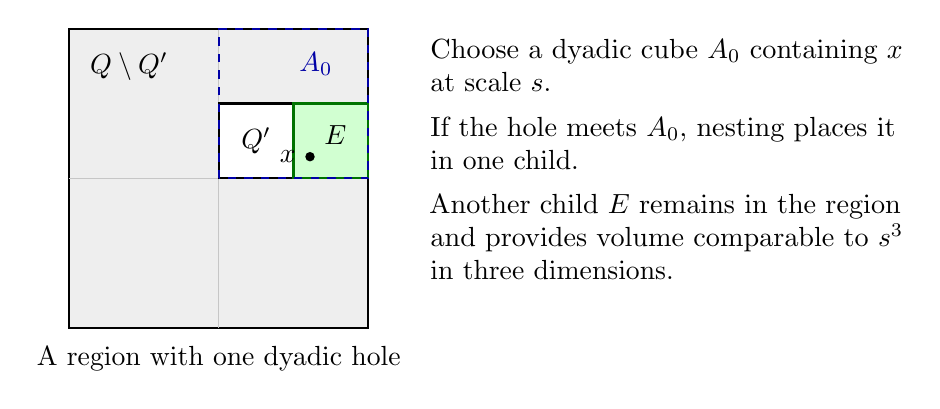
\begin{tikzpicture}[scale=0.95]
 \fill[gray!13] (0,0) rectangle (4,4);
 \draw[thick] (0,0) rectangle (4,4);
 \draw[gray!45] (2,0)--(2,4) (0,2)--(4,2);
 \fill[white] (2,2) rectangle (3,3);
 \draw[thick] (2,2) rectangle (3,3);
 \fill[green!18] (3,2) rectangle (4,3);
 \draw[green!45!black,thick] (3,2) rectangle (4,3);
 \draw[blue!65!black,dashed,thick] (2,2) rectangle (4,4);
 \fill (3.22,2.29) circle (1.8pt);
 \node[anchor=east] at (3.16,2.29) {$x$};
 \node at (2.5,2.5) {$Q'$};
 \node at (3.56,2.58) {$E$};
 \node[blue!65!black] at (3.3,3.53) {$A_0$};
 \node at (0.8,3.5) {$Q\setminus Q'$};
 \node[anchor=north] at (2,-0.12) {A region with one dyadic hole};
 \node[align=left,anchor=west,text width=6.0cm] at (4.7,2.25)
 {Choose a dyadic cube $A_0$ containing $x$ at scale $s$.\\[4pt]
  If the hole meets $A_0$, nesting places it in one child.\\[4pt]
  Another child $E$ remains in the region and provides volume
  comparable to $s^3$ in three dimensions.};
\end{tikzpicture}
\caption{A two-dimensional illustration of the thickness argument in
Lemma~\ref{mot:partition}.  The volume estimate is proved for
three-dimensional cubes.  It holds near the hole as well as near the
outer boundary, and survives every rigid motion.  This makes the
packing argument independent of the depth of the dyadic subdivision.}
\label{mot:partition-figure}
\end{figure}

\FloatBarrier

\subsection{Counting prescribed images of rich lines}

We give the two elementary geometric facts needed for the line-type
contributions.  In the first lemma a line-match weight is the full
number of source points on the specified line mapped to target
points on its specified image line.

\begin{lemma}[Two prescribed line images]
\label{mot:line-images}
Let \((L_1,L_2)\) and \((L'_1,L'_2)\) be ordered pairs of distinct
affine lines in \(\mathbb R^3\).
\begin{enumerate}
\item If the source lines are nonparallel, at most eight rigid
motions map \(L_i\) onto \(L'_i\) for \(i=1,2\).
\item If the source lines are parallel, the target lines must be
parallel at the same positive separation.  There are at most four
possible orthogonal linear parts, and for each one the admissible
translations form one affine line parallel to the target lines.
If all four lines contain at most \(H\) points of their respective
clouds, then
\begin{equation}
\label{mot:parallel-weight}
 \sum_g w_1(g)w_2(g)\le4H^3,
\end{equation}
where only motions with positive product are included.  That set
of motions is finite.
\end{enumerate}
Both conclusions allow both orientation classes.
\end{lemma}

\begin{proof}
For nonparallel lines choose unit directions \(a_1,a_2\) and
\(b_1,b_2\).  The orthogonal part \(S\) of a motion must satisfy
\(Sa_i=\varepsilon_i b_i\), with
\(\varepsilon_i\in\{1,-1\}\).  There are at most four sign
choices.  Each compatible choice determines the isometry on the
two-dimensional span of \(a_1,a_2\), and there are at most two
choices on its perpendicular line.  For each resulting \(S\),
the condition on its translation \(h\) imposed by each line is
an affine line in translation space with direction \(b_i\).
Those two affine lines are nonparallel, so their intersection
has at most one point.  This proves the bound of eight, whether
the original lines intersect or are skew.

For parallel lines choose unit directions \(a,b\).  Let \(d\)
be the nonzero perpendicular separation vector from \(L_1\) to
\(L_2\), and let \(e\) be the analogous vector for the ordered
target pair.  Orthogonality forces
\[
 Sa=\pm b,\qquad Sd=e.
\]
These equations determine \(S\) on a two-dimensional space,
with at most two choices on its perpendicular line.  There are
therefore at most four orthogonal parts in total.  For any fixed
one, mapping the first source line onto the first target line
fixes the translation modulo a scalar multiple of \(b\); the
second-line condition is then either impossible or automatically
satisfied.  This proves the geometric assertion.

Parametrize one such translation family by a real number \(\tau\).
Each pair of a source sample point on \(L_1\) and a target sample
point on \(L'_1\) determines a unique \(\tau\).  Thus
\[
 \sum_\tau w_1(\tau)
 \le |X\cap L_1|\,|Y\cap L'_1|\le H^2,
 \qquad w_2(\tau)\le H.
\]
Only finitely many \(\tau\) have positive first weight.  The
product sum for this linear part is at most \(H^3\); summing over
at most four parts proves \eqref{mot:parallel-weight}.  This
argument sums the actual translations and introduces no
discretization of the continuous family.
\end{proof}

\begin{lemma}[Parallel pairs at a fixed separation]
\label{mot:parallel-pairs}
Let \(\mathcal L\) be a finite family of at most \(L\) distinct
lines in \(\mathbb R^3\).  For each \(\rho>0\), the number of
ordered parallel pairs in \(\mathcal L\) at separation \(\rho\)
is \(O(L^{3/2})\), with an absolute implicit constant.
\end{lemma}

\begin{proof}
In one parallelism class of size \(q\), intersect the lines with
the plane through the origin perpendicular to their common
direction.  Their intersection points are distinct, and line
separation equals the Euclidean distance of these points.
Form the graph whose edges join points at distance \(\rho\).
Two different vertices have at most two common neighbors, because
two distinct circles of radius \(\rho\) have at most two common
points.  If the graph has \(e\) edges and degrees \(d_z\), then
\[
 \sum_z\binom{d_z}{2}\le2\binom q2,
 \qquad
 (2e)^2\le q\sum_zd_z^2\le3q^3.
\]
In the last inequality we used the preceding bound and
\(2e\le q(q-1)\).  Hence there are \(O(q^{3/2})\) ordered
pairs in this class.  Sum over the classes, using
\(\sum_jq_j^{3/2}\le(\sum_jq_j)^{3/2}\le L^{3/2}\).
\end{proof}

\subsection{Proof of the very-rich-motion estimate}

\begin{proof}[Proof of Theorem~\ref{mot:rich}]
We prove the stronger assertion stated at the start of the section.
Let \(X,Y\) be
clouds of at most \(N\) points, put \(A=N^{2/3}\), and suppose
that each line contains at most \(2A\) points of either cloud.
Write \(k_g=k_g(X,Y)\) throughout this proof.  We prove
\eqref{mot:rich-sum} with this notation.  This implies
the asserted result by \eqref{mot:physical-line-cap}.  Alternatively,
the claim for a congruent copy follows by composing the motions
with the inverse of the congruence, which preserves their match
counts and bijects the two orientation classes as appropriate.

Fix the absolute constants
\[
 \alpha=\frac1{14},\qquad
 \beta=\frac1{4K_{\mathrm{part}}},\qquad
 \nu=\frac{\eta_1}{4}.
\]
Choose \(C_{\mathrm{rich}}\) sufficiently large that
\begin{equation}
\label{mot:constant-choices}
 C_{\mathrm{rich}}>4,\qquad
 \frac\beta4 C_{\mathrm{rich}}^{9/14}
      \ge C_{\mathrm{loc}},\qquad
 \eta_1\beta C_{\mathrm{rich}}^{3/7}\ge1,\qquad
 \nu C_{\mathrm{rich}}\ge4.
\end{equation}
All constants on the right have already been fixed.  These choices
are independent of \(N\) and of the clouds.

Every motion with at least \(C_{\mathrm{rich}}A\) matches has a
noncollinear matched triple, because the line cap is \(2A\).
The finite choice of source and target ordered triples and the
at-most-two extensions per triple prove finiteness of the motion
set in the sum.  In particular, possible continuous families of
motions fixing a line are below the threshold unless they have
additional noncollinear matches, in which case this same finite
triple argument applies.

Bucket the high motions by
\[
 k\le k_g(X,Y)<2k,\qquad
 k=tA,\qquad t=2^jC_{\mathrm{rich}}\le N^{1/3}.
\]
If no such \(t\) exists, the sum is empty.  In a nonempty bucket
set
\begin{equation}
\label{mot:subdivision-parameters}
 r=t^{1+\alpha},\qquad
 m=8N/r,\qquad
 b=\beta k/r=\beta A t^{-\alpha}.
\end{equation}
Since \(t\le N^{1/3}\) and \(\alpha<2\), we have
\(1\le r\le N\), so Lemma~\ref{mot:partition} applies to both
clouds.  It supplies at most \(19r\) regions in each partition,
each with at most \(m\) points.

For the partitions just chosen, put \(X_R=X\cap R\) and
\(Y_{R'}=Y\cap R'\).  The local count is
\(n_{R,R'}(g)=k_g(X_R,Y_{R'})\).  These counts sum to \(k_g\),
and at most \(K_{\mathrm{part}}r\) are nonzero.  By
\eqref{mot:region-discard}, discarding those below \(b\) removes
at most \(K_{\mathrm{part}}rb=k/4\) matches.  At least \(3k/4\)
matches remain.
Bucket each remaining local count into
\(\ell\le n_{R,R'}(g)<2\ell\), with \(\ell=2^i b\), and
use the line/planar/general classification of
Lemma~\ref{mot:local} for the clouds \(X_R,Y_{R'}\) in that local
bucket.  A single global motion may contribute different local types
in different region pairs.

The local lower threshold is valid, since
\begin{equation}
\label{mot:local-scale-check}
 \frac{b}{m^{2/3}}
 =\frac\beta4\,t^{(2-\alpha)/3}
 =\frac\beta4\,t^{9/14}
 \ge C_{\mathrm{loc}}.
\end{equation}
We shall also need the full-cloud rich-line threshold
\(q=\eta_1b\) to be at least \(\sqrt N\).  The inequality
\(t\le N^{1/3}\) gives \(N^{1/6}\ge t^{1/2}\), so
\begin{equation}
\label{mot:rich-line-scale}
 \frac{q}{\sqrt N}
 =\eta_1\beta N^{1/6}t^{-\alpha}
 \ge\eta_1\beta t^{1/2-\alpha}
 =\eta_1\beta t^{3/7}\ge1.
\end{equation}
In particular these rich lines contain at least two points in every
nonempty bucket.  One may also record the power margin
\(b\ge\beta N^{9/14}\), although only
\eqref{mot:rich-line-scale} is needed below.

\paragraph{Motions with substantial non-line-type mass.}
Let \(\mathcal G_0\) consist of the motions in the global bucket
whose retained local non-line-type counts have total at least
\(k/4\).  For a fixed region pair and a local richness bucket,
Lemma~\ref{mot:local} bounds the number of non-line-type motions
by \(K_{\mathrm{loc}}m^3/\ell^{3/2}\).  Their local match mass
is therefore at most \(2K_{\mathrm{loc}}m^3/\sqrt\ell\).
Summing the geometric series over \(\ell=2^i b\) gives
\(O(m^3/\sqrt b)\) for each fixed region pair.  The bound remains
valid after restriction to our global bucket.  There are at most
\((19r)^2\) possible region pairs, whence
\begin{equation}
\label{mot:nonline-mass}
 |\mathcal G_0|\,k^2
 \le C k r^2\frac{m^3}{\sqrt b}
 \le C' N^3\frac{k}{r\sqrt b}
 =C''N^3\sqrt A\,t^{-\alpha/2}
 =C''\frac{N^4}{A}\,t^{-1/28}.
\end{equation}
The equality \(N^3\sqrt A=N^4/A\) uses \(A=N^{2/3}\).

\paragraph{Motions whose retained mass is mostly line type.}
For every remaining motion, at least \(k/2\) retained matches
belong to line-type local buckets.  In each such region pair,
choose one source line containing at least \(\eta_1\ell\) of
its local matches, and retain those matches as assigned line
matches.  Since \(n_{R,R'}(g)<2\ell\), this retains at least
\(\eta_1/2\) of that local count.  Thus the assigned line-match
mass \(W_g\) satisfies
\[
 W_g\ge\nu k,\qquad \nu=\eta_1/4.
\]
A physical source point participates in at most one region-pair
count for a fixed motion.  Hence no assigned match is repeated.
Pool assignments belonging to the same full source line \(L\),
and write its weight as \(w_{g,L}\).  Its target line is necessarily
\(gL\), and
\begin{equation}
\label{mot:pooled-line-weights}
 \sum_Lw_{g,L}=W_g\ge\nu k,
 \qquad 0\le w_{g,L}\le2A.
\end{equation}
Every line appearing on either side contains at least
\(\eta_1b=q\) ambient sample points, because it was chosen in a
local bucket with \(\ell\ge b\).

Let \(\mathcal L_X,\mathcal L_Y\) be the full lists of these
\(q\)-rich lines of the two clouds.  These are finite lists of
spanned lines.  Equations~\eqref{mot:st-rich} and
\eqref{mot:rich-line-scale} imply
\begin{equation}
\label{mot:rich-line-number}
 |\mathcal L_X|,|\mathcal L_Y|
 \le C\left(\frac{N^2}{q^3}+\frac Nq\right)
 \le C'\frac Nb.
\end{equation}
Denote a common upper bound in \eqref{mot:rich-line-number} by
\(L_*=C'N/b\).

The diagonal weights can be removed without losing a fixed
fraction.  Indeed, by \eqref{mot:constant-choices} and
\eqref{mot:pooled-line-weights},
\(W_g\ge\nu k\ge4A\).  Consequently
\begin{equation}
\label{mot:distinct-line-pair-mass}
 \sum_{L_1\ne L_2}w_{g,L_1}w_{g,L_2}
 =W_g^2-\sum_Lw_{g,L}^2
 \ge W_g^2-2AW_g
 \ge\tfrac12\nu^2 k^2.
\end{equation}

Sum this quantity over the remaining motions.  For nonparallel
source line pairs, there are at most \(L_*^4\) prescriptions of
an ordered source pair and its ordered target pair.  By
Lemma~\ref{mot:line-images}, each prescription has at most eight
motions, and each product of weights is at most \((2A)^2\).
Their total contribution is thus \(O(A^2L_*^4)\).

For a parallel ordered source pair, fix its positive separation
\(\rho\).  Lemma~\ref{mot:parallel-pairs} gives at most
\(O(L_*^{3/2})\) ordered target pairs at that separation, including
all target parallelism classes.  There are at most \(L_*^2\)
source pairs.  For every prescription, the pooled selected weights
are bounded by the full line-match weights in
Lemma~\ref{mot:line-images}; with \(H=2A\), its bound is
\(O(A^3)\).  Therefore the total parallel contribution is
\(O(A^3L_*^{7/2})\).

If \(\mathcal G_1\) denotes the remaining motions, the two cases
and \eqref{mot:distinct-line-pair-mass} give
\begin{equation}
\label{mot:line-mass}
 |\mathcal G_1|\,k^2
 \le C\left(A^2(N/b)^4+A^3(N/b)^{7/2}\right).
\end{equation}
This counts both orientations.  In the parallel case it sums the
whole continuous translation family through its finite positive
match support, rather than assuming a bounded number of motions
for the two prescribed lines.

\paragraph{Summing the global buckets.}
From \(b=\beta A t^{-\alpha}\), with its fixed positive
\(\beta\), the two terms in \eqref{mot:line-mass} are
\begin{align}
\label{mot:nonparallel-exponent}
 A^2(N/b)^4&=O\left(N^{8/3}t^{4\alpha}\right)
             =O\left(N^{8/3}t^{2/7}\right),\\
\label{mot:parallel-exponent}
 A^3(N/b)^{7/2}&=O\left(N^{19/6}t^{7\alpha/2}\right)
             =O\left(N^{19/6}t^{1/4}\right).
\end{align}
Summing these increasing geometric series up to
\(t\le N^{1/3}\) gives respectively
\[
 O\left(N^{58/21}\right)
 \quad\text{and}\quad
 O\left(N^{13/4}\right).
\]
Both are bounded by \(O(N^{10/3})=O(N^4/A)\); in fact they save
the powers \(N^{-4/7}\) and \(N^{-1/12}\), respectively.
The decreasing geometric series in
\eqref{mot:nonline-mass} gives
\[
 \sum_{j\ge0}
 O\left(\frac{N^4}{A}
       (2^jC_{\mathrm{rich}})^{-1/28}\right)
 =O(N^4/A).
\]
Finally \(k_g<2k\) in each global bucket, so replacing its
cardinality times \(k^2\) by the sum of the actual \(k_g^2\)
costs at most a factor of four.  The two types exhaust every
bucket, proving \eqref{mot:rich-sum}.
\end{proof}

\begin{remark}[Scope of the threshold and the deletion cost]
\label{mot:scope}
The finite line cap is essential for the sum over motions to make
sense.  For a collinear sample without such a high threshold,
infinitely many rotations about its containing line fix every
point.  In Theorem~\ref{mot:rich} each counted motion has a
noncollinear matched triple, which removes this issue.
For the reduction in this paper, \(M=o(A)\) guarantees the finite
hypothesis \(M\le A\) eventually.  Deleting every existing graph
edge whose endpoints are matches of the same motion above the threshold
costs at most \(\sum_g\binom{k_g}{2}=O(N^4/A)\).  Counting an edge for
several motions can only increase this upper bound.  In the proof of
Lemma~\ref{red:local-concentration}, the real Gram-matrix calculation
uses this deletion to bound the parameters in every local maximal
isotropic plane.
\end{remark}

\appendix
\section{Uniform concentration of evaluation flats}
\label{conc:section}

We prove the algebraic estimate used twice in the distance argument.  Its
constant is uniform in the scale parameter.  The distinction between the
two versions below is essential: the global family has a cardinality
bound, whereas a family inside one of its flats need not have one.

Throughout this section, varieties are reduced complex algebraic
varieties.  The degree of an affine variety means the degree of its
projective closure; the degree of a pure-dimensional union is the sum of
the degrees of its irreducible components.  Constants denoted by $C_e$
may change from line to line and depend only on $e$.

Let $E$ be a complex vector space of dimension $e\geq3$, and write
\[
 S=\bigwedge^2E^*,\qquad n=\binom e2,\qquad
 r=e-1,\qquad s_0=n-r=\binom{e-1}{2}.
\]
An element $z\in S$ is regarded as a skew map $E\to E^*$.  Set
\[
 \mathcal Q=\{[v:y]\in\mathbf P(E\oplus E^*):y(v)=0\}.
\]
For $\lambda=[v:y]\in\mathcal Q$ with $v\ne0$, define
\begin{equation}
 F_\lambda=\{z\in S:zv=y\},\qquad
 K_v=\{z\in S:zv=0\}.
 \label{conc:flat-model}
\end{equation}
Evaluation at $v$ maps $S$ onto the $r$-dimensional annihilator of $v$.
Consequently $F_\lambda$ is a nonempty affine $s_0$-flat, with direction
$K_v=\bigwedge^2(E/\mathbb Cv)^*$.  Distinct parameters give distinct
flats.  Indeed, the common radical of the forms in $K_v$ is exactly
$\mathbb Cv$: the quotient has dimension at least two, and each of its
nonzero vectors is detected by an alternating form.  The direction of
the flat therefore recovers $[v]$, and its prescribed evaluation recovers
$y$ with the same normalization.

A maximal projective linear subspace of $\mathcal Q$ is a
$\mathbf P^r$.  Equivalently, it is the projectivization of an
$e$-dimensional totally isotropic subspace for the quadratic form
$(v,y)\mapsto y(v)$.

\begin{theorem}[Uniform concentration]
\label{conc:theorem}
Fix $C_0\geq1$.  Let $A\geq1$ and let $\mathcal P$ be a finite set of
distinct parameters $[v:y]\in\mathcal Q$, all with $v\ne0$.  Assume:
\begin{enumerate}
\item[(i)] For every $\lambda\in\mathcal P$ there is a homogeneous polynomial
      of positive degree at most $C_0A$ which is nonzero at $\lambda$ and
      zero at every other member of $\mathcal P$.
\item[(ii)] Every projective $\mathbf P^r\subset\mathcal Q$ contains at most
      $C_0A^{r-1}$ members of $\mathcal P$.
\end{enumerate}
There is a constant $C=C(e,C_0)$ such that
\begin{equation}
 \#\{\lambda\in\mathcal P:F_\lambda\subset V\}
 \leq C\deg(V)A^h,
 \qquad \dim V=s_0+h,\quad 1\leq h<r,
 \label{conc:bound}
\end{equation}
for irreducible proper affine varieties $V\subset S$, in either of these
settings:
\begin{enumerate}
\item[(a)] All such $V$ are allowed, and $|\mathcal P|\leq C_0A^r$.
\item[(b)] Only $V$ contained in the zero set of some nonzero polynomial
      of degree at most $C_0A$ are allowed.  No bound on
      $|\mathcal P|$ is required.
\end{enumerate}
\end{theorem}

For $h=0$, an irreducible variety containing an $s_0$-flat must equal
that flat, so it contains at most one member of the family.  In (a) the
ambient endpoint $h=r$ is supplied by the cardinality assumption.  As a
useful consequence of (b), a nonzero polynomial of degree $D\leq C_0A$
contains at most $CDA^{r-1}$ of the flats in its zero set: apply
\eqref{conc:bound} to its irreducible hypersurface components and sum
their degrees.

The proof first obtains approximate equations and regular defining
equations (Theorem~\ref{aci:theorem} and Lemma~\ref{conc:regularity}),
then recovers controlled families of actual rulings
(Lemma~\ref{conc:rulings}). Proposition~\ref{conc:degree} bounds their degree
and identifies the maximal-isotropic exception.
Section~\ref{conc:uniform-completion} closes the resulting finite
system of inequalities with constants independent of $A$.

We normalize the number of flats contained in a variety by its degree,
following Walsh's concentration parameters
\cite[Section~1.1, definition of \(\mathcal D_m\)]{walsh2023}.  The controlled-ruling strategy and the
isotropic exception are closely related to the three-dimensional
rigid-motion analysis of Tidor, Yu, and Zakharov
\cite[Sections~5--6]{tidoryuzakharov2026}.  Here the ruling geometry is
that of evaluation flats of alternating forms in arbitrary fixed
dimension; the required degree bound and exceptional-family
classification are proved in full below.

\subsection{Approximate complete intersections}
\label{aci:section}

We prove Walsh's approximate complete-intersection theorem
\cite[Theorem~1.3]{walsh2020}. The partial-degree framework and the
construction of compatible cuts follow
\cite[Definition~2.2 and Lemma~5.3]{walsh2020}.
The comparison of restriction spaces appears in the proof of
\cite[Lemma~3.5]{walsh2020}. Walsh obtains a corresponding prefix
degree estimate for his chosen cuts
\cite[Theorem~5.5]{walsh2020}.
We prove the forms needed here; the component Hilbert bounds in
Lemma~\ref{poly:hilbert} are the only quantitative algebraic input.
In particular, this proof is independent
of Theorem~\ref{conc:theorem}.

\begin{theorem}[Approximate complete intersection]
\label{aci:theorem}
\label{conc:walsh}
For every $n$ there is a constant $C_n$ with the following property.
If $V\subset\mathbb A^n_{\mathbb C}$ is irreducible of codimension
$c>0$, there are nonconstant polynomials $f_1,\ldots,f_c\in I(V)$ such
that $V$ is an irreducible component of $Z(f_1,\ldots,f_c)$ and
\[
 \prod_{i=1}^c\deg f_i\le C_n\deg V.
\]
\end{theorem}

Here and below, a component \emph{containing $V$} means that it contains
the whole irreducible variety $V$.  Set
\[
 I_{\le t}(V)=I(V)\cap\mathbb C[x_1,\ldots,x_n]_{\le t},
 \qquad
 H_V(t)=\dim_{\mathbb C}
 \bigl(\mathbb C[x_1,\ldots,x_n]_{\le t}/I_{\le t}(V)\bigr).
\]
For $1\le i\le c$, define $\delta_i$ to be the smallest integer $t$
such that every irreducible component of $Z(I_{\le t}(V))$ containing
$V$ has codimension at least $i$.  The notation $Z(I_{\le t}(V))$
means the zero set of a basis of this finite-dimensional vector space.
Finite generation of $I(V)$ shows that these integers exist, and their
definition gives
\begin{equation}
 1\le\delta_1\le\cdots\le\delta_c.
 \label{aci:partial-degrees}
\end{equation}
We also put $\delta_0=0$.

\begin{lemma}[Compatible partial cuts]
\label{aci:cuts}
There are $f_i\in I_{\le\delta_i}(V)$, $1\le i\le c$, such that
every component of $Z(f_1,\ldots,f_i)$ containing $V$ has codimension
exactly $i$.

For any such choice, if $0\le j<c$ and
$\delta_j\le m<\delta_{j+1}$, some component $W$ of
$Z(f_1,\ldots,f_j)$ containing $V$ satisfies
\begin{equation}
 I_{\le m}(W)=I_{\le m}(V),\qquad H_W(m)=H_V(m).
 \label{aci:shared-rank}
\end{equation}
When $j=0$, the prefix zero set and its unique component are
$\mathbb A^n$.
\end{lemma}

\begin{proof}
Suppose $f_1,\ldots,f_{i-1}$ have been chosen, and list the finitely
many components $W$ of their zero set which contain $V$.  Each has
codimension $i-1$.  None is contained in $Z(I_{\le\delta_i}(V))$:
otherwise a component of that latter set would contain $W$, hence
contain $V$ and have codimension at most $i-1$, contrary to the
definition of $\delta_i$.  Consequently the members of
$I_{\le\delta_i}(V)$ that vanish on any fixed $W$ form a proper
linear subspace.  Choose $f_i$ outside their finite union.  It cuts
every such $W$ properly.  The principal ideal theorem then gives
codimension exactly $i$ for every new component containing $V$.
This includes $i=1$, when the preceding zero set is the ambient space,
and proves the construction.

For the second assertion, suppose no component $W$ in the indicated
prefix has $I_{\le m}(V)\subset I(W)$.  The same finite-union argument
provides $g\in I_{\le m}(V)$ which vanishes identically on none of
them.  All components of $Z(f_1,\ldots,f_j,g)$ containing $V$ then
have codimension $j+1$.  Since $m\ge\delta_j$, every one of these
equations belongs to $I_{\le m}(V)$.  Thus every component of
$Z(I_{\le m}(V))$ containing $V$ has codimension at least $j+1$.
This contradicts $m<\delta_{j+1}$.  For a component $W$ where the
inclusion does hold, the reverse inclusion follows from $V\subset W$,
giving \eqref{aci:shared-rank}.
\end{proof}

\begin{proof}[Proof of Theorem~\ref{aci:theorem}]
Fix the polynomials from Lemma~\ref{aci:cuts}.  We will prove, for
$0\le s\le c$, that every component $U$ of the first $s$ cuts
containing $V$ satisfies
\begin{equation}
 \deg U\ge\gamma_n^{\,s}\prod_{i=1}^s\delta_i
 \label{aci:prefix-degree}
\end{equation}
for one sufficiently small $0<\gamma_n\le1$ depending only on $n$.
For $s=0$ both sides are $1$.

We record the precise consequence of Lemma~\ref{poly:hilbert} used
here.  There are constants $a_n>0$ and $b_n\ge1$ such that an
irreducible $k$-dimensional variety $X$ satisfies
\begin{equation}
 H_X(m)\le b_n\deg(X)m^k\qquad(m\ge1),
 \label{aci:rank-upper}
\end{equation}
and, if $X$ is a component of a system whose equations have degrees at
most $m$, then
\begin{equation}
 H_X(m)\ge a_n\deg(X)m^k\qquad(m\ge1).
 \label{aci:rank-lower}
\end{equation}
The second assertion is the bound at the equation degree in
\eqref{poly:hilbert-at-L}, applied with $L=m$.  It permits other
components of the system to have larger dimension.  The lower bound
also holds for $X=\mathbb A^n$, after decreasing $a_n$, directly from
$H_{\mathbb A^n}(m)=\binom{m+n}{n}$.

Suppose \eqref{aci:prefix-degree} is known for smaller indices, and
let $U$ be a component at index $s$.  If $\delta_s=1$, the entire
product in \eqref{aci:prefix-degree} is $1$, and $\deg U\ge1$ proves
the claim.  Otherwise set
\[
 m=\delta_s-1,\qquad
 j=\max\{i:0\le i<s,\ \delta_i<\delta_s\}.
\]
Thus
\begin{equation}
 \delta_j\le m<\delta_{j+1}
   =\cdots=\delta_s\le2m.
 \label{aci:block}
\end{equation}
Lemma~\ref{aci:cuts} supplies a component $W$ at index $j$ with
$H_W(m)=H_V(m)$.  Its dimension is $n-j$, and the degrees of its
defining prefix equations are at most $\delta_j\le m$.
The induction hypothesis and \eqref{aci:rank-lower} therefore give
\[
 H_V(m)=H_W(m)
 \ge a_n\gamma_n^{\,j}
       \left(\prod_{i=1}^j\delta_i\right)m^{n-j}.
\]
This formula also applies when $j=0$.  Since $V\subset U$, restriction
from $U$ to $V$ is surjective on polynomial restriction spaces, so
$H_U(m)\ge H_V(m)$.  On the other hand, $\dim U=n-s$ and
\eqref{aci:rank-upper} bounds $H_U(m)$ above.  Combining the bounds,
then using \eqref{aci:block}, yields
\[
 \begin{split}
 \deg U
 &\ge \frac{a_n}{b_n}\gamma_n^{\,j}
       \left(\prod_{i=1}^j\delta_i\right)m^{s-j}\\
 &\ge \frac{a_n}{2^n b_n}\gamma_n^{\,j}
       \prod_{i=1}^s\delta_i.
 \end{split}
\]
Choose $\gamma_n\le\min\{1,a_n/(2^n b_n)\}$.  Since $j<s$, the
last expression is at least the right side of
\eqref{aci:prefix-degree}, completing the induction.  Notice that no
containment relation between $U$ and the chosen $W$ was needed; both
contain $V$.

At $s=c$, every prefix component containing $V$ has the same dimension
as $V$, so $V$ itself is such a component.  Applying
\eqref{aci:prefix-degree} to it gives
\[
 \prod_{i=1}^c\deg f_i
 \le\prod_{i=1}^c\delta_i
 \le\gamma_n^{-c}\deg V
 \le\gamma_n^{-n}\deg V.
\]
This proves the theorem with $C_n=\gamma_n^{-n}$.
\end{proof}

The conclusion concerns an irreducible component.  It does not assert
that the displayed equations generate its radical ideal or have
independent differentials; the next regularity argument supplies the
additional control needed here.


\subsection{Separators and regular equations}

We use the isolated-intersection form of B\'ezout, with local
multiplicities, and the standard local algebra and projective-bundle
facts detailed in the proofs below
\cite{fulton1998,hartshorne1977}.

\begin{lemma}[Counting by separators]
\label{conc:separators}
Under the separator assumption of Theorem~\ref{conc:theorem}, an
irreducible projective variety $Y\subset\mathbf P(E\oplus E^*)$ of
dimension $a$ contains at most
\[
 C_{e,C_0}\deg(Y)A^a
\]
sample parameters.  The variety $Y$ need not be contained in
$\mathcal Q$.
\end{lemma}

\begin{proof}
Induct on $a$.  The assertion for $a=0$ says that a point contains at
most one sample parameter.  Otherwise, if $Y\cap\mathcal P\ne\varnothing$,
choose $\lambda\in Y\cap\mathcal P$ and a separator $q$ for it.  Since
$q(\lambda)\ne0$, the section $Y\cap Z(q)$ is proper, and it contains
all the other counted parameters.  Its components have dimension
$a-1$ and total degree at most $C_0A\deg Y$.  Applying the induction
hypothesis to those components gives
\[
 |Y\cap\mathcal P|
 \leq 1+C_{a-1}C_0\deg(Y)A^a.
\]
The initial $1$ is absorbed because $A\geq1$ and $\deg Y\geq1$.
There are only boundedly many possible dimensions.
\end{proof}

\begin{lemma}[Regular equations of controlled degree]
\label{conc:regularity}
Suppose that an irreducible $V\subset\mathbb A^n_{\mathbb C}$ has
codimension $c>0$ and is a component of $Z(f_1,\ldots,f_c)$, where
\[
 \deg f_i\leq D,\qquad
 \prod_i\deg f_i\leq C_n\deg V,\qquad D\geq1,
\]
with the dimensional constant from Theorem~\ref{conc:walsh}.
There are polynomials $g_1,\ldots,g_c\in I(V)$ of degrees $O_n(D)$
whose differentials are independent at the generic point of $V$.
Moreover, a polynomial $H_0$ of degree $O_n(D)$, nonzero on $V$, can be
chosen so that $V\setminus Z(H_0)$ is smooth and has tangent space
\[
 T_zV=\bigcap_{i=1}^c\ker dg_i(z)
 \qquad(z\in V\setminus Z(H_0)).
\]
\end{lemma}

\begin{proof}
Put $P=I(V)$ and consider the regular local ring
\[
 R=\mathbb C[x_1,\ldots,x_n]_P,\qquad
 \mathfrak m=PR,\qquad K=R/\mathfrak m=\mathbb C(V).
\]
Its dimension is $c$.  Because $V$ is an isolated component of the
common zero set at its generic point, $J=(f_1,\ldots,f_c)R$ is
$\mathfrak m$-primary.  Its generators form a parameter sequence,
which is regular because $R$ is Cohen--Macaulay
\cite[Tags~00OQ, 00NQ, and 02JN]{stacksproject}.
We first bound the length of $R/J$ by a dimensional constant.

Write $k=\dim V$.  A general projective linear projection of
$\overline V$ to $\mathbf P^k$, with center in the hyperplane at
infinity disjoint from $\overline V$, is finite and has degree
$\deg V$.  Finiteness follows because a positive-dimensional projective
fiber would meet its hyperplane lying in the projection center.
Restricting to the affine chart and changing affine coordinates gives
base coordinates $t_1,\ldots,t_k$ and complementary coordinates
$w_1,\ldots,w_c$.  Over $F=\mathbb C(t_1,\ldots,t_k)$, the generic
fiber of $V$ is a closed point of $\mathbb A^c_F$ with residue field
$K$, where $[K:F]=\deg V$.  Localizing $F[w_1,\ldots,w_c]$ at that
point gives the same ring $R$.

After extending $F$ to an algebraic closure, this point splits into
$[K:F]$ points, since the extension is separable.  The sum of their
local intersection multiplicities for the equations $f_i$ is
$[K:F]\operatorname{length}_R(R/J)$.  They are isolated common zeros;
other components of the system do not affect their isolated B\'ezout
bound \cite[Theorem~12.3 and Example~12.3.1]{fulton1998}.
The equations $f_i$ define hypersurfaces in regular local ambient
rings, so these factors are Cohen--Macaulay and the isolated
complete-intersection multiplicity equals the quotient length;
see \cite[Example~12.3.7(ii)--(iii)]{fulton1998} for this identification
and its Cohen--Macaulay hypothesis.  Hence
\begin{equation}
 \operatorname{length}_R(R/J)
 \leq\frac{\prod_i\deg f_i}{\deg V}\leq C_n.
 \label{conc:local-length}
\end{equation}
Choose an integer $L=O_n(1)$ at least this length.  The maximal ideal
of an Artinian local ring of length at most $L$ has $L$th power zero,
so
\begin{equation}
 \mathfrak m^L\subset J.
 \label{conc:adic-bound}
\end{equation}

We construct the $g_i$ one at a time.  Suppose $g_1,\ldots,g_u$ have
independent classes in $\mathfrak m/\mathfrak m^2$, where $u<c$.
They are part of a regular parameter system, and therefore
\[
 R_u=R/(g_1,\ldots,g_u),\qquad
 \mathfrak m_u=\mathfrak mR_u
\]
is a regular local ring of positive dimension.  The images of the
$f_i$ generate an ideal containing $\mathfrak m_u^L$.  At least one
image has finite $\mathfrak m_u$-adic order $b$ with $1\leq b\leq L$.
Otherwise all the images would lie in $\mathfrak m_u^{L+1}$, whence
$\mathfrak m_u^L=\mathfrak m_u^{L+1}$ and Nakayama's lemma would give
$\mathfrak m_u^L=0$, impossible in this positive-dimensional regular
local ring.

We need derivatives which do not disturb the already chosen equations.
For $u=0$ use coordinate derivations.  For $u>0$, choose a $u$-square
Jacobian block $J_0$ of $(g_1,\ldots,g_u)$ whose determinant $\Delta$
is nonzero in $K$.  If $J_t$ is any remaining column, form a polynomial
vector field having coefficient $\Delta$ in coordinate $t$ and
coefficients $-\operatorname{adj}(J_0)J_t$ in the chosen coordinates.
These $n-u$ fields, denoted by $\delta_\alpha$, satisfy
\[
 \delta_\alpha g_i=0\quad(1\leq i\leq u)
\]
as polynomial identities.  Thus they extend to $R$ and descend to
$R_u$.  If the $g_i$ have maximum degree $E_u$, the coefficient degrees
of these fields are $O_n(E_u)$.

At the generic point, the fields span the common kernel of the
$d g_i$.  The conormal map
$\mathfrak m/\mathfrak m^2\to K^n$, $f\mapsto df$, is injective there,
as $V$ is generically smooth in characteristic zero.  It follows that
the residue evaluations of the $\delta_\alpha$ span the dual of
$\mathfrak m_u/\mathfrak m_u^2$.  These residue evaluations are
$K$-linear: the extra Leibniz term from differentiating a coefficient
has a factor in $\mathfrak m_u$.

Take an $f_i$ of order $b$ as above.  A derivation lowers adic order by
at most one, so fewer than $b$ of these derivations still give zero
residue.  Some composition of $b$ of them has nonzero residue.  Indeed,
the leading term of $f_i$ belongs to the degree-$b$ piece of the graded
ring of $R_u$ \cite[Tag~00NO]{stacksproject}, namely
\[
 \mathfrak m_u^b/\mathfrak m_u^{b+1}
 \simeq\operatorname{Sym}^b_K(\mathfrak m_u/\mathfrak m_u^2).
\]
Its polarization is nonzero in characteristic zero.  Since the residue
functionals span the dual, some $b$-tuple detects it.  In computing
that residue, terms in which a derivation hits a coefficient retain a
positive-order factor and vanish.  This gives exactly the asserted
iterated derivative.

Stop immediately before the last differentiation and call the resulting
polynomial $g_{u+1}$.  Its residue in $R_u$ is zero, so it belongs to
$P$.  Its derivative has nonzero residue, so its class in
$\mathfrak m_u/\mathfrak m_u^2$ is nonzero.  It adds an independent
conormal.  This procedure uses at most $L-1$ derivatives per stage and
at most $c$ stages.  Applying a polynomial field of coefficient degree
$T$ to a degree-$B$ polynomial gives degree at most $B+T-1$; the bounds
on $L$ and $c$ therefore keep every $g_i$ of degree $O_n(D)$.

Finally choose a $c$-square minor $H_0$ of the Jacobian of the $g_i$
which is nonzero on $V$.  Its degree is $O_n(D)$.  Where it is nonzero,
the common zero set of the $g_i$ is locally smooth of dimension $n-c$.
The contained variety $V$ has the same dimension, so its germ equals
that smooth germ.  This proves the assertion about tangent spaces.
\end{proof}

\subsection{Recovering actual rulings from tangent directions}

In a chart $v_a=1$, a \emph{ruling incidence} is an irreducible set of
pairs $(z,v)$ for which $z+K_v\subset V$.  Its parameter map is
\begin{equation}
 (z,v)\longmapsto[v:zv].
 \label{conc:parameter-map}
\end{equation}
The point of the next lemma is that both the number of such incidences
and the degree of their exceptional set can be controlled.

\begin{lemma}[Controlled ruling incidences]
\label{conc:rulings}
Let $V\subset S$ be irreducible of dimension $k=s_0+h$, with
$1\leq h<r$.  Suppose that $V$ has $c=n-k$ approximate equations as
in Lemma~\ref{conc:regularity}, of maximum degree at most $D$.
There is a polynomial $H$, nonzero on $V$ and of degree $O_e(D)$,
such that, on $\Omega=V\setminus Z(H)$, the following hold.
\begin{enumerate}
\item There are $O_e(1)$ smooth irreducible ruling incidences $\Gamma$.
      Each is closed in $\Omega\times\{v_a=1\}$ for some $a$ and maps
      smoothly and dominantly to $\Omega$.
\item The fibers over $\Omega$ are either finite of bounded size or
      affine lines of normalized vectors $v$.  Denote the fiber
      dimension by $j=0$ or $j=1$.  The latter is possible only if
      $c=1$.
\item Every flat $F_\lambda\subset V$ meeting $\Omega$ is represented
      by at least one incidence.  All other contained flats lie in
      $V\cap Z(H)$.
\item If $\Lambda$ is the projective closure of the parameter image
      of one incidence, then $\dim\Lambda=h+j$.  Every nonempty
      parameter fiber is exactly $F_\lambda\cap\Omega$ and has
      dimension $s_0$.
\end{enumerate}
\end{lemma}

\begin{proof}
Use Lemma~\ref{conc:regularity} to choose $g_1,\ldots,g_c$ and an
initial smooth open set in $V$.  In the construction below we remove
zeros of a bounded number of polynomials, each of degree $O_e(D)$ and
nonzero on $V$.  Their product, together with the initial Jacobian
minor, will be $H$.  We continue to call the current open set $\Omega$.

First consider tangent directions.  Under $S^*=\bigwedge^2E$, the
annihilator of $K_v$ is $v\wedge E$.  A bivector belongs to this space
if and only if its wedge with $v$ is zero.  Thus the necessary
condition $K_v\subset T_zV$ is the linear system
\begin{equation}
 v\wedge dg_i(z)=0\qquad(1\leq i\leq c).
 \label{conc:tangent-equations}
\end{equation}
Its vector solution space has dimension at most two.  To see this,
let a nonzero bivector $w$ satisfy $v\wedge w=0$ for a nonzero $v$.
Splitting off $\mathbb Cv$ shows that $w=v\wedge a$ for some $a$;
the vectors $v'$ satisfying $v'\wedge w=0$ are precisely
$\operatorname{span}(v,a)$.  If two independent conormals had a common
two-dimensional solution space, both would lie in its one-dimensional
exterior square, a contradiction.  A two-dimensional solution space
therefore forces $c=1$.

Work separately in each of the $e$ normalized charts $v_a=1$.
Gaussian elimination over $\mathbb C(V)$, followed by removal of
nonzero rank minors, puts the system throughout $\Omega$ into one of
three forms: no solution, a graph $v=b(z)$, or
\begin{equation}
 v=b(z)+\tau a_1(z).
 \label{conc:direction-graph}
\end{equation}
In the last case choose a free coordinate of $v$ as $\tau$, so that
its coordinate in $b$ is zero and in $a_1$ is one.  All coefficients
are regular on $\Omega$ and admit ambient rational representatives
with numerator and denominator degrees $O_e(D)$, since the matrices
have bounded size.  Rank conditions which vanish generically vanish
on all of $V$; excluding the nonzero minors consequently controls all
remaining fibers.  Denote the resulting solution variety by $\Gamma_0$.
It is a smooth graph over $\Omega$, or a smooth graph over
$\Omega\times\mathbb A^1$.

We now test whether the tangent directions integrate to a contained
flat.  Write $\varepsilon_1,\ldots,\varepsilon_e$ for a basis of $E^*$.
In the chart $v_a=1$, exterior products of the covectors
$\varepsilon_i-v_i\varepsilon_a$, $i\ne a$, form a basis
$B_1(v),\ldots,B_{s_0}(v)$ of $K_v$.  Their coefficients have degree
at most two in $v$.  Consider the horizontal fields
\[
 X_\alpha(z,v)=(B_\alpha(v),0).
\]
Their $z$-components are tangent to $V$, by
\eqref{conc:tangent-equations}.  They are tangent to $\Gamma_0$ if and
only if the derivatives of all coordinates of its graph formula
vanish in direction $B_\alpha(v)$, with $\tau$ fixed in
\eqref{conc:direction-graph}.  Holding $\tau$ fixed is required
because it is one of the coordinates of the normalized vector $v$.
Call these derivative expressions $T_\beta$.

With no free coordinate the $T_\beta$ are rational functions of $z$.
With a free coordinate they are polynomials in $\tau$ of bounded
degree, whose coefficients have ambient rational degree $O_e(D)$.
This follows by substituting \eqref{conc:direction-graph} in the
quadratic expressions $B_\alpha$ and differentiating its rational
coefficients.  Differentiation along $T_zV$ is independent of the
ambient representatives chosen, since it annihilates functions
vanishing on $V$.

Every contained flat passes this first test: on a small open part of
the flat, $v$ is fixed and the direction equations continue to hold.
If every $T_\beta$ is identically zero, retain $\Gamma_0$; its
horizontal fields are already tangent everywhere.  If there is no
free coordinate but one test is nonzero, remove the zero set of its
numerator and discard this chart.  No contained flat in that chart
can meet the remaining open set.

It remains to treat a free coordinate and a nonidentically zero test.
Let $P(\tau)$ be the monic gcd of the tests over $\mathbb C(V)$, and
let $G(\tau)$ be its monic squarefree part.  The Euclidean algorithm
gives identities
\[
 T_\beta=P Q_\beta,\qquad
 P=\sum_\beta U_\beta T_\beta,
 \qquad G\mid P,\quad P\mid G^q
\]
for a bounded integer $q$.  Exclude the poles of all coefficients
used in these identities.  They then show in every remaining fiber
that the common roots of the tests are exactly the roots of $G$.
If $G=1$, the chart contributes nothing.  Otherwise exclude also the
zero set of its discriminant.  The root variety
\[
 \Sigma_G=\{(z,\tau)\in\Omega\times\mathbb A^1:G(z,\tau)=0\}
\]
is now finite \emph{\'etale} over $\Omega$, with bounded degree.  In
particular it is smooth, and its roots form local holomorphic sheets.

All these exclusions have total degree $O_e(D)$.  Indeed, the number
of tests and their degrees in $\tau$ are bounded.  Gcd, squarefree
part, quotient, and discriminant computations therefore use a bounded
number of field operations.  A bounded number of operations on
ambient fractions of degree $O_e(D)$ preserves that degree bound.
Every excluded denominator or pivot has nonzero restriction to $V$.
The same observation applies to the following second test.

Along a contained flat, $G(z,\tau)=0$ persists with $\tau$ fixed.
Thus a second necessary condition is
\[
 R_\alpha(z,\tau)
 =\sum_{m=1}^{n}(B_\alpha(v(z,\tau)))_m
                  \frac{\partial G}{\partial z_m}(z,\tau)=0.
\]
These expressions again have bounded degree in $\tau$ and coefficient
degrees $O_e(D)$.  Form the monic polynomial
\[
 P_2=\gcd(G,R_1,\ldots,R_{s_0})
\]
and exclude the poles needed to specialize its quotient and B\'ezout
identities.  Its root variety $\Sigma_{P_2}$ is empty or finite
\emph{\'etale} over $\Omega$.  Because $G$ remains squarefree and
$P_2$ divides it, the factorization $G=P_2(G/P_2)$ has disjoint root
sets in every remaining fiber.  Thus $\Sigma_{P_2}$ is locally a union
of whole sheets of $\Sigma_G$.

At a point of $\Sigma_{P_2}$, the first test makes $X_\alpha$ tangent
to $\Gamma_0$, where its coordinates are $(B_\alpha(v),0)$ in
$(z,\tau)$.  The second test makes it tangent to $G=0$.  Hence it is
tangent to the selected sheet of $\Sigma_{P_2}$.  No further
sequence of tangency tests is needed.  Retain its irreducible
components as the incidences.  A smooth variety has disjoint
irreducible components.  Each component of this finite \emph{\'etale}
cover maps openly and closedly to the irreducible base, hence
surjectively; their number and fiber sizes are bounded by $\deg G$.

We verify containment rather than merely tangency.  On every retained
incidence the fields $X_\alpha$ are tangent.  Their ambient flows are
\[
 (z,v)\longmapsto(z+tB_\alpha(v),v),
\]
since $v$ is constant.  Uniqueness of local holomorphic flows keeps
these translations in the incidence for small $t$.  Composing them
produces an analytic open subset of $z+K_v$, because the $B_\alpha(v)$
form a basis of $K_v$.  Every polynomial vanishing on $V$ vanishes on
that open subset, hence on the whole affine flat.  Thus every retained
point really represents a contained flat.

After processing all normalized charts, intersect their open sets and
restrict their incidences to this common $\Omega$.  The product of
the excluded polynomials is nonzero on irreducible $V$ and has degree
$O_e(D)$.  Every nonempty restricted incidence remains irreducible and
dominant.  Its fibers are finite of bounded size, except for the
retained affine-line graphs; the latter arose only in codimension one.

If a contained flat meets $\Omega$, choose a chart for its $v$ and a
point of $F_\lambda\cap\Omega$.  Both tests are necessary along that
flat, and the specialized gcd identities therefore place the point in
a retained incidence.  This proves coverage.

Finally fix one incidence and a nonempty fiber of
\eqref{conc:parameter-map}.  Its normalized vector $v$ is fixed, and
the fiber is closed in $F_\lambda\cap\Omega$.  The preceding flows
preserve both $v$ and $zv$ and give an analytic open subset of that
flat in the fiber.  Such an open subset is Zariski dense in the
irreducible variety $F_\lambda\cap\Omega$, so the fiber equals this
whole intersection.  It has dimension $s_0$.  The fiber-dimension
theorem now gives
\[
 \dim\Lambda=\dim\Gamma-s_0=(k+j)-s_0=h+j.
\]
\end{proof}

\subsection{Degree bounds and exceptional parameter families}
\label{conc:deg-section}

The ruling construction bounds the number of incidences and the degree
of the set removed from \(V\). For an incidence with \(j=0\), its
projective parameter closure \(\Lambda\) has dimension \(h\), so
Lemma~\ref{conc:separators} counts at
most \(C\deg(\Lambda)A^h\) sample parameters. A bound
\(\deg\Lambda\le C_e\deg V\) would therefore give the scale required
by Theorem~\ref{conc:theorem}. When \(j=1\), the parameter variety has
dimension \(h+1\), and the separator bound alone would cost one extra
factor of \(A\). The next proposition proves that this case has
\(h=r-1\) and that the parameter variety is a maximal isotropic
\(\mathbf P^r\subset\mathcal Q\), where assumption (ii) gives the
required \(O(A^{r-1})\) bound. The projective incidence bundle
constructed below gives the degree estimate and the tangent constraint
used to classify this exceptional case.

\begin{proposition}
\label{conc:degree}
Let \(V\subsetneq S\) be irreducible of dimension \(k=s_0+h\), where
\(1\le h<r\), and let \(\Gamma\) be a ruling incidence provided by
Lemma~\ref{conc:rulings}.  Write \(j\in\{0,1\}\) for the dimension
of its fibers over the working open subset \(\Omega\subset V\).
Let \(\Lambda\) be the projective closure of its parameter image
\[
 (z,v)\longmapsto[v:zv]
 \quad\hbox{in}\quad
 \mathcal Q=\{[v:y]\in\mathbf{P}(E\oplus E^*):y(v)=0\}.
\]
Then
\[
 \dim\Lambda=h+j,
 \qquad \deg\Lambda\le C_e\deg V.
\]
If \(j=1\), then \(h=r-1\) and \(\Lambda\) is a linear
\(\mathbf{P}^r\subset\mathcal Q\), hence a maximal isotropic
projective subspace.
\end{proposition}

\begin{proof}
The fibers of the parameter map are the nonempty sets
\(F_\lambda\cap\Omega\), of dimension \(s_0\), whereas
\(\dim\Gamma=k+j\).  The fiber dimension theorem therefore gives
\(\dim\Lambda=h+j\).  We prove the degree estimate and the
assertion for \(j=1\) in turn.

\paragraph{Compactifying the parameter space.}
On \(\mathbf{P}(E)\), let \(L=\mathcal O_{\mathbf{P}(E)}(-1)\)
be the tautological line bundle and put
\(Q=(E\otimes\mathcal O)/L\).  Evaluation of a skew form on
the line \(L\) gives the exact sequence
\begin{equation}
 0\longrightarrow K\longrightarrow S\otimes\mathcal O
 \longrightarrow Q^*\otimes L^*\longrightarrow0,
 \qquad K=\bigwedge^2 Q^*.
 \label{conc:deg-evaluation}
\end{equation}
Indeed, the value of a skew form on \(L\) is a map from \(L\)
to its annihilator \(L^\perp\subset E^*\), every such map
extends to a skew form on \(E\), and the kernel consists of the
forms on \(E/L\).  The ranks of these three bundles are
\(s_0,n,r\), respectively.

All projective bundles below parametrize lines.  Consider
\begin{equation}
 B=\mathbf{P}\bigl(\mathcal O\oplus Q^*\otimes L^*\bigr)
   \simeq\mathbf{P}(L\oplus Q^*),
 \qquad \rho:B\longrightarrow\mathbf{P}(E).
 \label{conc:deg-parameter-bundle}
\end{equation}
The second presentation is obtained by tensoring the first bundle
with \(L\).  We use the line convention of
\cite[Section~3.1 and Example~3.1.1]{fulton1998}.  Since \(L\oplus Q^*\)
is a subbundle of the trivial bundle with fiber \(E\oplus E^*\),
it induces a morphism \(\mu:B\to\mathcal Q\).  Explicitly,
write a point in the first presentation as \((L,[t:\psi])\),
with \(\psi:L\to L^\perp\).  For any nonzero \(v\in L\),
\begin{equation}
 \mu(L,[t:\psi])=[tv:\psi(v)].
 \label{conc:deg-parameter-map}
\end{equation}
Both rescaling \((t,\psi)\) and replacing \(v\) by another
generator of \(L\) leave this point unchanged.  Its quadratic
value is zero because \(\psi(v)\) annihilates \(v\).

Over \(\mathcal Q^\circ=\{[v:y]\in\mathcal Q:v\ne0\}\),
the inverse to \(\mu\) recovers \(L=\mathbb{C}v\) and
\([1:\psi]\), where \(\psi(v)=y\).  Thus \(\mu\) is an
isomorphism over this open set.  A boundary point \([0:y]\)
has fiber \(\mathbf{P}(\ker y)\): its preimages have \(t=0\),
and \(L\) can be any line annihilated by \(y\).

Let \(\mathcal T=\mathcal O_B(-1)\) be the tautological line
in the \emph{first} presentation of
\eqref{conc:deg-parameter-bundle}, and set
\[
 a=\rho^*c_1\bigl(\mathcal O_{\mathbf{P}(E)}(1)\bigr),
 \qquad b=c_1(\mathcal T^*),
 \qquad \ell=\mu^*c_1\bigl(\mathcal O_{\mathcal Q}(1)\bigr).
\]
The tautological line in the second presentation is
\(\mathcal T\otimes\rho^*L\).  Consequently
\begin{equation}
 \ell=a+b.
 \label{conc:deg-hyperplane}
\end{equation}
The classes \(a\) and \(\ell\) are globally generated.  We do
not need positivity of \(b\).

\paragraph{The projective incidence and its boundary.}
Pull back \eqref{conc:deg-evaluation} to \(B\).  Define
\(\mathcal U\) as the inverse image of \(\mathcal T\)
under the surjective bundle map
\[
 (\mathbb{C}\oplus S)\otimes\mathcal O_B
 \longrightarrow
 \mathcal O_B\oplus\rho^*(Q^*\otimes L^*),
 \qquad (x_0,z)\longmapsto(x_0,z|_L).
\]
It is a vector bundle of rank \(s_0+1\), with exact sequence
\begin{equation}
 0\longrightarrow\rho^*K\longrightarrow\mathcal U
 \longrightarrow\mathcal T\longrightarrow0.
 \label{conc:deg-incidence-bundle}
\end{equation}
Its inclusion in the trivial bundle defines a morphism
\(\mathbf{P}(\mathcal U)\to\mathbf{P}(\mathbb{C}\oplus S)\).
The pullback of the hyperplane class under this morphism is
\[
 \xi=c_1\bigl(\mathcal O_{\mathbf{P}(\mathcal U)}(1)\bigr).
\]
For a parameter represented by \((L,[1:\psi])\), choose
\(v\in L\setminus\{0\}\) and write \(y=\psi(v)\).
The projective fiber maps isomorphically to
\begin{equation}
 \{[x_0:z]:zv=x_0y\}=\overline{F_{[v:y]}}.
 \label{conc:deg-flat-closure}
\end{equation}
Over \((L,[t:\psi])\), the defining condition is instead
\((x_0,z|_L)\in\mathbb{C}(t,\psi)\).  In particular,
\begin{equation}
 t=0\quad\Longrightarrow\quad x_0=0.
 \label{conc:deg-boundary}
\end{equation}
Thus no boundary parameter occurs over an affine point \([1:z]\).

Lift the parameter image of \(\Gamma\) to \(B\) using the
isomorphism over \(\mathcal Q^\circ\), and denote its reduced
irreducible closure by \(\widetilde\Lambda\).  The map
\(\mu:\widetilde\Lambda\to\Lambda\) is birational.  Put
\[
 X=\mathbf{P}(\mathcal U|_{\widetilde\Lambda}),
 \qquad \pi:X\longrightarrow\widetilde\Lambda.
\]
The variety \(X\) is irreducible and has dimension
\(s_0+h+j=k+j\).  The point coordinate and the lifted parameter
give an embedding of \(\Gamma\) as a locally closed subset of
\(X\): in its normalized direction chart the inverse recovers
the original pair \((z,v)\).  Since the dimensions agree, this
subset is dense and contains a dense open subset of \(X\).
The projective point map on \(X\) therefore has image exactly
\(\overline V\).  More explicitly, its image is closed by
properness; density shows that it is contained in the closure of
the point image of \(\Gamma\), and dominance of
\(\Gamma\to\Omega\) gives the opposite inclusion.  We obtain
a surjective morphism
\[
 f:X\longrightarrow\overline V,
 \qquad
 \xi=f^*c_1\bigl(\mathcal O_{\overline V}(1)\bigr).
\]
Here and below we also use \(a,b,\ell\) for their restrictions
and pullbacks to the varieties on which they occur.

\paragraph{The degree of a generic point fiber.}
Fix an affine \(z\in S\).  By \eqref{conc:deg-boundary}, the
full incidence over \([1:z]\), before restriction to
\(\widetilde\Lambda\), has parameters \([v:zv]\) with
\(v\ne0\), and is isomorphic to \(\mathbf{P}(E)\).
On this projective space \(\ell\) is the ordinary hyperplane
class: the map \([v]\mapsto[v:zv]\) is induced by an injective
linear map \(E\to E\oplus E^*\).

Choose a dense open subset \(X^\circ\subset X\) lying in the
lift of \(\Gamma\).  Every component of its complement has
dimension at most \(k+j-1\).  A component which dominates
\(V\) therefore has generic fiber dimension at most \(j-1\);
a component which does not dominate \(V\) is absent over a
general point.  The complement cannot supply a top-dimensional
component of the generic fiber of \(f\).

When \(j=0\), the generic fiber thus consists of at most \(C_e\)
points, as does the fiber of \(\Gamma\to\Omega\).  When
\(j=1\), the generic fiber of \(\Gamma\to\Omega\) is an
affine line of normalized vectors.  Its closure in \(\mathbf{P}(E)\)
is a projective line, of degree one against \(\ell\), and this
is the only top-dimensional generic fiber component of \(f\).
These components have multiplicity one.  Indeed, the fibers on
the dense open ruling incidence are smooth: its projection is
finite \'etale or a smooth affine-line family.  This determines
the generic multiplicity of each component, which cannot be
changed by a complement of smaller fiber dimension.

If \(d_\Gamma\) denotes the degree of the geometric generic
fiber against \(\ell^j\), we have proved
\begin{equation}
 d_\Gamma\le C_e,
 \qquad d_\Gamma=1\quad\hbox{when }j=1.
 \label{conc:deg-fiber-degree}
\end{equation}
Proper pushforward and the projection formula, applied to
fundamental cycles, now give
\begin{equation}
 f_*(\ell^j\cap[X])=d_\Gamma[\overline V],
 \qquad
 \int_X\ell^j\xi^k=d_\Gamma\deg V\le C_e\deg V.
 \label{conc:deg-point-integral}
\end{equation}
The coefficient in the first identity is computed on the generic
fiber.  Any other component of a representative hyperplane
intersection has image of dimension less than \(k\) and pushes
forward to zero.  These formulas do not require smoothness of
\(X\) or \(\overline V\); see
\cite[Sections 1.4, 2.3, 2.5]{fulton1998}.

\paragraph{A positive Segre-class formula.}
For projective bundles of lines, the projective bundle formula is
\begin{equation}
 \pi_*(\xi^{s_0+h}\cap[X])
   =s_h(\mathcal U|_{\widetilde\Lambda})
      \cap[\widetilde\Lambda],
 \qquad s_t(\mathcal U)=c_t(\mathcal U)^{-1}.
 \label{conc:deg-projective-bundle}
\end{equation}
This formula applies equally to a vector bundle on a singular
base \cite[Sections 3.1--3.3]{fulton1998}.  We compute it before
restriction to \(\widetilde\Lambda\).

Dualizing the tautological sequence on \(\mathbf{P}(E)\) and
tensoring by \(L^*=\mathcal O(1)\) gives
\[
 0\longrightarrow Q^*(1)
 \longrightarrow E^*\otimes\mathcal O(1)
 \longrightarrow\mathcal O(2)\longrightarrow0.
\]
Together with \eqref{conc:deg-evaluation}, this implies
\[
 c_t(K)^{-1}=c_t(Q^*(1))=\frac{(1+at)^e}{1+2at}.
\]
Since \(c_t(\mathcal T)=1-bt\), Equations
\eqref{conc:deg-incidence-bundle} and
\eqref{conc:deg-hyperplane} yield
\begin{equation}
 s_t(\mathcal U)
   =\frac{(1+at)^e}{(1+2at)(1-bt)}
   =\frac{(1+at)^e}{(1+2at)(1+(a-\ell)t)}.
 \label{conc:deg-segre-series}
\end{equation}
Expanding
\[
 \frac{1}{1+(a-\ell)t}
   =\sum_{i\ge0}\frac{\ell^i t^i}{(1+at)^{i+1}}
\]
and taking the coefficient of \(t^h\) gives
\begin{equation}
 s_h(\mathcal U)
 =\sum_{i=0}^h \ell^i a^{h-i}c(e-1-i,h-i),
 \qquad
 c(p,u)=[z^u]\frac{(1+z)^p}{1+2z}.
 \label{conc:deg-segre-coefficients}
\end{equation}

For integers \(p\ge u+1\) and \(u\ge0\), these scalar
coefficients are nonnegative.  Indeed,
\(c(p,0)=1\), and \(c(p,1)=p-2\ge0\) in its asserted
range.  For \(u\ge2\), the identity
\((1+z)^2=(1+2z)+z^2\) gives
\[
 c(p,u)=\binom{p-2}{u}+c(p-2,u-2).
\]
The second term lies in the same range, because
\(p-2\ge(u-2)+1\).  Induction proves the claim, with a
binomial coefficient equal to zero when its lower index exceeds
its upper index.  In \eqref{conc:deg-segre-coefficients}, the
required inequality is
\(e-1-i\ge h-i+1\), which follows from
\(h\le r-1=e-2\).  The coefficient of \(\ell^h\) is
\(c(e-1-h,0)=1\).

All mixed top intersections of \(a\) and \(\ell\) on
\(\widetilde\Lambda\) are nonnegative.  They can be computed
by successive general members of globally generated linear
systems, whose intersections with the fundamental cycle are
effective or empty.  Birationality of
\(\widetilde\Lambda\to\Lambda\), followed by
\eqref{conc:deg-segre-coefficients},
\eqref{conc:deg-projective-bundle}, and
\eqref{conc:deg-point-integral}, therefore gives
\begin{equation}
 \deg\Lambda
 =\int_{\widetilde\Lambda}\ell^{h+j}
 \le\int_{\widetilde\Lambda}\ell^j s_h(\mathcal U)
 =\int_X\ell^j\xi^k
 \le C_e\deg V.
 \label{conc:deg-bound}
\end{equation}

\paragraph{The tangent constraint in the affine-line case.}
Suppose now that \(j=1\).  Lemma~\ref{conc:rulings} gives
\(\operatorname{codim}_S V=1\), so \(h=r-1\) and
\(\dim\Lambda=r\).  We first show that the tangent space of
\(\Lambda\) at a general smooth point is maximal isotropic for
the tangent quadratic form of \(\mathcal Q\).

Choose a general smooth parameter \(\lambda=[v:y]\in
\Lambda\cap\mathcal Q^\circ\), fix \(z_0\in F_\lambda\),
and let \(U=E/\mathbb{C}v\), of dimension \(r\).  With a
representative \((v,y)\) fixed, tangent vectors to \(\mathcal Q\)
are pairs \((\dot v,\dot y)\) satisfying
\(\dot y(v)+y(\dot v)=0\), modulo \(\mathbb{C}(v,y)\).
There is an isomorphism
\begin{equation}
 T_\lambda\mathcal Q\longrightarrow U\oplus U^*,
 \qquad
 (\dot v,\dot y)\longmapsto
 (\alpha,\beta)=(\dot v\bmod v,\dot y-z_0\dot v).
 \label{conc:deg-tangent-coordinates}
\end{equation}
The covector \(\beta\) annihilates \(v\), by skew symmetry
and \(z_0v=y\).  Adding a multiple of \((v,y)\) changes
neither coordinate, and the kernel before quotienting is exactly
that line, proving the isomorphism.  The tangent quadratic form,
defined up to scale on \(\lambda^\perp/\lambda\), becomes
\(\beta(\alpha)\), because
\[
 (\dot y-z_0\dot v)(\dot v)=\dot y(\dot v).
\]
Let \(\Theta\subset U\oplus U^*\) be the resulting
\(r\)-dimensional image of \(T_\lambda\Lambda\).

The affine incidence over the smooth part of
\(\Lambda\cap\mathcal Q^\circ\) is an affine bundle with
fibers \(F_\lambda\), and its point image lies in \(V\) by
the preceding compactification.  At a point
\(z=z_0+D\in F_\lambda\), with
\(D\in K_v=\bigwedge^2U^*\), differentiating \(zv=y\)
gives
\[
 \dot z\,v=\dot y-z\dot v=\beta-D\alpha.
\]
The vertical tangent space maps onto \(K_v\).  Evaluation at
\(v\) identifies \(S/K_v\) with \(U^*\), so modulo these
vertical directions the differential is
\begin{equation}
 \Theta\longrightarrow U^*,
 \qquad (\alpha,\beta)\longmapsto\beta-D\alpha.
 \label{conc:deg-skew-pencil}
\end{equation}
Every parameter tangent vector lifts because the incidence is an
affine bundle.  At general points its differential has rank at
most \(\dim V=n-1\).  Hence \eqref{conc:deg-skew-pencil}
has rank less than \(r\) for general \(D\) and general
\(\lambda\).  Its determinant is polynomial in the entries of
\(D\); for each general \(\lambda\) it therefore vanishes
for every skew form \(D\) on \(U\).

\paragraph{Linear algebra of the singular skew pencil.}
We prove that this determinant condition forces \(\Theta\)
to be isotropic.  Put
\[
 B_*=\Theta\cap U^*,\qquad
 A_*=\operatorname{pr}_U(\Theta),\qquad
 H_*=B_*^\perp\subset U.
\]
If \(p=\dim A_*\), then \(\dim B_*=r-p\) and
\(\dim H_*=p\).  The plane \(\Theta\) defines a linear map
\[
 C:A_*\longrightarrow U^*/B_*\simeq H_*^*.
\]
The map in \eqref{conc:deg-skew-pencil} is the identity on
\(B_*\).  On taking the quotient by this subspace, the
determinant condition is precisely
\begin{equation}
 \det\bigl(C-D|_{A_*\times H_*}\bigr)=0
 \qquad\hbox{for every }D\in\bigwedge^2U^*.
 \label{conc:deg-quotient-pencil}
\end{equation}
Here the restriction is regarded as a map \(A_*\to H_*^*\).
If \(p=0\), the original map is the identity on \(U^*\),
a contradiction.  Thus \(p>0\).

We claim that \(A_*=H_*\).  Otherwise let
\(q=\dim(A_*\cap H_*)<p\), and choose bases
\[
 \begin{split}
 A_*&=\operatorname{span}(c_1,\ldots,c_q,a_1,\ldots,a_{p-q}),\\
 H_*&=\operatorname{span}(c_1,\ldots,c_q,h_1,\ldots,h_{p-q}).
 \end{split}
\]
All vectors displayed here are jointly linearly independent when
the common vectors are listed only once.  A restriction matrix of
an ambient skew form on \(A_*\times H_*\) may therefore be
chosen arbitrarily except that its common \(q\)-by-\(q\)
block must be skew.  Each such prescription extends to a skew
form on \(A_*+H_*\), and then to \(U\).

There is an invertible restriction matrix of this kind.  For
even \(q\), use a nondegenerate skew block on the common
indices and the identity between the remaining row and column
indices.  For odd \(q\), use a nondegenerate skew block on
\(c_1,\ldots,c_{q-1}\), the block
\[
 \begin{pmatrix}0&1\\1&0\end{pmatrix}
\]
with rows \((c_q,a_1)\) and columns \((c_q,h_1)\), and an
identity matrix on the unused extra indices.  Its two off-diagonal
entries pair different independent vectors and so can both be
chosen equal to one without violating skew symmetry.  In either
case we obtain an ambient skew form \(D_0\) with invertible
restriction.  The polynomial
\(\det(C-tD_0|_{A_*\times H_*})\) then has a nonzero leading
coefficient, contradicting \eqref{conc:deg-quotient-pencil}.
This proves \(A_*=H_*\).

If \(p\) were even, a nondegenerate skew form on \(A_*\),
extended to \(U\), would give the same contradiction.  Hence
\(p\) is odd.  We may now regard \(C\) as a bilinear form
on \(A_*\).  If it is not skew, polarization in characteristic
zero gives \(x\in A_*\) with \(C(x,x)\ne0\).
Choose a complement to \(\mathbb{C}x\), and choose a skew
form \(D_0\) which annihilates \(x\) and is nondegenerate
on this even-dimensional complement.  Extend it to \(U\).
In a basis beginning with \(x\), the coefficient of
\(t^{p-1}\) in \(\det(C-tD_0|_{A_*})\) is
\[
 (-1)^{p-1}C(x,x)
    \det\bigl(D_0|_{A_*/\mathbb{C}x}\bigr)\ne0.
\]
To obtain this power of \(t\), the determinant must use all
remaining rows and columns from \(D_0\), leaving the entry
\(C(x,x)\).  This also covers \(p=1\), with the empty
determinant equal to one.  Again we contradict
\eqref{conc:deg-quotient-pencil}; therefore \(C\) is skew.

Finally \(B_*=A_*^\perp\).  For every
\((\alpha,\beta)\in\Theta\) we consequently have
\(\beta(\alpha)=C(\alpha,\alpha)=0\).
Polarization shows that \(\Theta\) is totally isotropic.
Its dimension is \(r\) in the nondegenerate \(2r\)-dimensional
space \(U\oplus U^*\), so it is maximal isotropic.  We have
proved this tangent property on a dense open subset of the smooth
locus of \(\Lambda\).

\paragraph{Local rigidity of maximal null tangent spaces.}
We finish by showing directly that this tangent property makes
\(\Lambda\) projectively linear.  In the vector space defining
\(\mathcal Q\), choose a hyperbolic pair \(e_0,f_0\), with
orthogonal complement \(W\), and normalize the quadratic form as
\[
 q(se_0+x+tf_0)=st+q_0(x),\qquad x\in W.
\]
Choose the pair so that a general smooth point of \(\Lambda\)
lies in the chart
\begin{equation}
 W\longrightarrow\mathcal Q,
 \qquad x\longmapsto[e_0+x-q_0(x)f_0].
 \label{conc:deg-conformal-chart}
\end{equation}
The tangent quadratic form in this chart is \(q_0(dx)\):
the derivative of the displayed lift is
\(dx-(dq_0)_x(dx)f_0\), with quadratic value \(q_0(dx)\).
Shrink to a complex analytic neighborhood in the smooth locus
on which the maximal null tangent property holds everywhere.

Linear coordinates \((u,w)\in\mathbb{C}^r\oplus\mathbb{C}^r\)
on \(W\) can be chosen so that
\[
 q_0(u,w)=u\cdot u-w\cdot w,
 \qquad
 T_{x_*}\Lambda=\{(\zeta,\zeta):\zeta\in\mathbb{C}^r\}.
\]
Here the dot denotes the standard complex bilinear pairing.
For justification, choose a basis of the null tangent plane and
a dual basis in a complementary plane.  Subtracting half the
Gram matrix in the first set of directions makes the complementary
plane null as well.  Sums and differences of these bases, with
rescaling over \(\mathbb{C}\), give the displayed model.
The projection to the \(u\) coordinates is invertible on the
tangent space at \(x_*\), so the holomorphic inverse function
theorem writes the local submanifold as \(w=F(u)\).

Write \(F_i=\partial_iF\) and \(F_{ij}=\partial_i\partial_jF\).
Null tangency says
\[
 g_{ij}:=F_i\cdot F_j=\delta_{ij}.
\]
Differentiating these identities and commuting mixed partials gives
\[
 2F_{ij}\cdot F_l
   =\partial_i g_{jl}+\partial_j g_{il}-\partial_l g_{ij}=0.
\]
The vectors \(F_1,\ldots,F_r\) are a basis, since their Gram
matrix is the identity.  Thus \(F_{ij}=0\) for all \(i,j\),
and \(F\) is affine on a smaller connected neighborhood.
The local submanifold in \(W\) is an open subset of an affine
plane \(x_*+L_0\), where \(L_0\) is an \(r\)-dimensional
totally isotropic linear subspace.

Let
\(B_0(x,w)=q_0(x+w)-q_0(x)-q_0(w)\) be the polarization.
For \(w\in L_0\),
\(q_0(x_*+w)=q_0(x_*)+B_0(x_*,w)\), so the lift in
\eqref{conc:deg-conformal-chart} is affine-linear on this plane.
Its projective closure is the projectivization of
\[
 \mathbb{C}\bigl(e_0+x_*-q_0(x_*)f_0\bigr)
 \; +\;
 \{w-B_0(x_*,w)f_0:w\in L_0\}.
\]
This vector space has dimension \(r+1\): the first summand
has nonzero \(e_0\) coordinate, and the second maps injectively
to \(L_0\).  Its quadratic form vanishes identically.  Indeed,
it vanishes on the displayed affine lift, and homogeneity extends
this identity to its linear span.  We have obtained a projective
linear \(\mathbf{P}^r\subset\mathcal Q\) containing a
nonempty analytic open subset of the smooth irreducible variety
\(\Lambda\).

Such an open subset is Zariski dense, since a proper algebraic
subset has smaller dimension and cannot contain a smooth
neighborhood.  Hence \(\Lambda\) is contained in this
\(\mathbf{P}^r\), and equality follows from
\(\dim\Lambda=r\).  This proves the exceptional assertion
and completes the proof.
\end{proof}


\subsection{Closing the estimates with uniform constants}
\label{conc:uniform-completion}

We now prove Theorem~\ref{conc:theorem}.  The preceding results control
flats away from a low-degree exceptional section when $V$ has a
low-degree approximate description.  A description containing a large
degree instead produces a larger carrier whose degree is sufficiently
smaller.  A finite system of inequalities combines the two alternatives.

\begin{proof}[Proof of Theorem~\ref{conc:theorem}]
Fix the sample, $A$, and one of Specifications (a) and (b).  For
$0\leq h<r$, let $R_h$ be the supremum of
\[
 \frac{\#\{\lambda\in\mathcal P:F_\lambda\subset V\}}
      {\deg(V)A^h}
\]
over the allowed irreducible varieties of dimension $s_0+h$.
An empty supremum is zero.  These suprema are finite for the fixed
sample: each numerator is at most $|\mathcal P|$, and each denominator
is at least one.  As noted after the theorem, $R_0\leq1$.  In (a) also
put
\[
 R_r=|\mathcal P|/A^r\leq C_0.
\]
In (b) the index $r$ is unavailable and will never be used.

We first refine the choice of approximate equations.  Take the
$c=n-\dim V$ equations from Theorem~\ref{conc:walsh}, ordering their
degrees as $d_1\leq\cdots\leq d_c$.  They form a parameter sequence
in the regular local ring $\mathbb C[S]_{I(V)}$, so every initial
segment of length $i$ has height $i$
\mbox{\cite[Tags~00NQ, 02JN, and 00NA]{stacksproject}}.  Choose a polynomial $q$ of
smallest positive degree in $I(V)$.  We may use $q$ as the first
equation and preserve the upper bounds $d_i$ on the remaining ones.
Indeed, suppose a replacement prefix of length $i-1$ has height
$i-1$.  Its minimal primes have that height, because a partial
parameter sequence in this regular local ring is a regular sequence.
None can contain the ideal generated by the first $i$ original
equations, whose height is $i$.  A generic constant linear combination
of those $i$ equations avoids all these minimal primes and extends
the replacement prefix to height $i$.  Its degree is at most $d_i$.
Starting with $q$ and continuing gives a parameter system again.
Consequently $V$ remains a component of its global common zero set.
Replace $d_1$ by $\deg q$.  The nondecreasing upper bounds still satisfy
\begin{equation}
 \prod_{i=1}^c d_i\leq C_n\deg V.
 \label{conc:description-product}
\end{equation}
The later actual degrees may be smaller than their upper bounds;
this only strengthens the relevant B\'ezout estimates.

Choose constants
\[
 K_1>K_2>\cdots>K_{r-1}>C_0,
\]
to be fixed below in terms of $e,C_0$.  Consider an allowed carrier
$V$ of dimension $s_0+h$, with $1\leq h<r$.

Suppose first that every description degree $d_i$ is at most $K_hA$.
Lemma~\ref{conc:rulings} supplies a proper exceptional section
$V\cap Z(H)$ with
\[
 \deg H\leq C_eK_hA.
\]
Outside it, there are boundedly many ruling incidences.  For one with
$j=0$, Proposition~\ref{conc:degree} gives a parameter variety of
dimension $h$ and degree at most $C_e\deg V$; the separator bound
then counts at most $C_{e,C_0}\deg(V)A^h$ parameters on it.  For one
with $j=1$, that proposition says $h=r-1$ and the parameter variety is
a maximal isotropic $\mathbf P^r$.  Assumption (ii) counts at most
$C_0A^h$ parameters on it.  Thus all represented flats together cost
at most $C_{e,C_0}\deg(V)A^h$.

The remaining flats are in $V\cap Z(H)$.  Its components, if any,
have dimension $s_0+h-1$ and total degree at most
$C_eK_hA\deg V$.  They remain allowed in (b), since they are subsets
of the original allowed carrier.  The definition of $R_{h-1}$ gives
\begin{equation}
 \frac{\#\{\lambda:F_\lambda\subset V\}}{\deg(V)A^h}
 \leq C(1+K_hR_{h-1}).
 \label{conc:low-recurrence}
\end{equation}
Here and below $C$ depends only on $e,C_0$, not on the $K_i$.

Suppose instead that some $d_i>K_hA$.  Let $p<c$ be the length of
the prefix with $d_i\leq K_hA$.  The local prefix is a regular
sequence of height $p$.  A minimal prime of it in
$\mathbb C[S]_{I(V)}$ contracts to a global component $W$ of that
prefix, containing $V$ and of codimension $p$.  Isolated-component
B\'ezout gives
\[
 \deg W\leq\prod_{i\leq p}d_i.
\]
For $p=0$, take $W=S$ and the empty product to be one.  Put
$i=r-p>h$, so $\dim W=s_0+i$.  From
\eqref{conc:description-product},
\begin{equation}
 \deg V\geq C_n^{-1}\deg W(K_hA)^{i-h}.
 \label{conc:degree-comparison}
\end{equation}
In Case (b), the minimal first equation has degree at most $C_0A$.
Since $K_h>C_0$, it belongs to the prefix.  Therefore $p\geq1$,
$i<r$, and $W$ lies in that same hypersurface of degree at most
$C_0A$.  Thus $W$ is allowed in (b).  In (a) the ambient possibility
$i=r$ is already controlled.  In either case, counting first on $W$
yields
\begin{equation}
 \frac{\#\{\lambda:F_\lambda\subset V\}}{\deg(V)A^h}
 \leq \frac{C R_i}{K_h^{i-h}}.
 \label{conc:high-recurrence}
\end{equation}

Taking suprema in the two alternatives gives the finite system
\begin{equation}
 R_h\leq\max\left\{
 C(1+K_hR_{h-1}),\quad
 \max_{\substack{i>h\\i\text{ available}}}
       \frac{CR_i}{K_h^{i-h}}\right\},
 \qquad1\leq h<r.
 \label{conc:recurrence-system}
\end{equation}
An empty inner maximum is omitted.  We close this system explicitly,
so that no constant depends on the description degrees or on the
size of the sample.

Enlarge $C$ to at least one.  Choose
\[
 B_0\geq\max(1,C_0),\qquad c_1>4C+4,\qquad \kappa>4Cc_1.
\]
Take $K_{r-1}\geq\max(2,C_0+1)$, and successively set
$K_h=\kappa K_{h+1}$ for $h=r-2,\ldots,1$.  Define barriers
\[
 B_h=c_1K_hB_{h-1}\quad(1\leq h<r),
 \qquad B_r=B_0\quad\hbox{in Case (a)}.
\]
For interior indices $h<i<r$,
\[
 \frac{CB_i}{B_hK_h^{i-h}}
 =C c_1^{i-h}\prod_{j=h+1}^{i}\frac{K_j}{K_h}
 \leq C(c_1/\kappa)^{i-h}<\frac14.
\]
If the ambient index is available, $B_h\geq c_1K_hB_0$ gives
\[
 \frac{CB_r}{B_hK_h^{r-h}}
 \leq\frac{C}{c_1K_h^{r-h+1}}<\frac12.
\]
The other transition satisfies
\[
 \frac{C(1+K_hB_{h-1})}{B_h}\leq\frac{2C}{c_1}<\frac12.
\]
All choices so far depend only on $e,C_0$.

If the maximum $T=\max_h R_h/B_h$ were greater than one, a maximizing
index would be interior: $R_0\leq B_0$, and the ambient endpoint,
when present, obeys the same bound.  Substitute $R_j\leq TB_j$ into
\eqref{conc:recurrence-system}.  Since $T>1$, each term in its right
side is strictly less than $TB_h$, contradicting maximality.  Hence
$R_h\leq B_h$ for every available index.  This is
\eqref{conc:bound}, with a constant depending only on $e,C_0$.
\end{proof}

\section{Real incidence estimates}
\label{ci:section}

We give the incidence arguments used in the proof.  All constants in this
section are absolute.  The elementary algebraic facts used below are the
following forms of B\'ezout's Theorem: two relatively prime polynomials of
degrees $a,b$ in three variables have at most $ab$ distinct common line
components, and a polynomial of degree $a$ has at most $a$ zeros on a line
unless it vanishes identically on that line.  We also use unique
factorization, the implicit function theorem, and the Borsuk--Ulam Theorem
in its standard form that every continuous odd map $S^q\longrightarrow
\mathbb R^q$ has a zero \cite[Corollary~2B.7]{hatcher2002}.
In the ruled-surface argument we use the basic
projective facts that a projective morphism has closed image, that
varieties have finitely many irreducible components, and that a proper
closed subset of an irreducible curve is finite.  We use the dimension
and generic-fiber-dimension theorems, and extension of derivations across
separable algebraic field extensions.  The incidence theorems and the
special assertions about ruled surfaces are proved below.
The historical sources for the two principal incidence bounds
are \cite{szemereditrotter1983,guthkatz2015}.

\subsection{The planar incidence bound}

We use the crossing inequality of Ajtai, Chv\'atal, Newborn, and
Szemer\'edi and of Leighton
\cite{ajtai1982crossing,leighton1983}, following Sz\'ekely's
crossing-number proof of the incidence estimate~\cite{szekely1997}.

\begin{lemma}[Crossings]\label{ci:crossing}
Suppose a simple graph with $v\ge1$ vertices and $e\ge4v$ edges is drawn in
the plane, no edge goes through a vertex other than its endpoints, and
two edges with a common endpoint have no other intersection.  If $X$
counts intersecting pairs of edges away from their endpoints, then
$X\ge e^3/(64v^2)$.
\end{lemma}

\begin{proof}
Deleting at most one edge for each intersecting pair produces a planar
simple graph.  Euler's formula therefore gives $e\le3v+X$.  Select each
vertex independently with probability $p$ and keep the induced drawing.
An edge survives with probability $p^2$ and an intersecting pair with
probability $p^4$, because its four endpoints are different.  Taking
expectations in the same inequality gives
$p^2e\le3pv+p^4X$.  Set $p=4v/e$ and rearrange.
\end{proof}

\begin{theorem}[Szemer\'edi--Trotter]\label{ci:st}
For finite sets $Q$ of $n$ points and $\mathcal L$ of $L$ distinct real
lines in the plane,
\[
 I(Q,\mathcal L)\le C\bigl(n^{2/3}L^{2/3}+n+L\bigr).
\]
Consequently the number of points incident to at least $k\ge2$ lines is
at most $C(L^2/k^3+L/k)$, and the number of lines containing at least
$k\ge2$ points of an $n$-point set is at most
$C(n^2/k^3+n/k)$.
The same assertions apply to finite point--line configurations in
$\mathbb R^s$ and in real projective space.
\end{theorem}

\begin{proof}
The assertion is immediate if $n=0$ or $L=0$, so assume both are positive.
Join consecutive points of $Q$ on each line of $\mathcal L$.  The
resulting graph is simple: a pair of distinct points determines just
one line.  If $e$ is its number of edges, then $e\ge I-L$.  Edges on
the same line have disjoint interiors.  Edges on two different lines
cross at most once, so their crossing count is at most $\binom L2$.
Lemma~\ref{ci:crossing} gives either $e<4n$ or
$e^3\le32n^2L^2$, proving the incidence bound.  Concurrent crossings
cause no problem: count pairs of intersecting edges, or separate the
crossings in a sufficiently small disk without changing the bound.

For a set of $s$ points each incident to at least $k$ lines, the bound
gives
$ks\le C(s^{2/3}L^{2/3}+s+L)$.  If $k$ exceeds a fixed constant,
absorb the term $Cs$ and compare the two remaining terms, obtaining
$s\le C'(L^2/k^3+L/k)$.  For bounded $k\ge2$, count pairs of lines:
$s\le\binom L2$, which gives the same assertion after increasing the
constant.  Interchanging points and lines by planar projective duality
proves the rich-line statement.  One can instead apply the incidence
bound directly to the finite collection of rich lines, using that two
points determine at most one line for bounded $k$.

For a finite configuration in higher-dimensional affine space, choose
a linear projection to $\mathbb R^2$ which is injective on its points
and sends its lines to distinct lines.  Each forbidden coincidence is
a proper algebraic condition on the projection, and finitely many such
conditions can be avoided.  Existing incidences survive, which is all
that an upper bound requires.  For projective data first choose an
affine chart containing every specified point and in which no specified
line is contained in the hyperplane at infinity.  Apply the affine
argument.
\end{proof}

\subsection{Polynomial bisection and flat lines}

Polynomial bisection is the Stone--Tukey ham-sandwich construction
\cite{stonetukey1942}, as used in Guth--Katz polynomial partitioning
\cite{guthkatz2015}.

\begin{lemma}[Polynomial bisection]\label{ci:partition}
Given a finite set $S\subset\mathbb R^3$ and an integer $r\ge1$, there
is a nonzero real polynomial $f$ of degree at most $C r$ such that
$\mathbb R^3\setminus Z(f)$ is partitioned into at most $C r^3$ open
sets, each containing at most $C|S|/r^3$ points of $S$.  Every line not
contained in $Z(f)$ meets at most $\deg f+1$ of these sets.  The sets
need not be connected.
\end{lemma}

\begin{proof}
For $m<\binom{D+3}{3}$ finite-volume bounded measurable sets in
$\mathbb R^3$, normalize the coefficients of a degree-at-most-$D$
polynomial to lie on their unit sphere.  Its signed-volume imbalances
on the $m$ sets form a continuous odd map to $\mathbb R^m$.  Continuity
follows by dominated convergence, since the zero set of a nonzero
polynomial has Lebesgue measure zero.  The latter fact follows by
induction on the number of variables and Fubini's Theorem.  Restrict
the coefficient sphere to an $(m+1)$-dimensional linear subspace and
apply Borsuk--Ulam.  We obtain a polynomial bisecting all $m$ sets.

Replace each point in each of $m$ finite sets by a disjoint small ball
of the same radius within that set, apply this assertion, and let the
radius tend to zero.  A convergent subsequence of normalized coefficient
vectors gives a nonzero polynomial for which each strict sign contains
at most half the points of each finite set.  Indeed, a strict positive
value at a point persists on its small ball and for nearby coefficient
vectors; more than half of the points of either sign would contradict
the volume bisection.

Iterate this finite bisection $J$ times, bisecting all the at most
$2^{j-1}$ sign classes at stage $j$.  A degree $C2^{j/3}$ suffices at
that stage.  The product $f$ of these $J$ polynomials has degree at
most $C2^{J/3}$, and every strict sign class has at most $2^{-J}|S|$
points.  Choose $2^J$ comparable to $r^3$.  A line outside $Z(f)$ is
cut into at most $\deg f+1$ intervals by its intersections with
$Z(f)$; all the factors have constant sign on each interval.  This
proves the last assertion as well.
\end{proof}

The critical-line and flat-line tests below are part of the algebraic
incidence method of Guth--Katz and Elekes--Kaplan--Sharir
\cite{guthkatz2010kakeya,elekeskaplansharir2011}.
For a square-free real polynomial $f$ of degree $D$, call a point of
$Z(f)$ \emph{critical} if $\nabla f=0$.  A noncritical point is
\emph{flat} if its second fundamental form vanishes.  A line in $Z(f)$
is critical if all its points are critical, and is flat if it is not
critical and all its noncritical points are flat.

\begin{lemma}[Critical and flat lines]\label{ci:flat}
For a square-free polynomial $f$ of degree $D$:
\begin{enumerate}
\item A point lying on three distinct lines contained in $Z(f)$ is
critical or flat.
\item There are at most $D(D-1)$ critical lines.
\item A line containing more than $D$ critical points is critical.
A line containing more than $3D$ flat points is flat.
\item At most $3D^2$ flat lines fail to lie in a plane component of
$Z(f)$.
\end{enumerate}
\end{lemma}

\begin{proof}
At a noncritical point all contained lines are tangent to the smooth
surface.  The second fundamental form vanishes in their directions.
A homogeneous quadratic on a two-dimensional vector space which
vanishes in three distinct projective directions vanishes identically.
This proves the first assertion.

Square-freeness in characteristic zero implies that a generic constant
linear combination of the first derivatives of $f$ shares no
irreducible factor with $f$.  All critical lines are common line
components of their zero sets, so B\'ezout gives the second assertion.
Restriction of $f$ and its derivatives to a line proves the assertion
about many critical points.

Here is an explicit polynomial test for flatness.  With $H_f$ denoting
the Hessian matrix and $e_1,e_2,e_3$ the coordinate vectors, put
\[
 T_j=\bigl(H_f(e_j\mathbin\times\nabla f)\bigr)
                  \mathbin\times\nabla f,\qquad j=1,2,3.
\]
The nine scalar components have degree at most $3D$.  At a regular
point the vectors $e_j\times\nabla f$ span the tangent plane.  Thus
all $T_j$ vanish exactly when $H_f$ maps every tangent vector into
the normal line, which is exactly vanishing of the second fundamental
form.  If a line contains more than $3D$ flat points, $f$ and all these
components vanish identically on it.  It has a regular point, so it is
a flat line.

It remains to bound flat lines on nonplanar components.  Fix an
irreducible real factor $g$ of $f$ which contains a flat line and is
not linear.  That line has a point regular for $f$, and consequently
$g$ has a smooth real point.  If every component of every $T_j$ were
divisible by $g$, the second fundamental form would vanish on a
neighborhood of that real point in $Z(g)$.  The differential of the
unit normal would vanish there.  The normal would be constant on a
smaller connected neighborhood, and that neighborhood would be
contained in its tangent plane.  The implicit function theorem then
makes it an open subset of that plane.  Restricting $g$ to the plane
shows that its plane equation divides $g$, contrary to irreducibility
and $\deg g>1$.  Therefore some component $T$ is not divisible by
$g$, and B\'ezout bounds their common lines by $3D\deg g$.

Every flat line belongs to exactly one irreducible factor of $f$:
membership in two factors would make the entire line critical.
Summing the preceding bound over the nonplanar factors gives at most
$3D^2$ flat lines.  Factors having no smooth real point contain no
flat line and do not need a separate argument.
\end{proof}

\subsection{The higher-richness line theorem}

\begin{theorem}[Guth--Katz, higher richness]\label{ci:rich-lines}
Let $\mathcal L$ be $L$ distinct lines in $\mathbb R^3$, with at most
$B_0$ in any affine plane.  For every integer $k\ge3$, the number
$R_k$ of points lying on at least $k$ lines satisfies
\[
 R_k\le C\left(\frac{L^{3/2}}{k^2}
             +\frac{LB_0}{k^3}+\frac Lk\right).
\]
There is no assumption about lines on quadrics in this theorem.
\end{theorem}

\begin{proof}
We first prove a uniform version.  Let $S$ be a set of $s$ points each
incident to between $k$ and $2k$ lines.  Suppose at least $L/100$ lines
each contain at least $sk/(100L)$ points of $S$.  We will prove the
stated bound for $s$.

Fix a sufficiently small absolute $\varepsilon>0$.  We may assume
\begin{equation}\label{ci:large-s}
 s>A\left(L^{3/2}k^{-2}+Lk^{-1}\right),
\end{equation}
where $A$ will be chosen sufficiently large.  By
Theorem~\ref{ci:st}, this assumption implies $s\le C L^2k^{-3}$.
Choose
\[
 r=\left\lfloor\theta L^2s^{-1}k^{-3}\right\rfloor,
\]
where the constant $\theta$ is sufficiently large.  Thus $r\ge1$
and $r$ is comparable to the expression inside the floor.
Lemma~\ref{ci:partition} gives a polynomial $f$ of degree
$D\le Cr$.  We claim that at most $\varepsilon s$ points of $S$ lie
outside $Z(f)$.

Otherwise, among its $O(r^3)$ sign cells, at least $c_\varepsilon r^3$
contain at least $c_\varepsilon s/r^3$ points of $S$.  To verify this,
discard cells with fewer than a small fixed multiple of
$\varepsilon s/r^3$ points and use the uniform upper bound
$Cs/r^3$ for the others.  Each line meets at most $D+1=O(r)$ cells.
One of the retained cells is therefore met by at most
$C_\varepsilon L/r^2$ lines.  Apply Theorem~\ref{ci:st} inside it:
\[
 \frac{s}{r^3}
 \le C_\varepsilon\left(\frac{L^2}{r^4k^3}
                         +\frac L{r^2k}\right).
\]
Substitution of $r$ gives
\[
 s\le C_\varepsilon\left(\theta^{-1}s
                   +\theta L^3s^{-1}k^{-4}\right).
\]
Choose $\theta$ first so that the first term can be absorbed.  The
resulting inequality $s\le C_\varepsilon\sqrt\theta L^{3/2}k^{-2}$
contradicts \eqref{ci:large-s} when $A$ is sufficiently large.  This
proves the claim.

Replacing $f$ by its square-free part does not change its zero set
and can only lower its degree.  The same estimates and
\eqref{ci:large-s} give
\begin{equation}\label{ci:small-degree}
 D\le C\theta L^2s^{-1}k^{-3},\qquad
 \frac D{sk/L}\le\frac{C\theta}{A^2},\qquad
 \frac D{\sqrt L}\le\frac{C\theta}{Ak}.
\end{equation}
Write $\mathcal L_Z$ for the lines contained in $Z(f)$, and $S_*$ for
the points of $S$ lying on at least three lines of $\mathcal L_Z$.
A point of $(S\cap Z(f))\setminus S_*$ lies on at least $k-2$ lines
outside $\mathcal L_Z$.  Each such line has at most $D$ points on
$Z(f)$.  Hence
\[
 |S\setminus S_*|\le\varepsilon s+\frac{LD}{k-2}
 \le\left(\varepsilon+\frac{3C\theta}{A^2}\right)s.
\]
Choose $A$ so large that this is at most $2\varepsilon s$.

Let $\mathcal L_0$ be the at least $L/100$ lines in the uniformity
assumption.  If such a line contains fewer than $sk/(200L)$ points
of $S_*$, it contains at least $sk/(200L)$ points of $S\setminus S_*$.
But this latter set has at most $2k|S\setminus S_*|\le4\varepsilon sk$
incidences.  Thus at most $800\varepsilon L$ lines of
$\mathcal L_0$ fail to contain $sk/(200L)$ points of $S_*$.  With
$\varepsilon$ small enough, at least $L/200$ lines succeed.

All points of $S_*$ are critical or flat by Lemma~\ref{ci:flat}.
On each successful line one of these two kinds occurs at least
$sk/(400L)$ times.  By \eqref{ci:small-degree} this is more than
$3D$, on enlarging $A$.  Every successful line is consequently a
critical line or a flat line.  Lemma~\ref{ci:flat} and the last bound
in \eqref{ci:small-degree} show that fewer than $L/400$ of them are
critical or flat on nonplanar components.  At least $L/400$ therefore
lie in plane components of $Z(f)$.  There are at most $D$ such
components, so one contains at least $L/(400D)$ lines.  It follows
that
\[
 B_0\ge\frac L{400D}\ge c\frac{sk^3}{L},
 \qquad s\le C LB_0k^{-3}.
\]
Together with the alternative to \eqref{ci:large-s}, this proves the
uniform version with an absolute constant $C_0$.

We remove the uniformity assumption by induction on $L$, keeping this
same constant $C_0$.  Let $\mathcal L_1$ consist of the lines containing
at least $sk/(100L)$ points of $S$.  If $|\mathcal L_1|\ge L/100$,
we have already finished.  Otherwise the other lines supply fewer
than $sk/100$ incidences, and at least $9s/10$ points of $S$ lie on
at least $9k/10$ lines of $\mathcal L_1$.  Partition these points
according as their multiplicity in $\mathcal L_1$ is at least $k$ or
less than $k$.  One class has at least $9s/20$ points.  Its
multiplicities lie between $k_1$ and $2k_1$, where either $k_1=k$ or
$k_1=\lceil9k/10\rceil\ge3$.  The induction hypothesis applies with
$L_1=|\mathcal L_1|<L/100$ and the unchanged plane cap $B_0$.
Consequently
\[
 s\le\frac{20}{9}C_0
 \left(\frac{L_1^{3/2}}{k_1^2}
                  +\frac{L_1B_0}{k_1^3}+\frac{L_1}{k_1}\right)
 \le C_0\left(\frac{L^{3/2}}{k^2}
                  +\frac{LB_0}{k^3}+\frac Lk\right),
\]
because $(20/9)(1/100)(10/9)^3<1$.  Empty configurations start the
induction.  Finally divide all $k$-rich points into multiplicity
intervals $[2^jk,2^{j+1}k)$ and sum this uniform-multiplicity bound.
The three resulting geometric series converge.
\end{proof}

\begin{corollary}[Planar motions with many matches]\label{ci:planar-motions}
Let $U,V\subset\mathbb R^2$ have respective cardinalities $u,v$.
For $3\le k\le\min(u,v)$, at most $C(uv)^{3/2}/k^2$ Euclidean
isometries $g$ have $|g(U)\cap V|\ge k$.
\end{corollary}

\begin{proof}
There are finitely many isometries with at least two matches: two
distinct ordered matches determine at most two isometries.  Separate
the two orientation classes and reflect one cloud for the reversing
class.  A generic rotation of $V$ makes $I+R$ invertible for the
linear part $R$ of every counted direct isometry.  Write
$J(x_1,x_2)=(-x_2,x_1)$.  In its planar Cayley chart a direct
isometry is represented by a point $(t,c)\in\mathbb R\times\mathbb R^2$,
and a match $x\mapsto y$ is represented by the line
\begin{equation}\label{ci:cayley-line}
 c=\frac{x-y}{2}-tJ\frac{x+y}{2}.
\end{equation}
Indeed, putting $Z=tJ$, the match equation is equivalent to
$(I+Z)y=(I-Z)x-2c$, and $(I+Z)^{-1}(I-Z)$ is orthogonal of
determinant one.  Conversely every direct isometry with $I+R$
invertible has this representation.

The $uv$ lines are distinct: their intercept and slope determine
$x-y$ and $x+y$, hence both endpoints.  A plane in $(t,c)$-space
has an equation $a\cdot c+bt=d$.  If $a=0$ it contains no such
line.  Otherwise, for a line \eqref{ci:cayley-line} contained in
the plane,
\[
 a\cdot(x-y)=2d,\qquad a\cdot J(x+y)=2b.
\]
With $x$ fixed these determine $y$ uniquely, because $a$ and
$J^Ta$ are independent; the same holds with $y$ fixed.  Thus the
plane cap is $B_0\le\min(u,v)$.  Apply
Theorem~\ref{ci:rich-lines}.  Its middle term is bounded by its
first because $B_0\le\sqrt{uv}\le k\sqrt{uv}$, and its last is
bounded by its first because $k\le\min(u,v)\le\sqrt{uv}$.
The bounded orientation split completes the proof.
\end{proof}

\subsection{A ruled-surface criterion with a degree bound}

This is the flecnode approach to ruledness used in
\cite[Section~3, Proposition~3.2 and Corollary~3.3]{guthkatz2015}.
The direct resultant calculation below gives degree at most $17d-24$;
the sharper flecnode degree used in that source is not needed here.

All varieties in the next two lemmas are over $\mathbb C$, unless a
real structure is explicitly mentioned.  A projective surface is
\emph{ruled} if every point belongs to a projective line contained in
the surface.  The statement is geometric: a real sphere is ruled
over $\mathbb C$ even though it contains no real line.  A
\emph{regulus} in the real incidence statements is the affine part
of a smooth real projective quadric with real lines.

\begin{lemma}[A polynomial detecting ruledness]\label{ci:flecnode}
An irreducible surface of degree $d$ in $\mathbb C^3$ which is not
geometrically ruled contains at most $17d^2$ affine lines.
\end{lemma}

\begin{proof}
Planes are ruled.  An irreducible complex projective quadric has
rank three or four: rank three gives a cone over a conic, and in
rank four a linear coordinate change gives $X_0X_3=X_1X_2$,
whose two rulings follow by fixing the ratio in either pair of
factors.  Hence we may assume $d\ge3$.
Write its irreducible defining polynomial as $F$.  After a linear
coordinate change, $A=F_z$ is not identically zero.  Put $B=F_x$,
$C=F_y$ and form the tangent vector
\[
 V(u,v)=(Au,Av,-Bu-Cv).
\]
The binary forms
\[
 q(u,v)=D^2F[V,V],\qquad c(u,v)=D^3F[V,V,V]
\]
are obtained by differentiating $F$ only, with the displayed vector
held fixed.  Their coefficient degrees are at most $3d-4$ and
$4d-6$.  Let $R$ be their homogeneous binary resultant.  The
Sylvester determinant is homogeneous of degree three in the
quadratic coefficients and degree two in the cubic coefficients;
therefore
\begin{equation}\label{ci:resultant-degree}
 \deg R\le3(3d-4)+2(4d-6)=17d-24.
\end{equation}
The resultant vanishes precisely when the two binary forms have a
common projective root; this includes identically zero forms.

Every affine line in $Z(F)$ lies in $Z(R)$.  At a point where
$A\ne0$, use its tangent direction, for which all directional
derivatives vanish.  At a point where $A=0$, the two forms become
\[
 q=F_{zz}(Bu+Cv)^2,\qquad
 c=-F_{zzz}(Bu+Cv)^3,
\]
so they again have a common projective root.  This also handles a
line lying entirely in $Z(F_z)$.

We next prove that $F\mid R$ implies ruledness.  Let
$K=\mathbb C(Z(F))$.  This field is a finite separable extension of
$\mathbb C(x,y)$.  Extend $\partial_x,\partial_y$ to an algebraic
closure of $K$, where they commute, and regard $z$ as an algebraic
function of $x,y$.  Write
\[
 r=z_{xx},\qquad s=z_{xy},\qquad t=z_{yy}.
\]
If this Hessian is zero, $D=\partial_x$ satisfies
$D^2x=D^2y=D^2z=0$, and the formal argument below already gives a
line.  Otherwise a constant invertible linear change of $x,y$
ensures $t\ne0$.  Thus the binary quadratic of second derivatives
does not vanish in the infinite-slope direction.

Since $F\mid R$, there is a finite common tangent slope $a$ in the
algebraic closure of $K$.  Put $w=z_x+az_y$.  Implicit
differentiation, keeping $a$ fixed in the directional derivatives,
gives
\begin{align*}
 D^2F[(1,a,w),(1,a,w)]&=-F_z Q(a),\\
 D^3F[(1,a,w),(1,a,w),(1,a,w)]
 &=-F_z P(a)-3Q(a)(F_{xz}+aF_{yz}+wF_{zz}),
 \end{align*}
where
\[
 Q(a)=r+2sa+ta^2,\qquad
 P(a)=z_{xxx}+3az_{xxy}+3a^2z_{xyy}+a^3z_{yyy}.
\]
Consequently $Q(a)=P(a)=0$.

Set $D=\partial_x+a\partial_y$.  If $a$ is a simple root of $Q$,
differentiating $Q(a)=0$ gives
\[
 0=D(Q(a))=P(a)+2(s+ta)Da,
\]
so $Da=0$.  If it is a repeated root, then $s=-ta$ and $r=ta^2$.
Use the mixed-partial identities $r_y=s_x$, $s_y=t_x$:
\[
 t_x=-t_ya-ta_y,\qquad
 t_ya^2+2taa_y=-t_xa-ta_x
             =t_ya^2+taa_y-ta_x.
\]
Their difference gives $t(a_x+aa_y)=0$, so $Da=0$ in this case
as well.  It follows that
\[
 Dx=1,\quad Dy=a,\quad Dz=w,\qquad
 D^2x=D^2y=D^2z=0.
\]
The formal Taylor map
$\exp(TD)=\sum_{j\ge0}T^jD^j/j!$ is an algebra homomorphism in
characteristic zero: the product rule proves this coefficient by
coefficient.  Apply it to $F(x,y,z)=0$ to obtain
\[
 F(x+T,y+aT,z+wT)=0.
\]
Thus the geometric generic point of the surface lies on a contained
line.  The set of lines on its projective closure is a closed subset
of the Grassmannian: substituting the line parameterization in the
homogenized equation gives polynomial equations for it.  The
projective point--line incidence variety has closed image in the
surface.  Since its image contains the geometric generic point,
it is the whole surface.  This proves ruledness.

If the surface is not ruled, $F$ and $R$ are therefore relatively
prime, and B\'ezout with \eqref{ci:resultant-degree} bounds their
common lines by $17d^2$.
\end{proof}

\subsection{Intersections among generators}

\begin{lemma}[Ruled-surface structure]\label{ci:ruled-structure}
Let $S$ be an irreducible ruled projective surface over $\mathbb C$
which is neither a plane nor a smooth quadric.  Its lines have a
unique one-dimensional irreducible family $\Gamma$, called the
generator family, whose members cover $S$.  A generic point of $S$
belongs to exactly one generator.  There is at most one point lying
on infinitely many contained lines, and at most two contained lines
meeting infinitely many other contained lines away from such points.
Every line outside $\Gamma$ is one of these at most two lines.
\end{lemma}

\begin{proof}
The algebraic set of lines on a nonplanar irreducible surface has
dimension at most one.  Otherwise its incidence variety would have
dimension at least three, and through a generic smooth point of
$S$ there would be infinitely many contained lines.  All would lie
in the tangent plane.  Infinitely many distinct lines through that
point fill the tangent plane algebraically, making this plane a
component of $S$, a contradiction.  Each curve component of the
line variety covers $S$: its union is closed by projectivity, and
infinitely many distinct lines cannot be contained in a proper
closed subset of an irreducible surface.  Indeed that subset has
finitely many curve components.  All other components of the line
variety are isolated points and thus represent finitely many lines.

Suppose a generic point had at least two generators. Fix a generic
generator $\ell$ from a component $\Gamma_1$. A dense set of points
of $\ell$ then belongs to a second generator distinct from $\ell$.
These second generators are infinitely many, since each meets
$\ell$ in only one point. Some curve component $\Gamma_j$ therefore
has infinitely many members meeting $\ell$, and closedness makes
every member meet $\ell$. For each $j$, the set of members of
$\Gamma_1$ meeting every member of $\Gamma_j$ is closed: it is the
intersection of the closed meeting loci for the individual lines.
These finitely many closed sets cover a dense subset of
$\Gamma_1$. Irreducibility makes one of them all of $\Gamma_1$.
Call the corresponding component $\Gamma_2$. This includes the
case $\Gamma_2=\Gamma_1$; the diagonal alone was not counted as a
second generator.

If three generic members of $\Gamma_1$ are pairwise skew, they
determine a unique smooth quadric, and their common transversals
are exactly its opposite ruling.  To see this directly, take the
first two lines as complementary coordinate two-planes in
$\mathbb C^4$ and the third as the graph of an invertible linear
map between them.  A transversal is the projectivization of the
span of $u$ and its image, with $[u]\in\mathbb P^1$; their union
is a nonsingular quadric.  Hence $\Gamma_2$ would cover that quadric
and $S$ would equal it.

If generic pairs in $\Gamma_1$ are not skew, every pair meets,
because the meeting condition is closed in
$\Gamma_1\times\Gamma_1$.  A family of pairwise meeting lines is
coplanar or concurrent.  Indeed, fix two meeting at $p$ and spanning
a plane $H$.  Every line meeting both is contained in $H$ or passes
through $p$; irreducibility of the family forces one alternative
throughout.  The first makes $S$ a plane.  The second makes it a
cone with vertex $p$.  Such a nonplanar cone contains no line
$\ell$ avoiding $p$: all the joins from $p$ to the points of
$\ell$ would give the entire plane spanned by $p$ and $\ell$ in
$S$.  It consequently has a unique generator through a generic
point, contradicting the assumption of a second generator.
This proves generic uniqueness.  It also proves uniqueness of
$\Gamma$, since every curve component covers $S$.

Call a point or line \emph{exceptional} if it has the corresponding
infinite-incidence property in the statement.  If $p$ is an
exceptional point, the closed subfamily of lines through it contains
the whole generator curve.  Thus all generators pass through $p$.
There cannot be two such points: a generator through both would
be their unique joining line.  Hence there is at most one
exceptional point.

An exceptional line meets every generator, since infinitely many
generators meet it and $\Gamma$ is irreducible.  Three pairwise skew
exceptional lines would force $S$ into their quadric as above.
Two exceptional lines cannot meet: all generators meeting both
would lie in their plane or pass through their common point.
The former makes $S$ planar, while the latter makes the common
point exceptional and prevents either line from meeting infinitely
many generators away from it.  Thus there are at most two
exceptional lines.  Finally, a contained line outside $\Gamma$
has all its points covered by generators.  Infinitely many
generators meet it at distinct points, and removing the possible
one exceptional point does not change this fact.  It is therefore
exceptional.
\end{proof}

\begin{lemma}[Counting on ruled surfaces]\label{ci:ruled-count}
Let a union of real absolutely irreducible geometrically ruled
surfaces have total degree $d\ge1$, and let $\mathcal L$ consist of
$M\ge1$ distinct real affine lines contained in that union.  If at
most $s$ lines lie in any plane or regulus, then the number of
points on at least two lines of $\mathcal L$ is at most
$5dM+sM/2$.
\end{lemma}

\begin{proof}
First suppose the projective closure of every irreducible component
is neither a plane nor a smooth projective quadric.  Across all
the components there are at most $d$
exceptional points and at most $2d$ exceptional lines by
Lemma~\ref{ci:ruled-structure}.  Intersections involving an
exceptional line cost at most $2dM$ points.  The exceptional points
themselves cost at most $d$.

Fix any remaining line $\ell$.  Choose a generic complex plane
$H$ through it and restrict the square-free equation of the entire
union to $H$.  Divide out the entire power of the linear factor
defining $\ell$.  The residual plane curve $C_H$ has degree at
most $d-1$ and does not contain $\ell$.  Dividing out the entire
power is necessary when $\ell$ is a singular line of a component.

We claim that every remaining intersection $q=\ell\cap\ell'$
belongs to $C_H$.  The nonexceptional line $\ell'$ belongs to the
generator curve of some component $S_j$.  Take $H$ not containing
$\ell'$.  If only finitely many generators of $S_j$ meet $\ell$,
then the map sending a generator to its intersection with $H$
is regular near $\ell'$.  On a dense open subset its values lie
in $C_H$.  As $C_H$ is closed, its value at $\ell'$ is also in
$C_H$, which says $q\in C_H$.  This argument applies even at a
singular point of the generator curve.

The alternative of infinitely many generators meeting $\ell$
cannot occur at the present $q$.  If $\ell\subset S_j$, either
these meetings range through infinitely many nonexceptional
points, making $\ell$ exceptional, or all generators pass through
a single exceptional point on $\ell$.  In the second case every
generator other than $\ell$ meets it only at that point.  If
$\ell\not\subset S_j$, the finite set $\ell\cap S_j$ contains
all the meetings; irreducibility then forces all generators
through one point of this finite set, which is exceptional.
Both cases contradict the choice of $q$.  This proves the claim.
B\'ezout in $H$ now bounds the number of such $q$ on $\ell$ by
$d-1$.  Summing and restoring the exceptions bounds the total by
$(d-1)M+2dM+d\le4dM$.

For the general union, extract all lines in each plane component
or component with smooth projective quadric closure, one component
at a time.  A smooth real projective quadric having real lines
gives a regulus; a quadric without real
lines contributes nothing.  If an extracted group has $a_j$
lines, then $a_j\le s$ and its internal intersections number at
most $a_j^2/2\le s a_j/2$.  Every line left after its extraction
is not contained in that component, so it meets it in at most
the degree of the component points.  All such cross intersections
cost at most $dM$.  The remaining components and lines are covered
by the preceding $4dM$ estimate.  Since the extracted groups are
disjoint, their internal contributions sum to at most $sM/2$.
\end{proof}

\subsection{The two-rich line theorem}

The sampling and degree-reduction argument follows the architecture of
the two-rich-point proof in \cite[Section~3]{guthkatz2015}.

\begin{theorem}[Two-rich points]\label{ci:two-rich}
For $m$ distinct real affine lines, with at most $s\ge1$ in any
plane or regulus, the number $P_2$ of points lying on at least two
lines satisfies
\[
 P_2\le K\bigl(m^{3/2}+ms\bigr)
\]
for an absolute constant $K$.
\end{theorem}

\begin{proof}
Write $H(m,s)=m^{3/2}+ms$ and induct on $m$, keeping the same
parameter $s$ throughout.  Choose $K$ larger than all the absolute
constants required below.  The case $m\le1$ is immediate.
Suppose, towards a contradiction, that $P_2>KH(m,s)$.  Repeatedly
delete a line having fewer than
\[
 T=\frac K4(\sqrt m+s)
\]
distinct intersection points with other currently retained lines.
Each deletion loses fewer than $T$ two-rich points.  The remaining
set of $M\le m$ lines therefore has more than $3KH(m,s)/4$
two-rich points and is nonempty.  Every remaining line has at
least $T$ distinct intersections with the other remaining lines.

Select each remaining line independently with probability $64/K$.
For each fixed remaining line choose one witness line at every
distinct intersection point.  These witnesses are distinct.  The
number $X$ of selected witnesses is a binomial random variable
with mean at least $16\sqrt m$.  The elementary binomial tail
bound $\Pr(X<\mathbb EX/2)\le\exp(-\mathbb EX/8)$ gives
\[
 \Pr(X<8\sqrt m)\le e^{-2\sqrt m}.
\]
For completeness, this tail bound follows by applying Markov's
inequality to $e^{-\lambda X}$ and the inequality
$1+p(e^{-\lambda}-1)\le\exp(p(e^{-\lambda}-1))$, then taking
$\lambda=\log2$; the resulting exponent is at most
$-\mathbb EX/8$.  A union bound over all remaining lines costs at
most $me^{-2\sqrt m}\le e^{-2}<1/4$.  Markov's inequality also
shows that with probability at least $1/2$ the number $q$ of
selected lines is at most $128M/K$.  There is therefore a choice
with both properties.  It necessarily has $q\ge1$.

Set $D=\lceil\sqrt{6q}\rceil$.  A polynomial of degree at most
$D$ has $\binom{D+3}{3}$ coefficients, and vanishing on a line
imposes at most $D+1$ linear conditions.  Since
$(D+3)(D+2)>6q$, there is a nonzero real polynomial vanishing on
every selected line.  Moreover
\[
 D<4\sqrt q,\qquad D^2\le2048m/K,
\]
and $D<8\sqrt m$ for our choice of $K$.  Each remaining line
contains at least $8\sqrt m$ distinct points on the selected
lines, so the polynomial vanishes identically on all $M$ remaining
lines.  Replace it by its square-free part.

Factor the polynomial over $\mathbb C$.  Retain the real,
absolutely irreducible, geometrically ruled factors.  At most
$b\le18D^2$ of the $M$ lines fail to lie on their union.  Indeed,
Lemma~\ref{ci:flecnode} bounds the lines on each nonruled factor
of degree $d_i$ by $17d_i^2$.  A real line on a factor which is
not real up to a scalar also lies on its distinct conjugate;
B\'ezout bounds such lines by $d_i^2$.  Summing these bounds and
using $\sum d_i\le D$ proves the assertion.  Thus
\[
 b\le36864m/K\le m/4.
\]

Every one of these $b$ lines meets the retained ruled union in at
most $D$ points, since it is not contained in that union.
Lemma~\ref{ci:ruled-count} bounds intersections among the ruled
lines by $5Dm+sm/2$.  The induction hypothesis, with the original
cap $s$, bounds intersections among the $b$ other lines by
$KH(b,s)$.  Altogether the remaining configuration has at most
\[
 6Dm+sm/2+KH(b,s)
 \le(49+K/4)H(m,s)
\]
two-rich points.  Here $D<8\sqrt m$ and
$H(b,s)\le H(m,s)/4$ were used.  Taking $K>98$, in addition to
the preceding requirements, contradicts the lower bound
$3KH(m,s)/4$.  This completes the induction.
\end{proof}

\subsection{The planar distinct-distance estimate}

\begin{lemma}[Concentration of planar Cayley lines]\label{ci:cayley-caps}
For two finite planar sets $U,V$ of sizes $u,v$, the $uv$ lines
\eqref{ci:cayley-line} have at most $\min(u,v)$ members in a plane
and at most $6u+2v$ members in a regulus.
\end{lemma}

\begin{proof}
Distinctness and the plane bound were proved in
Corollary~\ref{ci:planar-motions}.  Fix $x\in U$ and allow the
other endpoint $y$ to range over all of $\mathbb R^2$.  These lines
partition $(t,c)$-space: at every point their equation uniquely
determines
\[
 y=(I+tJ)^{-1}\bigl((I-tJ)x-2c\bigr).
\]
Their nonparallel directions and lack of intersections mean that
they are pairwise skew even projectively.  The polynomial vector
field
\[
 W_x(t,c)=\bigl(1+t^2,(tI+J)(c-x)\bigr)
\]
is nowhere zero over $\mathbb R$ and tangent to this family.
Indeed along its line through $(t,c)$ the derivative of $c$ with
respect to $t$ is $(tI+J)(c-x)/(1+t^2)=-J(x+y)/2$.

Let a regulus have irreducible quadratic equation $f=0$.  Every
line in this fixed-$x$ family contained in the regulus is a common
line of $f$ and $W_x\cdot\nabla f$.  The latter has degree at
most three.  If there are at least seven such lines, B\'ezout
forces
\[
 W_x\cdot\nabla f=h f
\]
for a polynomial $h$.  Every member of the fixed-$x$ family
through a real point of the regulus is then entirely contained
in it.  To verify this without an appeal to invariance of flows,
restrict to that line and write $g(t)=f(t,c(t))$.  The identity
becomes
\[
 (1+t^2)g'(t)=h(t,c(t))g(t).
\]
A nonzero polynomial $g$ cannot have a real root: at a root its
derivative has strictly smaller vanishing order, while $1+t^2$
does not vanish.  The chosen line has such a root, so $g$ is
identically zero.

Thus this fixed-$x$ family supplies a full real affine ruling of the
regulus.  Its lines are pairwise projectively skew, so they all
belong to the same ruling.  Conversely, coverage of every real
affine point implies that no real affine line of that ruling is
missing.  A ruling line contained in the plane at infinity is
irrelevant here.
Different fixed-$x$ families share no line, because the slope
and intercept recover both endpoints.  There are only two
rulings, so at most two values of $x$ contribute seven or more
lines.  They contribute at most $2v$ lines in all; the others
contribute at most $6u$.  This proves the claimed cap.
\end{proof}

\begin{theorem}[Planar distinct distances]\label{ci:planar-distances}
Every finite set $Q\subset\mathbb R^2$ of $n\ge2$ points determines
at least $c n/\log(2n)$ distinct positive distances.
\end{theorem}

\begin{proof}
Two distinct ordered matches determine a unique orientation-preserving
planar isometry whenever the matched segments have the same positive
length.  There are consequently finitely many direct isometries
with at least two matches from $Q$ to itself.  Rotate a second copy
of $Q$ by a generic rotation $R_0$ to form $Q'=R_0Q$.  We may
ensure that none of the direct isometries with two matches from
$Q$ to $Q'$ has linear part $-I$: each is $R_0g$ for one of the
finitely many just described, and each excludes only one rotation
$R_0$.  All these motions therefore lie in the Cayley chart used
in \eqref{ci:cayley-line}.  Translations lie in this chart as well.

Use the $n^2$ lines for the pairs $(x,y)\in Q\times Q'$.
Lemma~\ref{ci:cayley-caps} gives plane cap $n$ and regulus cap
$8n$.  Theorem~\ref{ci:two-rich} bounds the two-rich points by
$Cn^3$.  For $3\le k\le n$, Theorem~\ref{ci:rich-lines} bounds
the $k$-rich points by
\[
 C\left(\frac{n^3}{k^2}+\frac{n^3}{k^3}+\frac{n^2}{k}\right)
 \le C'\frac{n^3}{k^2}.
\]
Multiplicity equals the number of matches, by the bijective
Cayley representation, and it is at most $n$.

For each positive distance $\rho$ let $a_\rho$ be the number of
ordered pairs of distinct points of $Q$ at distance $\rho$.
The corresponding number for $Q'$ is also $a_\rho$.  Every
ordered pair of equally long nonzero segments, one from each
cloud, gives the unique direct isometry described above.  A motion
with $k$ matches contributes exactly $k(k-1)$ such pairs.
Splitting multiplicities into intervals $[2^j,2^{j+1})$, $j\ge1$,
and using the preceding bounds yields
\[
 \sum_\rho a_\rho^2
   =\sum_g k_g(k_g-1)
   \le C n^3\log(2n).
\]
Since $\sum_\rho a_\rho=n(n-1)$, Cauchy--Schwarz gives
\[
 |\Delta(Q)|\ge
 \frac{n^2(n-1)^2}{Cn^3\log(2n)}
 \ge c\frac n{\log(2n)}.
\]
\end{proof}

\begin{corollary}[Planar occupancy]\label{ci:planar-occupancy}
If a finite set in Euclidean space determines at most $M\ge1$ positive
distances, then any affine two-plane contains at most
$CM\log(2M)$ of its points.  In particular, along a sequence with
$B\longrightarrow\infty$ and $M=o(B^2)$, every two-plane has at
most $B^{2+o(1)}$ points, uniformly in the plane.
\end{corollary}

\begin{proof}
For an occupancy $n\ge2$, Theorem~\ref{ci:planar-distances} gives
$n\le CM\log(2n)$.  The elementary inequality
$\log(2n)\le C\sqrt n$ first yields $n\le C'M^2$; substitute
this back into the logarithm to get $n\le C''M\log(2M)$.
Occupancies zero and one are harmless.  If $M=o(B^2)$, eventually
$M\le B^2$, so the uniform bound is $O(B^2\log(2B))$, which is
$B^{2+o(1)}$.
\end{proof}

\bibliographystyle{plain}
\bibliography{references}
\end{document}
